\chapter{Vector Fields and Flows}
\section{Vector fields}\label{vector field section}
Vector fields are familiar objects of study in multivariable calculus. In that setting, a vector field on an open subset $U\sub\R^n$ is simply a continuous map from $U$ to $\R^n$, which can be visualized as attaching an arrow to each point of $U$. In this section we show how to extend this idea to smooth manifolds.
\subsection{Vector fields on manifolds}
If $M$ is a smooth manifold with or without boundary, a vector field on $M$ is a section of the map $\pi:TM\to M$. More concretely, a vector field is a continuous map $X:M\to TM$, usually written $p\mapsto X_p$, with the property that
\[\pi\circ X=\mathrm{id}_M\]
or equivalently, $X_p\in T_pM$ for each $p\in M$.\par
We are primarily interested in \textbf{smooth vector fields}, the ones that are smooth as maps from $M$ to $TM$, when $TM$ is given the smoothmanifold structure described in Proposition~\ref{tangent bundle struct}. In addition, for some purposes it is useful to consider maps from $M$ to $TM$ that would be vector fields except that they might not be continuous. A \textbf{rough vector field} on $M$ is a (not necessarily continuous) map $X:M\to TM$ satisfying $X_p\in T_pM$. Just as for functions, if $X$ is a vector field on $M$, the \textbf{support} of $X$ is defined to be the closure of the set $\{p\in M:X_p\neq 0\}$. A vector field is said to be \textbf{compactly supported} if its support is a compact set.\par
Suppose $M$ is a smooth $n$-manifold (with or without boundary). If $X:M\to TM$ is a rough vector field and $(U,(x^i))$ is any smooth coordinate chart for $M$, we can write the value of $X$ at any point $p\in U$ in terms of the coordinate basis vectors:
\[X_p=X^i(p)\frac{\partial}{\partial x^i}\Big|_p\]
This defines $n$ functions $X^i:U\to\R$, called the \textbf{component functions} of $X$ in the given chart.
\begin{proposition}[\textbf{Smoothness Criterion for Vector Fields}]\label{vector field smooth crit}
Let $M$ be a smooth manifold with or without boundary, and let $X:M\to TM$ be a rough vector field. If $(U,(x^i))$ is any smooth coordinate chart on $M$, then the restriction of $X$ to $U$ is smooth if and only if its component functions with respect to this chart are smooth.
\end{proposition}
\begin{proof}
Let $(x^i,v^i)$ be the natural coordinates on $\pi^{-1}(U)\sub TM$ associated with the chart $(U,(x^i))$. By definition of natural coordinates, the coordinate representation of $X:M\to TM$ on $U$ is
\[\widehat{X}=(x^1,\dots,x^n,X^1(x),\dots,X^n(x))\]
where $X^i$ is the $i$-th component function of $X$ in $x^i$-coordinates. It follows immediately that smoothness of $X$ in $U$ is equivalent to smoothness of its component functions.
\end{proof}
\begin{example}[\textbf{Coordinate Vector Fields}]
If $(U,(x^i))$ is any smooth chart on $M$, the assignment
\[p\mapsto\frac{\partial}{\partial x^i}\Big|_p\]
determines a vector field on $U$, called the $i$-th coordinate vector field and denoted by $\partial/\partial x^i$. It is smooth because its component functions are constants.
\end{example}
\begin{example}[\textbf{The Euler Vector Field}]\label{Euler vector field}
The vector field $V$ on $\R^n$ whose value at $x\in\R^n$ is
\[V_x=x^1\frac{\partial}{\partial x^1}\Big|_x+\cdots+x^n\frac{\partial}{\partial x^n}\Big|_x\]
is smooth because its coordinate functions are linear. It vanishes at the origin, and points radially outward everywhere else. It is called the Euler vector field because of its appearance in Euler's homogeneous function theorem
\end{example}
\begin{example}\label{angle vector field}
Let $\theta$ be any angle coordinate on a proper open subset $U\sub S^1$, and let $d/d\theta$ denote the corresponding coordinate vector field. Because any other angle coordinate $\widetilde{\theta}$ differs from $\theta$ by an additive constant in a neighborhood of each point, the transformation law for coordinate vector fields $(\ref{coordinate change-1})$ shows that $d/d\theta=d/d\widetilde{\theta}$ on their common domain. For this reason, there is a globally defined vector field on $S^1$ whose coordinate representation is $d/d\theta$ with respect to any angle coordinate. It is a smooth vector field because its component function is constant in any such chart. We denote this global vector field by $d/d\theta$, even though, strictly speaking, it cannot be considered as a coordinate vector field on the entire circle at once.
\end{example}
\begin{example}[\textbf{Angle Coordinate Vector Fields on Tori}]
On the $n$-dimensional torus $T^n$, choosing an angle function $\theta^i$ for the $i$-th circle factor, yields local coordinates $(\theta^1,\dots,\theta^i)$ for $T^n$. An analysis similar to that of the previous example shows that the coordinate vector fields $d/d\theta^1,\dots,d/d\theta^n$ are smooth and globally defined on $T^n$.
\end{example}
If $U\sub M$ is open, the fact that $T_pU$ is naturally identified with $T_pM$ for each $p\in U$ (Proposition~\ref{tangent open mani}) allows us to identify $TU$ with the open subset $\pi^{-1}(U)\sub TM$. Therefore, a vector field on $U$ can be thought of either as a map from $U$ to $TU$ or as a map from $U$ to $TM$, whichever is more convenient. If $X$ is a vector field on $M$, its restriction $X|_U$ is a vector field on $U$, which is smooth if $X$ is.\par
The next lemma is a generalization of Lemma~\ref{ext lem smooth func} to vector fields, and is proved in much the same way. If $M$ is a smooth manifold with or without boundary and $A\sub M$ is an arbitrary subset, a \textbf{vector field along $\bm{A}$} is a continuous map $X:A\to TM$ satisfying $\pi\circ X=\mathrm{id}_A$ (or in other words $X_p\in T_pM$ for each $p\in A$). We call it a \textbf{smooth vector field along $\bm{A}$} if for each $p\in A$, there is a neighborhood $V$ of $p$ in $M$ and a smooth vector field $\widetilde{X}$ on $V$ that agrees with $X$ on $V\cap A$.
\begin{lemma}[\textbf{Extension Lemma for Vector Fields}]
Let $M$ be a smooth manifold with or without boundary.
\begin{itemize}
\item[(a)] Let $A\sub M$ be a closed subset. Suppose $X$ is a smooth vector field along $A$. Given any open subset $U$ containing $A$, there exists a smooth global vector field $\widetilde{X}$ on $M$ such that $\widetilde{X}|_A=X$ and $\supp(\widetilde{X})\sub U$.
\item[(b)] Let $S\sub M$ is an embedded submanifold with or without boundary. Given $\X\in\X(S)$, then there is a smooth vector field $Y$ on a neighborhood of $S$ in $M$ such that $X=Y|_S$. Every such vector field extends to all of $M$ if and only if $S$ is properly embedded.
\end{itemize}
\end{lemma}
\begin{proof}
Note the if $\psi\in C^\infty(M)$ and $X$ is a vector field of $M$, then $fX$ is also a vector field of $M$, since $f(p)X_p\in T_pM$ for all $p\in M$. This suggests that we can apply the proof of Lemma~\ref{ext lem smooth func}.\par
The proof for the second part is similar to Lemma~\ref{ext funct submani}.
\end{proof}
As an important special case, any vector at a point can be extended to a smooth
vector field on the entire manifold.
\begin{proposition}
Let $M$ be a smooth manifold with or without boundary. Given $p\in M$ and $v\in T_pM$, there is a smooth global vector field $X$ on $M$ such that $X_p=v$.
\end{proposition}
\begin{proof}
The assignment $p\mapsto v$ is an example of a vector field along the set $\{p\}$ as defined above. It is smooth because it can be extended, say, to a constant-coefficient vector field in a coordinate neighborhood of $p$. Thus, the proposition follows from the extension lemma with $A=\{p\}$ and $U=M$.
\end{proof}
If $M$ is a smooth manifold with or without boundary, it is standard to use the notation $\mathfrak{X}(M)$ to denote the set of all smooth vector fields on $M$. It is a vector space under pointwise addition and scalar multiplication:
\[(aX+bY)_p=aX_p+bY_p\]
The zero element of this vector space is the zero vector field, whose value at each $p\in M$ is $0\in T_pM$. In addition, smooth vector fields can be multiplied by smooth real-valued functions: if $f\in C^\infty(M)$ and $X\in\mathfrak{X}(M)$, we define $fX:M\to TM$ by
\[(fX)_p=f(p)X_p\]
\begin{proposition}
Let M be a smooth manifold with or without boundary.
\begin{itemize}
\item[(a)]If $X$ and $Y$ are smooth vector fields on $M$ and $f,g\in C^\infty(M)$, then $fX+gY$ is a smooth vector field.
\item[(b)] $\mathfrak{X}(M)$ is a $C^\infty(M)$-module.
\end{itemize}
\end{proposition}
For example, the basis expression for a vector field $X$ can also be written as an equation between vector fields instead of an equation between vectors at a point:
\[X=X^i\frac{\partial}{\partial x^i}\]
where $X^i$ is the $i$-th component function of $X$ in the given coordinates.
\subsubsection{Local and Global Frames}
Suppose $M$ is a smooth $n$-manifold with or without boundary. An ordered $k$-tuple $(X_1,\dots,X_k)$ of vector fields defined on some subset $A\sub M$ is said to be \textbf{linearly independent} if $(X_1|_p,\dots,X_k|_p)$ is a linearly independent $k$-tuple in $T_pM$ for each $p\in A$, and is said to \textbf{span the tangent bundle} if the $k$-tuple spans $T_pM$ at each $p\in A$. A local frame for $M$ is an ordered $n$-tuple of vector fields $(E_1,\dots,E_n)$ defined on an open subset $U\sub M$ that is linearly independent and spans the tangent bundle; thus the vectors $(E_1|_p,\dots,E_n|_p)$ form a basis for $T_pM$ at each $p\in U$. It is called a \textbf{global frame} if $U=M$, and a smooth frame if each of the vector fields $E_i$ is smooth. We often use the shorthand notation $(E_i)$ to denote a frame $(E_1,\dots,E_n)$. If $M$ has dimension $n$, then to check that an ordered $n$-tuple of vector fields $(E_1,\dots,E_n)$ is a local frame, it suffices to check either that it is linearly independent or that it spans the tangent bundle.
\begin{example}[\textbf{Local and Global Frames}]
\mbox{}
\begin{itemize}
\item[(a)] The standard coordinate vector fields form a smooth global frame for $\R^n$.
\item[(b)] If $(U,(x^i))$ is any smooth coordinate chart for a smooth manifold $M$ $($possibly with boundary$)$, then the coordinate vector fields form a smooth local frame $(\partial/\partial x^i)$ on $U$, called a \textbf{coordinate frame}. Every point of $M$ is in the domain of such a local frame.
\item[(c)] The vector field $d/d\theta$ defined in Example~\ref{angle vector field} constitutes a smooth global frame for the circle.
\end{itemize}
\end{example}
The next proposition shows that local frames are easy to come by.
\begin{proposition}[\textbf{Completion of Local Frames}]\label{local frame completion}
Let $M$ be a smooth $n$-manifold with or without boundary.
\begin{itemize}
\item[(a)] If $(v_1,\dots,v_k)$ is a linearly independent $k$-tuple of vectors in $T_pM$ for some $p\in M$ with $1\leq k\leq n$, then there exists a smooth local frame $(X_i)$ on a neighborhood of $p$ such that $X_i|_p=v_i$ for all $i$.
\item[(b)] If $(X_1,\dots,X_k)$ is a linearly independent $k$-tuple of smooth vector fields on an open subset $U\sub M$ with $1\leq k<n$, then for each $p\in U$ there exist smooth vector fields $X_{k+1},\dots,X_n$ in a neighborhood $V$ of $p$ such that $X_1,\dots,X_n$ is a smooth local frame for $M$ on $U\cap V$.
\item[(c)] If $(X_1,\dots,X_n)$ is a linearly independent $n$-tuple of smooth vector fields along a closed subset $A\sub M$ then there exists a smooth local frame $(\widetilde{X}_1,\dots,\widetilde{X}_n)$ on some neighborhood of $A$ such that $\widetilde{X}_i|_A=X_i$ for all $i$.
\end{itemize}
\end{proposition}
\begin{proof}
Part (a) is immediate, for example, we can choose a chart $(U,\varphi)$ for $p$ and define $X_i$ to be constant: $X_i|_p=v^i\partial/\partial x^i$.\par
For (b), let $(U,\varphi)$ be a chart at $p$, define $X_{k+1},\dots,X_n$ to be constant on $U$ such that $X_1|_p,\dots,X_n|_p$ is linearly independent. Since the matrix $[X^j_i(p)]$ is nonsingular at $p$, there is a neighborhood $U$ of $p$ in which $[X^j_i]$ is invertible, thus $(X_i)$ is a smooth local frame on $U\cap V$.\par
Finally, if $(X_1,\dots,X_n)$ is a linearly independent $n$-tuple, then at each point of $A$ we can extend it into a local frame. Now the claim follows by using a partition of unity. 
\end{proof}
For subsets of $\R^n$, there is a special type of frame that is often more useful for geometric problems than arbitrary frames. A $k$-tuple of vector fields $(E_1,\dots,E_k)$ defined on some subset $A\sub\R^n$ is said to be orthonormal if for each $p\in A$, the vectors $(E_1|_p,\dots,E_k|_p)$ are orthonormal with respect to the Euclidean dot product (where we identify $T_p\R^n$ with $\R^n$ in the usual way). A (local or global) frame consisting of orthonormal vector fields is called an \textbf{orthonormal frame}.
\begin{example}\label{polar frame R^2}
The standard coordinate frame is a global orthonormal frame on $\R^n$. For a less obvious example, consider the smooth vector fields defined on $\R^2-\{0\}$ by
\begin{align}\label{polar frame R^2-1}
E_1=\frac{x}{r}\frac{\partial}{\partial x}+\frac{y}{r}\frac{\partial}{\partial y},\quad E_2=-\frac{y}{r}\frac{\partial}{\partial x}+\frac{x}{r}\frac{\partial}{\partial y}.
\end{align}
where $r=\sqrt{x^2+y^2}$. A straightforward computation shows that $(E_1,E_2)$ is an orthonormal frame for $\R^2$ over the open subset $\R^2-\{0\}$ Geometrically, $E_1$ and $E_2$ are unit vector fields tangent to radial lines and circles centered at the origin, respectively.
\end{example}
The next lemma describes a useful method for creating orthonormal frames.
\begin{lemma}[\textbf{Gram-Schmidt Algorithm for Frames}]\label{Gram-Schmidt frame}
Suppose $(X_j)$ is a smooth local frame for $T\R^n$ over an open subset $U\sub\R^n$. Then there is a smooth orthonormal frame $(E_j)$ over $U$ such that $\mathrm{span}(X_1|_p,\dots,X_j|_p)=\mathrm{span}(E_1|_p,\dots,E_j|_p)$ for each $j$ and each $p\in U$.
\end{lemma}
\begin{proof}
Applying the Gram–Schmidt algorithm to the vectors $(X_j|_p)$ at each $p\in U$, we obtain an $n$-tuple of rough vector fields $(E_1,\dots,E_n)$ given inductively by
\[E_j=\frac{X_j-\sum_{i=1}^{j-1}(X_j,E_i)E_i}{|X_j-\sum_{i=1}^{j-1}(X_j,E_i)E_i|}\]
For each $j$ and each $p\in U$ we have $X_{j+1}|_p\notin\mathrm{span}(E_1|_p,\dots,E_j|_p)$ (which is
equal to $\mathrm{span}(X_1|_p,\dots,X_j|_p)$), so the denominator above is a nowhere-vanishing smooth function on $U$. Therefore, this formula defines $(E_j)$ as a smooth orthonormal frame on $U$ that satisfies the conclusion of the lemma.
\end{proof}
Although smooth local frames are plentiful, global ones are not. A smooth manifold with or without boundary is said to be \textbf{parallelizable} if it admits a smooth global frame. The manifolds $\R^n$, $S^1$, $T^n$ are all parallelizable, and all Lie groups are parallelizable. We will see later that parallelizability of $M$ is intimately connected to the question of whether its tangent bundle is diffeomorphic to the product $M\times\R^n$.\par
The simplest example of a nonparallelizable manifold is $S^2$, but the proof of this fact will have to wait until we have developed more machinery. In fact, using more advanced methods from algebraic topology, it was shown that $S^1$, $S^3$, and $S^7$ are the only spheres that are parallelizable. Thus these are the only positive-dimensional spheres that can possibly admit Lie group structures. The first two do: $S^1\approx\U(2)$ and $S^3\approx\SU(2)$. But it turns out that $S^7$ has no Lie group structure. 
\subsubsection{Vector Fields as Derivations of \boldmath$C^\infty(M)$}
An essential property of vector fields is that they define operators on the space of smooth real-valued functions. If $X\in\X(M)$ and $f$ is a smooth real-valued function defined on an open subset $U\sub M$, we obtain a new function $Xf:U\to\R$, defined by
\[(Xf)(p)=X_pf\]
( Be careful not to confuse the notations $fX$ and $Xf$: the former is the smooth vector field on $U$ obtained by multiplying $X$ by $f$, while the latter is the real-valued function on $U$ obtained by applying the vector field $X$ to the smooth function $f$.) Because the action of a tangent vector on a function is determined by the values of the function in an arbitrarily small neighborhood, it follows that $Xf$ is locally determined. In particular, for any open subset $V\sub U$,
\begin{align}\label{vector deri local}
(Xf)|_V=X(f|_V)
\end{align}
This construction yields another useful smoothness criterion for vector fields.
\begin{proposition}\label{vector field smooth by function}
Let $M$ be a smooth manifold with or without boundary, and let $X:M\to TM$ be a rough vector field. The following are equivalent:
\begin{itemize}
\item[(a)] $X$ is smooth.
\item[(b)] For every $f\in C^\infty(M)$, the function $Xf$ is smooth on $M$.
\item[(c)] For every open subset $U\sub M$ and every $f\in C^\infty(U)$, the function $Xf$ is smooth on $U$.
\end{itemize}
\end{proposition}
\begin{proof}
We will prove that $(a)\Rightarrow(b)\Rightarrow(c)\Rightarrow(d)$.\par
To prove $(a)\Rightarrow(b)$, assume $X$ is smooth, and let $f\in C^\infty(M)$. For any $p\in M$, we can choose smooth coordinates $(x^i)$ on a neighborhood $U$ of $p$. Then for $x\in U$, we can write
\[Xf(x)=\Big(X^i(x)\frac{\partial}{\partial x^i}\Big|_x\Big)f=X^i(x)\frac{\partial f}{\partial x^i}(x)\]
Since the component functions $X^i$ are smooth on $U$ by Proposition~\ref{vector field smooth crit}, it follows that $Xf$ is smooth in $U$. Since the same is true in a neighborhood of each point, $Xf$ is smooth on $M$.\par
To prove $(b)\Rightarrow(c)$, suppose $U\sub M$ is open and $f\in C^\infty(M)$. For any $p\in U$, let $\psi$ be a smooth bump function that is equal to $1$ in a neighborhood of $p$ and supported in $U$, and define $\widetilde{f}=\psi f$, extended to be zero on $M\setminus\supp(\psi)$. Then $X\widetilde{f}$ is smooth by assumption, and is equal to $Xf$ in a neighborhood of $p$ by $(\ref{vector deri local})$. This shows that $Xf$ is smooth in a neighborhood of each point of $U$.\par
Finally, to prove $(c)\Rightarrow(a)$, suppose $Xf$ is smooth whenever $f$ is smooth on an open subset of $M$. If $(x^i)$ are any smooth local coordinates on $U\sub M$, we can think of each coordinate $x^i$ as a smooth function on $U$. Applying $X$ to one of these functions, we obtain
\[Xx^i=X^j\frac{\partial}{\partial x^j}(x^i)=X^i\]
Because $Xx^i$ is smooth by assumption, it follows that the component functions of $X$ are smooth, so $X$ is smooth.
\end{proof}
One consequence of the preceding proposition is that a smooth vector field $X\in\X(M)$ defines a map from $C^\infty(M)$ to itself by $f\mapsto Xf$. This map is clearly linear over $\R$. Moreover, the product rule for tangent vectors translates into the following product rule for vector fields:
\begin{align}\label{product rule for vector field}
X(fg)=fXg+gXf
\end{align}
In general, a map $X:C^\infty(M)\to C^\infty(M)$ is called a \textbf{derivation} if it is linear over $\R$ and satisfies $(\ref{product rule for vector field})$ for all $f,g\in C^\infty(M)$.\par
The next proposition shows that derivations of $C^\infty(M)$ can be identified with smooth vector fields.
\begin{proposition}\label{derivative vector field}
Let $M$ be a smooth manifold with or without boundary. A map $D:C^\infty(M)\to C^\infty(M)$ is a derivation if and only if it is of the form $Df=Xf$ for some smooth vector field $X\in\X(M)$.
\end{proposition}
\begin{proof}
We just showed that every smooth vector field induces a derivation. Conversely, suppose $D:C^\infty(M)\to C^\infty(M)$ is a derivation. We need to concoct a vector field $X$ such that $Df=Xf$ for all $f$. From the discussion above, it is clear that if there is such a vector field, its value at $p\in M$ must be the derivation at $p$ whose action on any smooth real-valued function $f$ is given by
\[X_pf=(Df)(p)\]
The linearity of $D$ guarantees that this expression depends linearly on $f$, and the fact that $D$ is a derivation yields the product rule for tangent vectors. Thus, the map $X_p:C^\infty(M)\to\R$ so defined is indeed a tangent vector, that is, a derivation of $C^\infty(M)$ at $p$. This defines $X$ as a rough vector field. Because $Xf=Df$ is smooth whenever $f^\infty(M)$, this vector field is smooth by Proposition~\ref{vector field smooth by function}.
\end{proof}
Because of this result, we sometimes identify smooth vector fields on $M$ with derivations of $C^\infty(M)$, using the same letter for both the vector field and the derivation.
\subsection{Vector fields and smooth maps}
Suppose $F:M\to N$ is smooth and $X$ is a vector field on $M$, and suppose there happens to be a vector field $Y$ on $N$ with the property that for each $p\in M$, $dF_p(X_p)=Y_{F(p)}$. In this case, we say the vector fields $X$ and $Y$ are \textbf{$\bm{F}$-related}. The next proposition shows how $F$-related vector fields act on smooth functions.
\begin{proposition}\label{vector field F-related iff}
Suppose $F:M\to N$ is a smooth map between manifolds with or without boundary, $X\in\X(M)$, and $Y\in\X(N)$. Then $X$ and $Y$ are $F$-related if and only if for every smooth real-valued function $f$ defined on an open subset of $N$,
\begin{align}\label{F-related}
X(F^*f)=F^*(Yf).
\end{align}
where $F^*f$ is defined to be $f\circ F$.
\end{proposition}
\begin{proof}
For any $p\in M$ and any smooth real-valued $f$ defined in a neighborhood of $F(p)$,
\[X(F^*f)(p)=X_p(f\circ F)=dF_p(X_p)(f),\]
while
\[(F^*(Yf))(p)=(Yf)(F(p))=Y_{F(p)}f.\]
Thus, $(\ref{F-related})$ is true for all $f$ if and only if $dF_pX_p=Y_{F(p)}$ for all $p$, i.e., if and only if $X$ and $Y$ are $F$-related.
\end{proof}
\begin{example}
Let $F:\R\to\R^2$ be the smooth map $F(t)=(\cos t,\sin t)$. Then
\[\partial F(t)=(-\cos t,\sin t)\]
Therefore, $d/dt\in\X(\R)$ is $F$-related to the vector field $Y\in\X(\R^2)$ defined by
\[Y=-y\frac{\partial}{\partial x}+x\frac{\partial}{\partial y}\]
\end{example}
It is important to remember that for a given smooth map $F:M\to N$ and vector
field $X\in\X(M)$, there may not be any vector field on $N$ that is $F$-related to $X$. There is one special case, however, in which there is always such a vector field, as the next proposition shows.
\begin{proposition}\label{pushforward vector field}
Suppose $M$ and $N$ are smooth manifolds with or without boundary, and $F:M\to N$ is a diffeomorphism. For every $X\in\X(M)$, there is a unique smooth vector field on $N$ that is $F$-related to $X$.
\end{proposition}
\begin{proof}
For $Y\in\X(N)$ to be $F$-related to $X$ means that $dF_p(X_p)=Y_{F(p)}$ for every $p\in M$. If $F$ is a diffeomorphism, therefore, we define $Y$ by
\[Y_q=dF_{F^{-1}(q)}(X_{F^{-1}(q)})\]
It is clear that $Y$, so defined, is the unique (rough) vector field that is $F$-related to $X$. Note that $Y:N\to TN$ is the composition of the following smooth maps:
\[\begin{tikzcd}
N\ar[r,"F^{-1}"]&M\ar[r,"X"]&TM\ar[r,"dF"]&TN
\end{tikzcd}\]
It follows that $Y$ is smooth.
\end{proof}
In the situation of the preceding proposition we denote the unique vector field that is $F$-related to $X$ by $F_*X$, and call it the pushforward of $X$ by $F$. Remember, it is only when $F$ is a diffeomorphism that $F_*X$ is defined. The proof of Proposition~\ref{pushforward vector field} shows that $F_*X$ is defined explicitly by the formula
\begin{align}\label{pushforward vector field-1}
(F_*X)_q=dF_{F^{-1}(q)}(X_{F^{-1}(q)})
\end{align}
As long as the inverse map $F^{-1}$ can be computed explicitly, the pushforward of a vector field can be computed directly from this formula.
\begin{example}[\textbf{Computing the Pushforward of a Vector Field}]
Let $M$ and $N$ be the following open submanifolds of $\R^2$:
\[M=\{(x,y):y>0\text{ and }x+y>0\}\]
\[N=\{(u,v):u>0\text{ and }v>0\}\]
and define $F:M\to N$ by $F(x,y)=(x+y,x/y+1)$. Then $F$ is a diffeomorphism because its inverse is easily computed: just solve $(u,v)=(x+y,x/y+1)$ for $x$ and $y$ to obtain the formula $(x,y)=F^{-1}(u,v)=(u-u/v,u/v)$. Let us compute the pushforward $F_*X$, where $X$ is the following smooth vector field on $M$:
\[X_{(x,y)}=y^2\frac{\partial}{\partial x}\Big|_{(x,y)}\]
The differential of $F$ at a point $(x,y)\in M$ is represented by its Jacobian matrix
\[\partial F(x,y)=\begin{pmatrix}
1&1\\
\dfrac{1}{y}&-\dfrac{x}{y^2}
\end{pmatrix}\]
and thus $dF_{F^{-1}(u,v)}$ is represented by the matrix
\[\partial F(u-u/v,u/v)=\begin{pmatrix}
1&1\\
\dfrac{v}{u}&\dfrac{v(1-v)}{u}
\end{pmatrix}\]
For any $(u,v)\in N$,
\[X_{F^{-1}(u,v)}=\frac{u^2}{v^2}\frac{\partial}{\partial x}\Big|_{F^{-1}(u,v)}\]
Therefore, applying $(\ref{pushforward vector field})$ with $p=(u,v)$ yields the formula for $F_*X$:
\[F_*X_{(u,v)}=\frac{u^2}{v^2}\frac{\partial}{\partial u}\Big|_{(u,v)}+\frac{u}{v}\frac{\partial}{\partial v}\Big|_{(u,v)}\]
\end{example}
The next corollary follows directly from Proposition~\ref{pushforward vector field}.
\begin{corollary}\label{vector field push pull}
Suppose $F:M\to N$ is a diffeomorphism and $X\in\X(M)$. For any $f\in C^\infty(N)$,
\[F^*\big((F_*X)f\big)=X(F^*f).\]
\end{corollary}
\subsubsection{Vector Fields and Submanifolds}
If $S\sub M$ is an immersed or embedded submanifold (with or without boundary), a vector field $X$ on $M$ does not necessarily restrict to a vector field on $S$, because $X_p$ may not lie in the subspace $T_pS\sub T_pM$ at a point $p\in S$. Given a point $p\in S$, a vector field $X$ on $M$ is said to be \textbf{tangent to $\bm{S}$ at $\bm{p}$} if $X_p\in T_pS\sub T_pM$. It is \textbf{tangent to $\bm{S}$} if it is tangent to $S$ at every point of $S$.
\begin{proposition}\label{vector field tangent iff}
Let $M$ be a smooth manifold, $S\sub M$ be an embedded submanifold with or without boundary, and $X$ be a smooth vector field on $M$. Then $X$ is tangent to $S$ if and only if $(Xf)|_S=0$ for every $f\in C^\infty(M)$ such that $f|_S=0$.
\end{proposition}
\begin{proof}
This is an immediate consequence of Proposition~\ref{tangent space submani}.
\end{proof}
Suppose $S\sub M$ is an immersed submanifold with or without boundary, and $Y$
is a smooth vector field on $M$. If there is a vector field $X\in\X(S)$ that is $\iota$-related to $Y$, where $\iota:S\hookrightarrow M$ is the inclusion map, then clearly $Y$ is tangent to $S$, because $Y_p=d\iota_p(X_p)$ is in the image of $d\iota_p$ for each $p\in S$. The next proposition shows that the converse is true.
\begin{proposition}[\textbf{Restricting Vector Fields to Submanifolds}]\label{vector field restrict submani}
Let $M$ be a smooth manifold, let $S\sub M$ be an immersed submanifold with or without boundary, and let $\iota:S\hookrightarrow M$ denote the inclusion map. If $Y\in\X(M)$ is tangent to $S$, then there is a unique smooth vector field on $S$, denoted by $Y|_S$, that is $\iota$-related to $Y$.
\end{proposition}
\begin{proof}
The fact that $Y$ is tangent to $S$ means by definition that $Y_p$ is in the image of $d\iota_p$ for each $p$. Thus, for each $p$ there is a vector $X_p\in T_pS$ such that $Y_p=d\iota_p(X_p)$. Since $d\iota_p$ is injective, $X_p$ is unique, so this defines $X$ as a rough vector field on $S$. If we can show that $X$ is smooth, it is the unique vector field that is $\iota$-related to $Y$. It suffices to show that it is smooth in a neighborhood of each point.\par
Let $p$ be any point in $S$. Since an immersed submanifold (with or without boundary) is locally embedded, there is a neighborhood $V$ of $p$ in $S$ that is embedded
in $M$. Let $(U,(x^i))$ be a slice chart (or boundary slice chart) for $V$ in $M$ centered at $p$, so that $V\cap U$ is the subset where $x^{k+1}=\cdots=x^n=0$ (and $x^k\geq 0$ if $\partial S\neq\emp$), and $(x^1,\dots,x^k)$ form local coordinates for $S$ in $V\cap U$. If $Y=Y^i\partial/\partial x^i$ in these coordinates, it follows from our construction that $X$ has the coordinate representation $Y^1\partial/\partial x^1+\cdots+Y^k\partial/\partial x^k$, which is clearly smooth on $V\cap U$.
\end{proof}
\subsection{Lie brackets}
In this section we introduce an important way of combining two smooth vector fields to obtain another vector field.\par
Let $X$ and $Y$ be smooth vector fields on a smooth manifold $M$. Given a smooth function $f:M\to\R$, we can apply $X$ to $f$ and obtain another smooth function $Xf $. In turn, we can apply $Y$ to this function, and obtain yet another smooth function $YXf=Y(Xf)$. The operation $f\mapsto YXf$, however, does not in general satisfy the product rule and thus cannot be a vector field, as the following example shows.
\begin{example}
Define vector fields $X=\partial/\partial x$ and $Y=x\partial/\partial y$ on $\R^2$, and let $f(x,y)=x$, $g(x,y)=y$. Then direct computation shows that 
\[XY(fg)=2x,\quad fXYg+gXYf=x\]
so $XY$ is not a derivation of $C^\infty(M)$.
\end{example}
We can also apply the same two vector fields in the opposite order, obtaining a (usually different) function $XYf$. Applying both of these operators to $f$ and subtracting, we obtain an operator $[X,Y]:C^\infty(M)\to C^\infty(M)$, called the \textbf{Lie bracket of $\bm{X}$ and $\bm{Y}$}, defined by
\[[X,Y]f=XYf-YXf\]
The key fact is that this operator is a vector field.
\begin{lemma}
The Lie bracket of any pair of smooth vector fields is a smooth vector field.
\end{lemma}
\begin{proof}
By Proposition~\ref{derivative vector field}, it suffices to show that $[X,Y]$ is a derivation of $C^\infty(M)$. For arbitrary $f,g\in C^\infty(M)$, we compute
\begin{align*}
[X,Y](fg)&=X\big(Y(fg)\big)-Y\big(X(fg)\big)\\
&=X(fYg+gYf)-Y(fXg+gXf)\\
&=X(fYg)+X(gYf)-Y(fXg)-Y(gXf)\\
&=fXYg+YgXf+gXYf+YfXg-fYXg-XgYf-gYXf-XfYg\\
&=fXYg-fYXg+gXYf-gYXf=f[X,Y]g+g[X,Y]f
\end{align*}
\end{proof}
\begin{remark}
From the proof above, we can see why we substract the two operators $XY$ and $YX$: 
\[XY(fg)=X(fYg+gYf)=fXYg+gXYf+YgXf+XgYf\]
the terms $fXYg$ and $gXYf$ are order-two operators, which are expected in our product rule of $XY$. If we can cancle the last two terms, this will turn out to be a derivative. Now the observation that $YgXf+XgYf$ is symmeteric on $X$ and $Y$ lead our definition.
\end{remark}
The value of the vector field $[X,Y]f$ at a point $p\in M$ is the derivation at $p$ given by the formula
\[[X,Y]_pf=X_p(Yf)-Y_p(Xf)\]
However, this formula is of limited usefulness for computations, because it requires one to compute terms involving second derivatives of $f$ that will always cancel each other out. The next proposition gives an extremely useful coordinate formula for the Lie bracket, in which the cancellations have already been accounted for.
\begin{proposition}[\textbf{Coordinate Formula for the Lie Bracket}]\label{Lie Bracket coordinate formula}
Let $X,Y$ be smooth vector fields on a smooth manifold $M$ with or without boundary, and let $X=X^i\partial/\partial x^i$ and $Y=Y^i\partial/\partial x^i$ be the coordinate expressions for $X$ and $Y$ in terms of some smooth local coordinates $(x^i)$ for $M$. Then $[X,Y]$ has the following coordinate
expression:
\begin{align}\label{Lie bracket-1}
[X,Y]=\Big(X^i\frac{\partial Y^j}{\partial x^i}-Y^i\frac{\partial X^j}{\partial x^i}\Big)\frac{\partial}{\partial x^j}
\end{align}
or more concisely,
\begin{align}\label{Lie bracket-2}
[X,Y]=(XY^j-YX^j)\frac{\partial}{\partial x^j}
\end{align}
\end{proposition}
\begin{proof}
Because we know already that $[X,Y]$ is a smooth vector field, its action on a function is determined locally: $([X,Y]f)|_U=[X,Y](f|_U)$. Thus it suffices to compute in a single smooth chart, where we have
\begin{align*}
[X,Y]f&=X^i\frac{\partial}{\partial x^i}\Big(Y^j\frac{\partial f}{\partial x^j}\Big)-Y^j\frac{\partial}{\partial x^j}\Big(X^i\frac{\partial f}{\partial x^i}\Big)\\
&=X^i\frac{\partial Y^j}{\partial x^i}\frac{\partial f}{\partial x^j}+X^iY^j\frac{\partial^2f}{\partial x^i\partial x^j}-Y^j\frac{\partial X^i}{\partial x^j}\frac{\partial f}{\partial x^i}-Y^jX^i\frac{\partial^2f}{\partial x^j\partial x^i}\\
&=X^i\frac{\partial Y^j}{\partial x^i}\frac{\partial f}{\partial x^j}-Y^j\frac{\partial X^i}{\partial x^j}\frac{\partial f}{\partial x^i}
\end{align*}
where in the last step we have used the fact that mixed partial derivatives of a smooth function can be taken in any order. Interchanging the roles of the dummy indices $i$ and $j$ in the second term, we obtain $(\ref{Lie bracket-1})$.
\end{proof}
One trivial application of $(\ref{Lie bracket-1})$ is to compute the Lie brackets of the coordinate vector fields $(\partial/\partial x^i)$ in any smooth chart: because the component functions of the coordinate vector fields are all constants, it follows that
\[\Big[\frac{\partial}{\partial x^i},\frac{\partial}{\partial x^j}\Big]=0\quad\text{for all }i,j.\]
(This also follows from the definition of the Lie bracket, and is essentially a restatement of the fact that mixed partial derivatives of smooth functions commute.) Here is a slightly less trivial computation.
\begin{example}
Define smooth vector fields $X,Y\in\X(\R^3)$ by
\begin{flalign*}
&X=x\frac{\partial}{\partial x}+\frac{\partial}{\partial y}+x(y+1)\frac{\partial}{\partial z}.\\
&Y=\frac{\partial}{\partial x}+y\frac{\partial}{\partial z}.
\end{flalign*}
Then $(\ref{Lie bracket-2})$ yields
\begin{align*}
[X,Y]&=X(1)\frac{\partial}{\partial x}+X(y)\frac{\partial}{\partial z}-Y(x)\frac{\partial}{\partial x}-Y(1)\frac{\partial}{\partial y}-Y(x(y+1))\frac{\partial}{\partial z}\\
&=\frac{\partial}{\partial z}-\frac{\partial}{\partial x}-(y+1)\frac{\partial}{\partial z}=-\frac{\partial}{\partial x}-y\frac{\partial}{\partial z}
\end{align*}
\end{example}
\begin{proposition}[\textbf{Properties of the Lie Bracket}]\label{Lie bracket prop}
The Lie bracket satisfies the following identities for all $X,Y,Z\in\X(M)$:
\begin{itemize}
\item[(a)] Bilinearity: For $a,b\in\R$,
\[[aX+bY,Z]=a[X,Z]+b[Y,Z].\]
\[[X,aY+bZ]=a[X,Y]+b[X,Z].\]
\item[(b)] Antisymmetry:
\[[X,Y]=-[Y,X]\]
\item[(c)] Jacobi identity:
\[[X,[Y,Z]]+[Y,[Z,X]]+[Z,[X,Y]]=0\]
\item[$(d)$] For $f,g\in C^\infty(M)$,
\begin{align}\label{Lie bracket two product rule}
[fX,gY]=fg[X,Y]+(fXg)Y-(gYf)X.
\end{align}
\end{itemize}
\end{proposition}
\begin{proof}
Bilinearity and antisymmetry are obvious consequences of the definition. The proof of the Jacobi identity is just a computation
\begin{align*}
&[X,[Y,Z]]f+[Y,[Z,X]]f+[Z,[X,Y]]f\\
&=X[Y,Z]f-[Y,Z]Xf+Y[Z,X]f-[Z,X]Yf+Z[X,Y]f-[X,Y]Zf\\
&=X(YZ-ZY)f-(YZ-ZY)Xf+Y(ZX-XZ)f-(ZX-XZ)Yf\\
&\quad\ +Z(XY-YX)f-(XY-YX)Zf\\
&=XYZf-XZYf-YZXf+ZYXf+YZXf-YXZf-ZXYf+XZYf\\
&\quad\ +ZXYf-ZYXf-XYZf+YXZf\\
&=0
\end{align*}
So is the last equality:
\begin{align*}
[fX,gY]&=fX(gY)-gY(fX)=fgXY+(fXg)Y-gfYX-(gYf)X\\
&=fg[X,Y]+(fXg)Y-(gYf)X
\end{align*}
as needed.
\end{proof}
The significance of part $(d)$ of this proposition might not be evident at this point, but it will become clearer in the next section, where we will see that it expresses the fact that the Lie bracket satisfies product rules with respect to both of its arguments.
\begin{proposition}[\textbf{Naturality of the Lie Bracket}]\label{Lie bracket natural}
Let $F:M\to N$ be a smooth map between manifolds with or without boundary, and let $X_1,X_2\in\X(M)$ and $Y_1,Y_2\in\X(N)$ be vector fields such that $X_i$ is $F$-related to $Y_i$ for $i=1,2$. Then $[X_1,X_2]$ is $F$-related to $[Y_1,Y_2]$.
\end{proposition}
\begin{proof}
Using Proposition~\ref{F-related} and the fact that $X_i$ and $Y_i$ are $F$-related,
\[X_1X_2(f\circ F)=X_1\big(X_2(f\circ F)\big)=X_1\big((Y_2f)\circ F\big)=(Y_1Y_2f)\circ F\]
Similarly
\[X_2X_1(f\circ F)=(Y_2Y_1f)\circ F\]
Thus
\[[X_1,X_2](f\circ F)=X_1X_2(f\circ F)-X_2X_1(f\circ F)=(Y_1Y_2f)\circ F-(Y_2Y_1f)\circ F=([Y_1,Y_2]f)\circ F\]
\end{proof}
When applied in special cases, this result has the following important corollaries. First we consider the case in which the map is a diffeomorphism.
\begin{corollary}[\textbf{Pushforwards of Lie Brackets}]\label{Lie bracket pushforward}
Suppose $F:M\to N$ is a diffeomorphism and $X_1,X_2\in\X(M)$. Then $F_*[X_1,X_2]=[F_*X_1,F_*X_2]$.
\end{corollary}
\begin{proof}
This is just the special case of Proposition~\ref{Lie bracket natural} in which F is a diffeomorphism and $Y_i=F_*X_i$.
\end{proof}
\begin{remark}
Let $\mathrm{Vec}_\R$ denote the category of real vector spaces and linear maps, and $\mathsf{Diff}_1$ the category of smooth manifolds and diffeomorphisms. Then we have a covariant functor \[\X:\mathsf{Diff}_1\to\mathrm{Vec}_\R,\quad M\to\X(M), F\mapsto F_*\] 
and its product $\X\times\X$. Then Corollary~\ref{Lie bracket pushforward} shows that the Lie bracket is a natural transformation from $\X\times\X$ to $\X$. 
\[\begin{tikzcd}
\X(M)\times\X(M)\ar[d,swap,"F_*\times F_*"]\ar[r,"{[\cdot,\cdot]}"]&\X(M)\ar[d,"F_*"]\\
\X(N)\times\X(N)\ar[r,"{[\cdot,\cdot]}"]&\X(N)
\end{tikzcd}\]
This is called the \textbf{naturality}.
\end{remark}
The second special case is that of the inclusion of a submanifold.
\begin{corollary}[\textbf{Brackets of Vector Fields Tangent to Submanifolds}]\label{Lie bracket tangent to submani}
Let $M$ be a smooth manifold and let $S$ be an immersed submanifold with or without boundary in $M$. If $Y_1$ and $Y_2$ are smooth vector fields on $M$ that are tangent to $S$, then $[Y_1,Y_2]$ is also tangent to $S$.
\end{corollary}
\begin{proof}
By Proposition~\ref{vector field restrict submani}, there exist smooth vector fields X1 and X2 on $S$ such that $X_i$ is $\iota$-related to $Y_i$ for $i=1,2$, where $\iota:S\hookrightarrow M$ is the inclusion. By Proposition~\ref{Lie bracket natural}, $[X_1,X_2]$ is $\iota$-related to $[Y_1,Y_2]$, which is therefore tangent to $S$.
\end{proof}
\subsection{Exercise}
\begin{exercise}
Euler's homogeneous function theorem: Let $\mu$ be a real number, a smooth function $f:\R^n-\{0\}\to\R$ is said to be \textbf{positively homogeneous of degree $\bm{c}$} if
\[f(\lambda x)=\lambda^\mu f(x).\] 
Prove that $f$ is positively homogeneous of degree $c$ if and only if $Vf=\mu f$, where $V$ is the Euler vector field defined in Example~\ref{Euler vector field}.
\end{exercise}
\begin{proof}
Assume that the equality $f(\lambda x)=\lambda^\mu f(x)$, then 
\[\frac{d}{d\lambda}f(\lambda x)=\partial f(\lambda x)\frac{d}{d\lambda}(\lambda x)=\Big(\frac{\partial f}{\partial x^1}(\lambda x),\dots,\frac{\partial f}{\partial x^n}(\lambda x)\Big)\begin{pmatrix}
x^1\\
\vdots\\
x^n
\end{pmatrix}=x^i\frac{\partial f}{\partial x^i}(\lambda x)=\mu\lambda^{\mu-1}f(x)\]
We choose $\lambda=1$ at both sides, then $Vf=x^i\partial f/\partial x^i=\mu f(x)$.\par
Conversely, assume $Vf=\mu f$ holds, then we substitute $x$ by $\lambda x$ to get
\[\lambda x^i\frac{\partial f}{\partial x^i}(\lambda x)=\mu f(\lambda x)\]
One note that 
\[\frac{d f(\lambda x)}{d\lambda}=x_i\frac{\partial f}{\partial x_i}(\lambda x),\]
therefore we have
\[\frac{d f(\lambda x)}{d\lambda}=\frac{\mu}{\lambda}f(\lambda x).\]
One can solve this equation for $\lambda$ to get $f(\lambda x)=\lambda^\mu f(x)$. Thus $f$ is homogeneous of degree $\mu$.
\end{proof}
\begin{exercise}\label{vector field inward}
Let $M$ be a smooth manifold with boundary. Show that there exists a global smooth vector field on $M$ whose restriction to $\partial M$ is everywhere inward-pointing, and one whose restriction to $\partial M$ is everywhere outward-pointing.
\end{exercise}
\begin{proof}
Let $\{(U_\alpha,\varphi_\alpha)\}_{\alpha\in A}$ be an atlas of $M$, and let $(x^i_\alpha)$ be the coordinate corresponding to $(U_\alpha,\varphi_\alpha)$. For brevity, let $V=\partial/\partial x_\alpha^n|_{U_\alpha}$. Then $V_\alpha$ is an inward-pointing vector field in $\X(U_\alpha)$. Let $\{\psi_\alpha\}$ be a partition of unity subordinate to the open cover $\{U_\alpha\}$. For each $\alpha\in A$, the product $\psi_\alpha V_\alpha$ is a smooth vector field on $U_\alpha$ which has a smooth extension to all of $M$, if we define it to be zero outside $\supp(\psi_\alpha)$. Then we define $V:M\to TM$ by
\[V=\sum_{\alpha\in A}\psi_\alpha V_\alpha.\]
Observe that if $v_1,\dots,v_k\in T_pM$ are inward, $\lambda_1,\dots,\lambda_k$ are positive, then $\sum_{i=1}^{k}\lambda_iv_i$ is also inward. Thus $V_p$ is inward-pointing at each point $p\in\partial M$.
\end{proof}
\begin{exercise}
Let $\H$ be the algebra of quaternions and let $\mathcal{S}\sub\H$ be the group of unit quaternions.
\begin{itemize}
\item[(a)] Show that if $p\in\H$ is imaginary, then $X_q:=q\cdot p$ is tangent to $\mathcal{S}$ at each $q\in\mathcal{S}$.
\item[(b)] Define vector fields $X_1,X_2,X_3$ on $\H$ by
\[X_1|_q=q\mathbf{i},\quad X_2|_q=q\mathbf{j}\quad X_3|_q=q\mathbf{k}\]
Show that these vector fields restrict to a smooth left-invariant global frame on $\mathcal{S}$.
\item[(c)] Under the isomorphism $\R^4\cong\H$, show that these vector fields have the following coordinate representations:
\[X_1=-x^2\frac{\partial}{\partial x^1}+x^1\frac{\partial}{\partial x^2}+x^4\frac{\partial}{\partial x^3}-x^3\frac{\partial}{\partial x^4}\]
\[X_2=-x^3\frac{\partial}{\partial x^1}-x^4\frac{\partial}{\partial x^2}+x^1\frac{\partial}{\partial x^3}+x^2\frac{\partial}{\partial x^4}\]
\[X_3=-x^4\frac{\partial}{\partial x^1}+x^3\frac{\partial}{\partial x^2}-x^2\frac{\partial}{\partial x^3}+x^1\frac{\partial}{\partial x^4}\]
\end{itemize}
\end{exercise}
\begin{proof}
The tangent space of $\mathcal{S}$ can be identified with 
\[T_q\mathcal{S}=\{p\in\H:(p,q)=0\}\]
Also, from the condition on $p$, we have
\[(pq,q)=pqq^*+q(pq)^*=pqq^*+qq^*p^*=|q|(p+p^*)=0\]
Thus $qp$ is tangent to $\mathcal{S}$.\par
Now part (b) is a consequence of (a), since $\mathbf{i,j,k}$ are imaginary, and they are left-invariant on $\H$: the map $L_p$ is linear, so $d(L_p)=p$, and
\[d(L_p)_eX_e=p\cdot X_e\]
Finally, for the coordinates we compute:
\[(a+b\mathbf{i}+c\mathbf{j}+d\mathbf{k})\mathbf{i}=a\mathbf{i}-b-c\mathbf{k}+d\mathbf{j}=-b+a\mathbf{i}+d\mathbf{j}-c\mathbf{k}\]
\[(a+b\mathbf{i}+c\mathbf{j}+d\mathbf{k})\mathbf{j}=a\mathbf{j}+b\mathbf{k}-c-d\mathbf{i}=-c-d\mathbf{i}+a\mathbf{j}+b\mathbf{k}\]
\[(a+b\mathbf{i}+c\mathbf{j}+d\mathbf{k})\mathbf{k}=a\mathbf{k}-b\mathbf{j}+c\mathbf{i}-d=-d+c\mathbf{i}-b\mathbf{j}+a\mathbf{k}\]
\end{proof}
\begin{exercise}
Let $M$ be the open submanifold of $\R^2$ where both $x$ and $y$ are positive, and let $F:M\to M$ be the map $F(x,y)=(xy,y/x)$. Show that $F$ is a diffeomorphism, and compute $F_*X$ and $F_*Y$, where
\[X=x\frac{\partial}{\partial x}+y\frac{\partial}{\partial y},\quad Y=y\frac{\partial}{\partial x}\]
\end{exercise}
\begin{proof}
The map $F$ is a diffeomorphism because it has an inverse $(x,y)=F^{-1}(u,v)=(\sqrt{u/v},\sqrt{uv})$. The differential of $F$ at $(x,y)$ is given by
\[\partial F(x,y)=\begin{pmatrix}
y&x\\[8pt]
-\dfrac{y}{x^2}&\dfrac{1}{x}
\end{pmatrix}\]
and thus $dF_{F^{-1}(u,v)}$ is given by
\[\partial F(\sqrt{u/v},\sqrt{uv})=\begin{pmatrix}
\sqrt{uv}&\sqrt{\dfrac{u}{v}}\\[8pt]
-\dfrac{v\sqrt{v}}{\sqrt{u}}&\sqrt{\dfrac{v}{u}}
\end{pmatrix}\]
Thus
\[F_*X_{(u,v)}=dF_{F^{-1}(u,v)}X_{F^{-1}(u,v)}=2u\frac{\partial}{\partial u},\quad F_*Y_{(u,v)}=dF_{F^{-1}(u,v)}Y_{F^{-1}(u,v)}=uv\frac{\partial}{\partial u}-v^2\frac{\partial}{\partial v}\]
We can also apply the formula
\[\frac{\partial}{\partial x}=\frac{\partial u}{\partial x}\frac{\partial}{\partial u}+\frac{\partial v}{\partial x}\frac{\partial}{\partial v},\quad\frac{\partial}{\partial y}=\frac{\partial u}{\partial y}\frac{\partial}{\partial u}+\frac{\partial v}{\partial y}\frac{\partial}{\partial v}\]
\end{proof}
\begin{exercise}
For each of the following vector fields on the plane, compute its coordinate
representation in polar coordinates on the right half-plane $\{(x,y):x>0\}$
\begin{flalign*}
&(a)\ X=x\frac{\partial}{\partial x}+y\frac{\partial}{\partial y}&\\
&(b)\ Y=x\frac{\partial}{\partial x}-y\frac{\partial}{\partial y}&\\
&(c)\ Z=(x^2+y^2)\frac{\partial}{\partial x}&\\
\end{flalign*}
\end{exercise}
\begin{proof}
We define a map $F(x,y)=(\sqrt{x^2+y^2},\arctan y/x)$. The differential of $F$ is given by
\[\partial F(x,y)=\begin{pmatrix}
\dfrac{x}{\sqrt{x^2+y^2}}&\dfrac{y}{\sqrt{x^2+y^2}}\\[8pt]
\dfrac{x}{x^2+y^2}&-\dfrac{x}{x^2+y^2}
\end{pmatrix}\]
Since the inverse of $F$ is $(x,y)=F^{-1}(r,\theta)=(r\cos\theta,r\sin\theta)$, we have
\[\partial F(r\cos\theta,r\sin\theta)=\begin{pmatrix}
\cos\theta&\sin\theta\\
\dfrac{\sin\theta}{r}&-\dfrac{\cos\theta}{r}
\end{pmatrix}\]
Hence the pushforward is given by
\[F_*X=dF_{F^{-1}(r,\theta)}X_{F^{-1}(r,\theta)}=\begin{pmatrix}
\cos\theta&\sin\theta\\
\dfrac{\sin\theta}{r}&-\dfrac{\cos\theta}{r}
\end{pmatrix}\begin{pmatrix}
r\cos\theta\\
r\sin\theta
\end{pmatrix}=r\frac{\partial}{\partial r}.\]
\[F_*Y=dF_{F^{-1}(r,\theta)}Y_{F^{-1}(r,\theta)}=\begin{pmatrix}
\cos\theta&\sin\theta\\
\dfrac{\sin\theta}{r}&-\dfrac{\cos\theta}{r}
\end{pmatrix}\begin{pmatrix}
r\cos\theta\\
-r\sin\theta
\end{pmatrix}=r(\cos^2\theta-\sin^2\theta)\frac{\partial}{\partial r}+\sin2\theta\frac{\partial}{\partial\theta}.\]
\[F_*Z=dF_{F^{-1}(r,\theta)}Z_{F^{-1}(r,\theta)}=\begin{pmatrix}
\cos\theta&\sin\theta\\
\dfrac{\sin\theta}{r}&-\dfrac{\cos\theta}{r}
\end{pmatrix}\begin{pmatrix}
r^2\\
0
\end{pmatrix}=r^2\cos\theta\frac{\partial}{\partial r}+r\sin\theta\frac{\partial}{\partial\theta}\]
\end{proof}
\begin{exercise}
Show that there is a smooth vector field on $S^2$ that vanishes at exactly one point.
\end{exercise}
\begin{proof}
Let $\varphi:S^2-\{N\}\to\R^2$ be the stereographic projection on the north pole:
\[(u,v)=\varphi(x,y,z)=(\frac{x}{1-z},\frac{y}{1-z}),\quad (x,y,z)=\varphi^{-1}(u,v)=\Big(\frac{2u}{u^2+v^2+1},\frac{2v}{u^2+v^2+1},\frac{u^2+v^2-1}{u^2+v^2+1}\Big)\] 
Consider the vector field $\partial/\partial u$ on $\R^2$: we can pull it back on $S^2-\{N\}$ to define a vector field. Now change to $\psi:S^2-\{S\}\to\R^2$, we find
\[(\widebar{u},\widebar{v})=\psi\circ\varphi^{-1}(u,v)=\psi\Big(\frac{2u}{u^2+v^2+1},\frac{2v}{u^2+v^2+1},\frac{u^2+v^2-1}{u^2+v^2+1}\Big)=(\frac{u}{u^2+v^2},\frac{v}{u^2+v^2})\]
So the vector field $\partial/\partial u$ has the form
\[\frac{\partial}{\partial u}=\frac{\partial\widebar{u}}{\partial u}\frac{\partial}{\partial\widebar{u}}+\frac{\partial\widebar{v}}{\partial u}\frac{\partial}{\partial \widebar{v}}=\frac{v^2-u^2}{(v^2+u^2)^2}\frac{\partial}{\partial \widebar{u}}+\frac{2uv}{u^2+v^2}\frac{\partial}{\partial \widebar{v}}=2(\widebar{v}^2-\widebar{u}^2)\frac{\partial}{\partial \widebar{v}}+2\widebar{u}\widebar{v}\frac{\partial}{\partial\widebar{v}}\]
Thus we can extend this vector field to the north pole. The resulting vector field only vanishes at the north pole.
\end{proof}
\begin{exercise}
For each of the following pairs of vector fields $X,Y$ defined on $\R^3$, compute the Lie bracket $[X,Y]$.
\begin{flalign*}
&(a)\ X=y\frac{\partial}{\partial z}-2xy^2\frac{\partial}{\partial y},\quad Y=\frac{\partial}{\partial y};&\\
&(b)\ X=x\frac{\partial}{\partial y}-y\frac{\partial}{\partial x},\quad Y=y\frac{\partial}{\partial z}-z\frac{\partial}{\partial y};&\\
&(c)\ X=x\frac{\partial}{\partial y}-y\frac{\partial}{\partial x},\quad Y=x\frac{\partial}{\partial y}+y\frac{\partial}{\partial x}.&
\end{flalign*}
\end{exercise}
\begin{proof}
We compute
\begin{align*}
[X,Y]=X(1)\frac{\partial}{\partial y}-Y(y)\frac{\partial}{\partial z}-Y(-2xy^2)\frac{\partial}{\partial y}=-\frac{\partial}{\partial z}+4xy\frac{\partial}{\partial y}
\end{align*}
\[[X,Y]=X(y)\frac{\partial}{\partial z}+X(-z)\frac{\partial}{\partial y}-Y(x)\frac{\partial}{\partial y}-Y(-y)\frac{\partial}{\partial x}=x\frac{\partial}{\partial z}-z\frac{\partial}{\partial x}\]
\[[X,Y]=X(x)\frac{\partial}{\partial y}+X(y)\frac{\partial}{\partial x}-Y(x)\frac{\partial}{\partial y}-Y(-y)\frac{\partial}{\partial x}=-y\frac{\partial}{\partial y}+x\frac{\partial}{\partial x}-y\frac{\partial}{\partial y}+x\frac{\partial}{\partial x}=2x\frac{\partial}{\partial x}-2y\frac{\partial}{\partial y}\]
\end{proof}
\begin{exercise}\label{vector field direct sum}
Let $M$ and $N$ be smooth manifolds. Given vector fields $X\in\X(M)$ and $Y\in\X(N)$, we can define a vector field $X\oplus Y$ on $M\times N$ by
\[(X\oplus Y)_{(p,q)}=(X_p,Y_q)\]
Prove that $X\oplus Y$ is smooth if $X$ and $Y$ are smooth, and $[X_1\oplus Y_1,X_2\oplus Y_2]=[X_1,Y_1]\oplus[X_2,Y_2]$.
\end{exercise}
\begin{proof}
We have
\begin{align*}
[X_1\oplus Y_1,X_2\oplus Y_2]&=(X_1X_2^i\frac{\partial}{\partial x^i},Y_1Y_2^j\frac{\partial}{\partial y^j})-(X_2X_1^i\frac{\partial}{\partial x^i},Y_2Y_1^j\frac{\partial}{\partial y^j})\\
&=(X_1X_2^i\frac{\partial}{\partial x^i}-X_2X_1^i\frac{\partial}{\partial x^i},Y_1Y_2^j\frac{\partial}{\partial y^j}-Y_2Y_1^j\frac{\partial}{\partial y^j})\\
&=([X_1,X_2],[Y_1,Y_2])=[X_1,Y_1]\oplus[X_2,Y_2]
\end{align*}
\end{proof}
\begin{exercise}
Show that $\R^3$ with the cross product is a Lie algebra.
\end{exercise}
\begin{exercise}
Let $A\sub\X(\R^3)$ be the subspace spanned by $\{X,Y,Z\}$, where
\[X=y\frac{\partial}{\partial z}-z\frac{\partial}{\partial y},\quad Y=z\frac{\partial}{\partial x}-x\frac{\partial}{\partial z},\quad Z=x\frac{\partial}{\partial y}-y\frac{\partial}{\partial x} \]
Show that $A$ is a Lie subalgebra of $\X(\R^3)$, which is isomorphic to $\R^3$ with the cross product.
\end{exercise}
\begin{proof}
We compute that
\begin{align*}
[X,Y]=X(z)\frac{\partial}{\partial x}+X(-x)\frac{\partial}{\partial z}-Y(y)\frac{\partial}{\partial z}-Y(-z)\frac{\partial}{\partial y}=y\frac{\partial}{\partial x}-x\frac{\partial}{\partial y}=-Z
\end{align*}
\begin{align*}
[Y,Z]=Y(x)\frac{\partial}{\partial y}+Y(-y)\frac{\partial}{\partial x}-Z(z)\frac{\partial}{\partial x}-Z(-x)\frac{\partial}{\partial z}=z\frac{\partial}{\partial y}-y\frac{\partial}{\partial z}=-X
\end{align*}
\begin{align*}
[Z,X]=Z(y)\frac{\partial}{\partial z}+Z(-z)\frac{\partial}{\partial y}-X(x)\frac{\partial}{\partial y}-X(-y)\frac{\partial}{\partial x}=x\frac{\partial}{\partial z}-z\frac{\partial}{\partial x}=-Y
\end{align*}
\end{proof}
\begin{exercise}
\mbox{}
\begin{itemize}
\item[(a)]Given Lie algebras $\g$ and $\h$, show that the direct sum $\g\oplus\h$ is a Lie algebra with the bracket defined by
\[\big[(X,Y),(X',Y')\big]=\big([X,X'],[Y,Y']\big)\]
\item[(b)]Suppose $G$ and $H$ are Lie groups. Prove that $\Lie(G\times H)$ is isomorphic to $\Lie(G)\oplus\Lie(H)$.
\end{itemize}
\end{exercise}
\begin{proof}
We check the Jacobi identity:
\begin{align*}
&\big[(X_1,Y_1),[(X_2,Y_2),(X_3,Y_3)]\big]+\big[(X_2,Y_2),[(X_3,Y_3),(X_1,Y_1)]\big]+\big[(X_3,Y_3),[(X_1,Y_1),(X_2,Y_2)]\big]\\
&=\big[(X_1,Y_1),([X_2,X_3],[Y_2,Y_3])\big]+\big[(X_2,Y_2),([X_3,X_1],[Y_3,Y_1])\big]+\big[(X_3,Y_3),([X_1,X_2],[Y_1,Y_2])\big]\\
&=\big([X_1,[X_2,X_3]],[Y_1,[Y_2,Y_3]]\big)+\big([X_2,[X_3,X_1]],[Y_2,[Y_3,Y_1]]\big)+\big([X_3,[X_1,X_2]],[Y_3,[Y_1,Y_2]]\big)\\
&=\big([X_1,[X_2,X_3]]+[X_2,[X_3,X_1]]+[X_3,[X_1,X_2]]\ ,\ [Y_1,[Y_2,Y_3]]+[Y_2,[Y_3,Y_1]]+[Y_3,[Y_1,Y_2]]\big)\\
&=0
\end{align*}
Thus $\g\oplus\h$ is a Lie algebra.\par
\end{proof}
\begin{exercise}
Prove that if $G$ is an abelian Lie group, then $\Lie(G)$ is abelian.
\end{exercise}
\begin{proof}
If $G$ is abelian, then the inverse map $i:G\to G$ is a homomorphism. By Proposition~\ref{Lie algebra induce} this induces a homomorphism $i_*:\Lie(G)\to\Lie(G)$. By Exercise~\ref{Lie group operator diff} we have $di_e(X)=-X$, so we conclude $i_*(X)=-X$. Thus
\[i_*[X,Y]=YX-XY=[i_*X,i_*Y]=[-X,-Y]=[X,Y]\]
This implies $[X,Y]=0$ for all $X,Y\in\Lie(G)$.
\end{proof}
\begin{exercise}
Suppose $F:G\to H$ is a Lie group homomorphism. Show that the kernel of $F_*:\Lie(G)\to\Lie(H)$ is the Lie algebra of $\ker F$.
\end{exercise}
\begin{proof}
By the isomorphism $\Lie(G)\cong T_eG$, the kernel of $F_*$ can be identified with $\ker dF_e$. Let $\iota:\ker F\hookrightarrow G$, then by Proposition~\ref{tangent space level set}, since $\ker F$ is the level set $F^{-1}(e)$, we have $T_e\ker F=\ker dF_e$. Then by the canonical isomorphism $\Lie(\ker F)\cong T_e\ker F$, we get the claim.
\end{proof}
\begin{exercise}
Let $G$ and $H$ be Lie groups, and suppose $F:G\to H$ is a Lie group homomorphism that is also a local diffeomorphism. Show that the induced homomorphism $F_*:\Lie(G)\to\Lie(H)$ is an isomorphism of Lie algebras.
\end{exercise}
\begin{proof}
Note that $F$ is a local diffeomorphism if and only if it is a local diffeomorphism at $e_G$. But if this holds, then $dF_e$ is an isomorphism from $T_{e_G}G$ to $T_{e_H}H$.
\end{proof}
\begin{exercise}
Theorem~\ref{Lie subalgebra} implies that the Lie algebra of any Lie subgroup of $\GL_n(\R)$ is canonically isomorphic to a subalgebra of $\gl_n(\R)$, with a similar statement for Lie subgroups of $\GL_n(\C)$. Under this isomorphism, show that
\begin{flalign*}
\Lie(\SL_n(\R))\cong\sl(n,\R)&=\{A\in\gl(n,\R):\tr A=0\}\\
\Lie(\SL_n(\C))\cong\sl(n,\C)&=\{A\in\gl(n,\C):\tr A=0\}\\
\Lie(\SO(n))\cong\o(n)&=\{A\in\gl(n,\R):A^T+A=0\}\\
\Lie(\U(n))\cong\u(n)&=\{A\in\gl(n,\C):A^*+A=0\}\\
\Lie(\SU(n))\cong\su(n)&=\u(n)\cap\sl(n,\C)
\end{flalign*}
\end{exercise}
\begin{proof}
Recall Exercise~\ref{det diff}, we have
\[d(\det)_{I_n}(X)=\tr(X)\]
so $\sl(n,\R)\cong T_{I_n}\SL_n(\R)=\ker d(\det)_{I_n}=\{A\in\gl(n,\R):\tr A=0\}$.
\end{proof}
\section{Integral curves and flows}\label{flow section}
\subsection{Integral curves}
Suppose $M$ is a smooth manifold with or without boundary. If $\gamma:J\to M$ is a smooth curve, then for each $t\in J$, the velocity vector $\gamma'(t)$ is a vector in $T_{\gamma(t)}M$. Now we describe a way to work backwards: given a tangent vector at each point, we seek a curve whose velocity at each point is equal to the given vector there.\par
If $V$ is a vector field on $M$, an \textbf{integral curve} of $V$ is a differentiable curve $\gamma:J\to M$ whose velocity at each point is equal to the value of $V$ at that point:
\[\gamma'(t)=V_{\gamma(t)}\for t\in j\]
If $0\in J$, the point $\gamma(0)$ is called the \textbf{starting point of $\bm{\gamma}$}.
\begin{example}[\textbf{Integral Curves}]\label{integral curve eg}
\mbox{}
\begin{itemize}
\item[(a)] Let $(x,y)$ be standard coordinates on $\R^2$, and let $V=\partial/\partial$ be the first coordinate vector field. It is easy to check that the integral curves of $V$ are precisely the straight lines parallel to the $x$-axis, with parametrizations of the form $(a+t,b)$ for constants $a$ and $b$. Thus, there is a unique integral curve starting at each point of the plane, and the images of different integral curves are either identical or disjoint.
\item[(b)] Let $W=x\partial/\partial y-y\partial/\partial x$ on $\R^2$. If $\gamma:\R\to\R^2$ is a smooth curve, written in standard coordinates as $\gamma(t)=(x(t),y(t))$, then the condition $\gamma'(t)=V_{\gamma(t)}$ for $\gamma$ to be an integral curve translates to
\[x'(t)\frac{\partial}{\partial x}\Big|_{\gamma(t)}+y'(t)\frac{\partial}{\partial x}\Big|_{\gamma(t)}=x(t)\frac{\partial}{\partial y}\Big|_{\gamma(t)}-y(t)\frac{\partial}{\partial x}\Big|_{\gamma(t)}\]
Comparing the components of these vectors, we see that this is equivalent to the system of ordinary differential equations
\[\left\{\begin{array}{l}
x'(t)=-y(t)\\
y'(t)=x(t)
\end{array}\right. \]
These equations have the solutions
\[x(t)=a\cos t-b\sin t,\quad y(t)=a\sin t+b\cos t.\]
for arbitrary constants $a$ and $b$, and thus each curve of the form above is an integral curve of $W$. When $(a,b)=(0,0)$, this is the constant curve $\gamma(t)\equiv(0,0)$; otherwise, it is a circle traversed counterclockwise.
Since $\gamma(0)=(a,b)$, we see once again that there is a unique integral curve starting at each point $(a,b)\in\R^2$, and the images of the various integral curves are either identical or disjoint.
\end{itemize}
\end{example}
As the second example above illustrates, finding integral curves boils down to solving a system of ordinary differential equations in a smooth chart. Suppose $V$ is a smooth vector field on $M$ and $\gamma:J\to M$ is a smooth curve. On a smooth coordinate domain $U\sub M$, we can write $\gamma$ in local coordinates as $(\gamma^1(t),\dots,\gamma^n(t))$. Then the condition $\gamma'(t)=V_{\gamma(t)}$ for $\gamma$ to be an integral curve of $V$ can be written
\[\dot{\gamma}^i(t)\frac{\partial}{\partial x^i}\Big|_{\gamma(t)}=V^i\big(\gamma(t)\big)\frac{\partial}{\partial x^i}\Big|_{\gamma(t)}\]
which reduces to the following autonomous system of ordinary differential equations
\begin{equation}\label{integral cruve equation}
\left\{\begin{array}{c}
\dot{\gamma}^1(t)=V^1\big(\gamma^1(t),\dots,\gamma^n(t)\big),\\
\dot{\gamma}^2(t)=V^2\big(\gamma^1(t),\dots,\gamma^n(t)\big),\\
\vdots\\
\dot{\gamma}^i(t)=V^n\big(\gamma^1(t),\dots,\gamma^n(t)\big).
\end{array}\right. 
\end{equation}

The fundamental fact about such systems is the existence, uniqueness, and smoothness theorem. (This is the reason for the terminology \textit{integral curves}, because solving a system of ODEs is often referred to as integrating the system.) We will derive detailed consequences of that theorem later; for now, we just note the following simple result.
\begin{proposition}\label{integral curve local exsit}
Let $V$ be a smooth vector field on a smooth manifold $M$. For each point $p\in M$, there exist $\eps>0$ and a smooth curve $\gamma:(-\eps.\eps)\to M$ that is an integral curve of $V$ starting at $p$.
\end{proposition}
\begin{proof}
This is just the existence statement of ODEs, applied to the coordinate representation of $V$.
\end{proof}
The next two lemmas show how affine reparametrizations affect integral curves.
\begin{lemma}[\textbf{Rescaling Lemma}]
Let $V$ be a smooth vector field on a smooth manifold $M$, let $J\sub\R$ be an interval, and let $\gamma:J\to M$ be an integral curve of $V$. For any $a\in\R$, the curve $\widetilde{\gamma}:\widetilde{J}\to M$ defined by $\widetilde{J}(t)=J(at)$ is an integral curve of the vector field $aV$, where $\widetilde{J}=\{t:at\in J\}$.
\end{lemma}
\begin{proof}
One way to see this is as a straightforward application of the chain rule in
local coordinates. Somewhat more invariantly, we can examine the action of $\widetilde{\gamma}'(t)$ on a smooth real-valued function $f$ defined in a neighborhood of a point $\widetilde{\gamma}(t_0)$. By the chain rule and the fact that $\gamma$ is an integral curve of $V$,
\begin{align*}
\widetilde{\gamma}'(t_0)f&=\frac{d}{dt}\Big|_{t=t_0}(f\circ\widetilde{\gamma})(t)=\frac{d}{dt}\Big|_{t=t_0}(f\circ\gamma)(at)=a(f\circ\gamma)'(at_0)=a\gamma'(at_0)f=aV_{\widetilde{\gamma}(t_0)}f.
\end{align*}
as needed.
\end{proof}
\begin{lemma}[\textbf{Translation Lemma}]
Let $V$ be a smooth vector field on a smooth manifold $M$, let $J\sub\R$ be an interval, and let $\gamma:J\to M$ be an integral curve of $V$. For any $b\in\R$, the curve $\widehat{\gamma}:\widehat{J}\to M$ defined by $\widehat{J}(t)=J(t+b)$ is an integral curve of the vector field $V$, where $\widehat{J}=\{t:t+b\in J\}$.
\end{lemma}
\begin{proof}
A direct computation shows
\[\widehat{\gamma}'(t_0)=\frac{d}{dt}|_{t=t_0}\gamma(t+b)=\gamma'(t_0+b)=X_{\gamma(t_0+b)}=X_{\widehat{\gamma}(t_0)}.\]
as needed.
\end{proof}
\begin{proposition}[\textbf{Naturality of Integral Curves}]\label{integral curve naturality}
Suppose $M$ and $N$ are smooth manifolds and $F:M\to N$ is a smooth map. Then $X\in\X(M)$ and $Y\in\X(N)$ are $F$-related if and only if $F$ takes integral curves of $X$ to integral curves of $Y$, meaning that for each integral curve $\gamma$ of $X$, $F\circ\gamma$ is an integral curve of $Y$.
\end{proposition}
\begin{figure}[htbp]
\centering
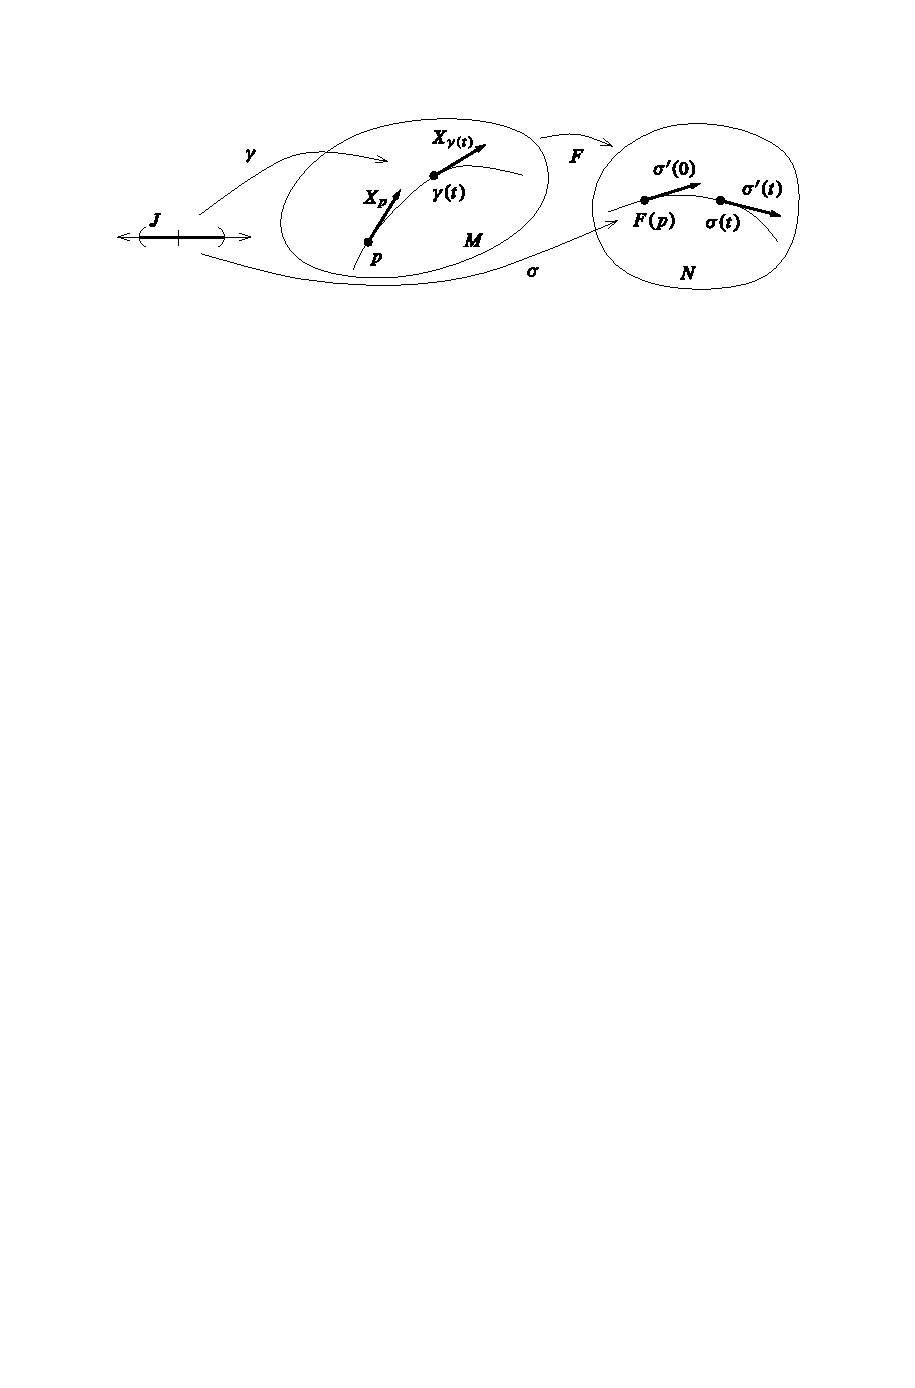
\includegraphics{pictures/integral-curve}
\caption{Flows of $F$-related vector fields.}
\end{figure}
\begin{proof}
Suppose first that $X$ and $Y$ are $F$-related, and  $\gamma:J\to M$ is an integral curve of $X$. If we define $\sigma:J\to N$ by $\sigma=F\circ\gamma$, then
\[\sigma'(t)=(F\circ\gamma)'(t)=dF_{\gamma(t)}\big(\gamma'(t)\big)=dF_{\gamma(t)}(X_{\gamma(t)})=Y_{\gamma(t)},\]
so $\sigma$ is an integral curve of $Y$.\par
Conversely, suppose $F$ takes integral curves of $X$ to integral curves of $Y$. Given $p\in M$, let $\gamma:(-\eps,\eps)\to M$ be an integral curve of $X$ starting at $p$. Since $F\circ\gamma$ is an integral curve of $Y$ starting at $F(p)$, we have
\[Y_{F(p)}=(F\circ\gamma)'(0)=dF_{p}\big(\gamma'(0)\big)=dF_p(X_p)\]
which shows that $X$ and $Y$ are $F$-related.
\end{proof}
\subsection{Flow}
Here is another way to visualize the family of integral curves associated with a vector field. Let $M$ be a smooth manifold and $V\in\X(M)$, and suppose that for each point $p\in M$, $V$ has a unique integral curve starting at $p$ and defined for all $t\in\R$, which we denote by $\theta^{(p)}:\R\to M$. (It may not always be the case that every integral curve is defined for all $t$, but for purposes of illustration let us assume so for the time being.) For each $t\in\R$, we can define a map $\theta_t:M\to M$ by sending each $p\in M$ to the point obtained by following for time $t$ the integral curve starting at $p$:
\[\theta_t(p)=\theta^{(p)}(t)\]
Each map $\theta_t$ \textit{slides} the manifold along the integral curves for time $t$. The translation lemma implies that $t\mapsto\theta^{(p)}(t+s)$ is an integral curve of $V$ starting at $q:=\theta^{(p)}(s)$; since we are assuming uniqueness of integral curves, $\theta^{(q)}(t)=\theta^{(p)}(t+s)$. When we translate this into a statement about the maps $\theta_t$, it becomes
\[\theta_t\circ\theta_s(p)=\theta_{t+s}(p)\]
Together with the equation $\theta_0(p)=p$, which holds by definition, this
implies that the map $\theta:\R\times M\to M$ is an action of the additive group $\R$ on $M$. Motivated by these observations, we define a \textbf{global flow} on $M$ (also called a \textbf{one-parameter group action}) to be a continuous left $\R$-action on $M$, that is, a continuous map $\theta:\R\times M\to M$ satisfying the following properties for all $s,t\in\R$ and $p\in M$:
\[\theta(t,\theta(s,p))=\theta(t+s,p),\quad\theta(0,p)=p.\]
Given a global flow $\theta$ on $M$, we define two collections of maps as follows:
\begin{itemize}
\item For each $t\in\R$, define a continuous map $\theta_t:M\to M$:
\[\theta_t(p)=\theta(t,p)\]
The defining properties of $\theta$ are equivalent to the \textbf{group laws}
\[\theta_t\circ\theta_s(p)=\theta_{t+s}(p),\quad\theta_0=\mathrm{id}_M.\]
As is the case for any continuous group action, each map $\theta_t:M\to M$ is a homeomorphism, and if the flow is smooth, $\theta_t$ is a diffeomorphism.
\item For each $p\in M$, define a curve $\theta^{(p)}:\R\to M$ by
\[\theta^{(p)}(t)=\theta(t,p)\]
The image of this curve is the orbit of $p$ under the group action.
\end{itemize}
The next proposition shows that every smooth global flow is derived from the
integral curves of some smooth vector field in precisely the way we described above. If $\theta:\R\times M\to M$ is a smooth global flow, for each $p\in M$ we define a tangent vector $V_p\in T_pM$ by
\[V_p=\dot{\theta}^{(p)}(0)\]
The assignment $p\mapsto V_p$ is a (rough) vector field on $M$ which is called the \textbf{infinitesimal generator of $\bm{\theta}$}, for reasons we will explain below.
\begin{proposition}\label{flow generate vector}
Let $\theta:\R\times M\to M$ be a smooth global flow on a smooth manifold $M$. The infinitesimal generator $V$ of $\theta$ is a smooth vector field on $M$, and each curve $\theta^{(p)}$ is an integral curve of $V$.
\end{proposition}
\begin{proof}
To show that $V$ is smooth, it suffices by Proposition~\ref{vector field smooth by function} to show that $Vf$ is smooth for every smooth real-valued function $f$ defined on an open subset $U\sub M$. For any such $f$ and any $p\in U$, just note that
\[Vf(p)=V_pf=\dot{\theta}^{(p)}(0)f=\frac{d}{dt}\Big|_{t=0}f\big(\theta^{(p)}(t)\big)=\frac{\partial}{\partial t}\Big|_{(0,p)}f\big(\theta(0,p)\big)\]
Because $f(\theta(t,p))$ is a smooth function of $(t,p)$ by composition, so is its partial derivative with respect to $t$. Thus, $Vf(p)$ depends smoothly on $p$, so $V$ is smooth.\par
Next we need to show that $\theta^{(p)}$ is an integral curve of $V$, which means that $\dot{\theta}^{(p)}(t)=V_{\theta^{(p)}(t)}$ for all $p\in M$ and all $t\in\R$. Let $t_0\in\R$ be arbitrary, and set $q=\theta^{(p)}(t_0)=\theta_{t_0}(p)$, so what we have to show is $\dot{\theta}^{(p)}(t_0)=V_q$. By the group law, for all $t$,
\[\theta^{(q)}(t)=\theta_t(q)=\theta_t\circ\theta_{t_0}(p)=\theta_{t+t_0}(p)=\theta^{(p)}(t+t_0)\]
Therefore, for any smooth real-valued function $f$ defined in a neighborhood of $q$,
\begin{align*}
V_qf=\dot{\theta}^{(q)}(0)f=\frac{d}{dt}\Big|_{t=0}(f\circ\theta^{(q)})(t)=\frac{d}{dt}\Big|_{t=0}(f\circ\theta^{(p)})(t+t_0)=\dot{\theta}^{(p)}(t_0)f
\end{align*}
which was to be shown.
\end{proof}
\begin{example}\label{flow eg}
The two vector fields on the plane described in Example~\ref{integral curve eg} both had integral curves defined for all $t\in\R$, so they generate global
flows. Using the results of that example, we can write down the flows explicitly.
\begin{itemize}
\item[(a)] The flow of $V=\partial/\partial x$ in $\R^2$ is the map $\tau:\R\times\R^2\to\R^2$ given by
\[\tau_t(x,y)=(x+t,y)\]
For each nonzero $t\in\R$, $\tau_t$ 0translates the plane to the right $(t>0)$ or left $(t<0)$ by a distance $|t|$.
\item[(b)] The flow of $W=x\partial/\partial y-y\partial/\partial x$ is the map $\theta:\R\times\R^2\to\R^2$ given by
\[\theta_t(x,y)=(x\cos t-y\sin t,x\sin t+y\cos t)=\begin{pmatrix}
\cos t&-\sin t\\
\sin t&\cos t
\end{pmatrix}\begin{pmatrix}
x\\
y
\end{pmatrix}\]
For each $t\in\R$, $\theta_t$ rotates the plane through an angle $t$ about the origin.
\end{itemize}
\end{example}
\subsection{The fundamental theorem on flows}
We have seen that every smooth global flow gives rise to a smooth vector field whose integral curves are precisely the curves defined by the flow. Conversely, we would like to be able to say that every smooth vector field is the infinitesimal generator of a smooth global flow. However, it is easy to see that this cannot be the case, because there are smooth vector fields whose integral curves are not defined for all $t\in\R$. Here are two examples.
\begin{example}
Let $M=\R^2-\{0\}$ with standard coordinates $(x,y)$, and let $V$ be the vector field $\partial/\partial x$ on $M$. The unique integral curve of $V$ starting at $(-1,0)\in M$ is $\gamma(t)=(t-1,0)$. However, in this case, $\gamma$ cannot be extended continuously past $t=1$. This is intuitively evident because of the hole in $M$ at the origin; to prove it rigorously, suppose $\widetilde{\gamma}$ is any continuous extension of $\gamma$ past $t=1$. Then $\gamma(t)\to\widetilde{\gamma}(1)\in\R^2-\{0\}$ as $t\to 1^-$. But we can also consider $\gamma$ as a map into $\R^2$ by composing with the inclusion $M\hookrightarrow\R^2$, and it is obvious from the formula that $\gamma(t)\to(0,0)$ as $t\mapsto 1^-$. Since limits in $\R^2$ are unique, this is a contradiction.
\end{example}
\begin{example}
For a more subtle example, let $M$ be all of $\R^2$ and let $W=x^2\partial/\partial x$. You can check easily that the unique integral curve of $W$ starting at $(1,0)$ is
\[\gamma(t)=(\frac{1}{1-t},0)\]
This curve also cannot be extended past $t=1$, because its $x$-coordinate is unbounded as $t\to 1^-$.
\end{example}
For this reason, we make the following definitions. If $M$ is a manifold, a \textbf{flow domain} for $M$ is an open subset $\mathcal{D}\sub\R\times M$ with the property that for each $p\in M$, the slice $\mathcal{D}^{(p)}=\{t\in\R:(t,p)\in\mathcal{D}\}$ is an open interval containing $0$. A \textbf{flow} on $M$ is a continuous map $\theta:\mathcal{D}\to M$ where $\mathcal{D}$ is a flow domain, that satisfies the following group laws: for all $p\in M$,
\begin{align}\label{group law-1}
\theta(0,p)=p
\end{align}
and for all $s\in\mathcal{D}^{(p)}$ and $t\in\mathcal{D}^{(\theta(s,p))}$ such that $s+t\in\mathcal{D}^{(p)}$,
\begin{align}\label{group law-2}
\theta\big(t,\theta(s,p)\big)=\theta(t+s,p)
\end{align}
\begin{figure}[htbp]
\centering
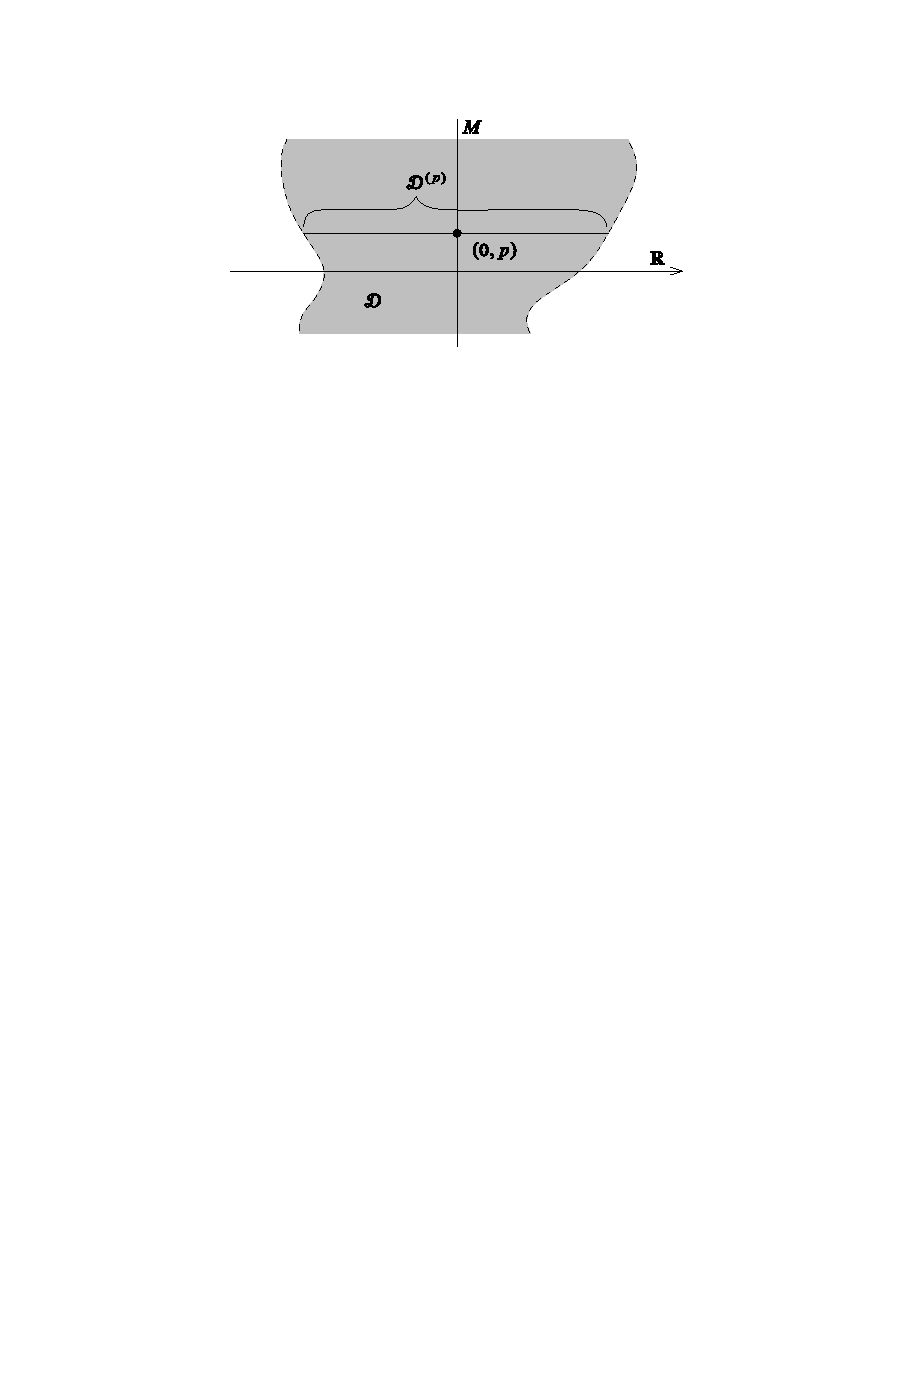
\includegraphics{pictures/flow-domain}
\caption{A flow domain.}
\end{figure}\par
We sometimes call $\theta$ a \textbf{local flow} to distinguish it from a global flow as defined earlier. The unwieldy term \textbf{local one-parameter group action} is also used.\par
If $\theta$ is a flow, we define $\theta_t(p)=\theta(t,p)$ whenever $(t,p)\in\mathcal{D}$, just as for a global flow. For each $t\in\R$, we also define
\[M_t=\{p\in M:(t,p)\in\mathcal{D}\}\]
so that
\[p\in M_t\iff t\in\mathcal{D}^{(p)}\iff(t,p)\in\mathcal{D}\]
If $\theta$ is smooth, the infinitesimal generator of $\theta$ is defined by $V_p=\dot{\theta}^{(p)}(0)$.
\begin{proposition}
If $\theta:\mathcal{D}\to M$ is a smooth flow, then the infinitesimal generator $V$ of $\theta$ is a smooth vector field, and each curve $\theta^{(p)}$ is an integral curve of $V$.
\end{proposition}
\begin{proof}
The proof is essentially identical to the analogous proof for global flows, Proposition~\ref{flow generate vector}. In the proof that $V$ is smooth, we need only note that for any $p_0\in M$, $\theta(t,p)$ is defined and smooth for all $(t,p)$ sufficiently close to $(0,p_0)$ because $\mathcal{D}$ is open. In the proof that $\theta^{(p)}$ is an integral curve, we need to verify that all of the expressions make sense. Suppose $t_0\in\mathcal{D}^{(p)}$. Because both $\mathcal{D}^{(p)}$ and $\mathcal{D}^{(\theta_{t_0}(p))}$ are open intervals containing $0$, there is a positive number $\eps$ such that $t+t_0\in\mathcal{D}^{(p)}$ and $t\in\mathcal{D}^{(\theta_{t_0}(p))}$ whenever $|t|<\eps$, and then $\theta_t(\theta_{t_0}(p))=\theta_{t+t_0}(p)$ by definition of a flow. The rest of the proof goes through just as before.
\end{proof}
The next theorem is the main result of flows. A \textbf{maximal integral curve} is one that cannot be extended to an integral curve on any larger open interval, and a \textbf{maximal flow} is a flow that admits no extension to a flow on a larger flow domain.
\begin{theorem}[\textbf{Fundamental Theorem on Flows}]\label{flow fundamental thm}
Let $V$ be a smooth vector field on a smooth manifold $M$. There is a unique smooth maximal flow $\theta:\mathcal{D}\to M$ whose infinitesimal generator is $V$. This flow has the following properties:
\begin{itemize}
\item[(a)] For each $p\in M$, the curve $\theta^{(p)}:\mathcal{D}^{(p)}\to M$ is the unique maximal integral curve of $V$ starting at $p$.
\item[(b)] If $s\in\mathcal{D}^{(p)}$, then $\mathcal{D}^{(\theta(s,p))}$ is the interval $\mathcal{D}^{(p)}-s=\{t-s:t\in\mathcal{D}^{(p)}\}$.
\item[(c)] For each $t\in\R$, the set $M_t$ is open in $M$, and $\theta_t:M_t\to M_{-t}$ is a diffeomorphism with inverse $\theta_{-t}$.
\end{itemize}
\end{theorem}
\begin{proof}
Proposition~\ref{integral curve local exsit} shows that there exists an integral curve starting at each point $p\in M$. Suppose $\gamma,\widetilde{\gamma}:J\to M$ are 
two integral curves of $V$ defined on the same open interval $J$ such that $\gamma(t_0)=\widetilde{\gamma}(t_0)$ for some $t_0\in J$. Let $\mathcal{S}$ be the set 
of $t\in J$ such that $\gamma(t)=\widetilde{\gamma}(t)$. Clearly, $\mathcal{S}\neq\emp$, because $t_0\in\mathcal{S}$ by hypothesis, and $\mathcal{S}$ is closed in 
$J$ by continuity. On the other hand, suppose $t_1\in\mathcal{S}$. Then in a smooth coordinate neighborhood around the point $p=\gamma(t_1)$, $\gamma$ and 
$\widetilde{\gamma}$ are both solutions to same ODE with the same initial condition $\gamma(t_1)=\widetilde{\gamma}(t_1)=p$. By the uniqueness theorem of ODEs, 
$\gamma\equiv\widetilde{\gamma}$ on an interval containing $t_1$, which implies that $\mathcal{S}$ is open in $J$. Since $J$ is connected, $\mathcal{S}=J$, which 
implies that $\gamma\equiv\widetilde{\gamma}$ on all of $J$. Thus, any two integral curves that agree at one point agree on their common domain.\par
For each $p\in M$, let $\mathcal{D}^{(p)}$ be the union of all open intervals $J\sub\R$ containing $0$ on which an integral curve starting at $p$ is defined. 
Define $\theta^{(p)}:\mathcal{D}^{(p)}\to M$ by letting $\theta^{(p)}(t)=\gamma(t)$, where $\gamma$ is any integral curve starting at $p$ and defined on an open 
interval containing $0$ and $t$. Since all such integral curves agree at $t$ by the argument above, $\theta^{(p)}(t)$ is well defined, and is obviously the unique 
maximal integral curve starting at $p$.\par
Now let $\mathcal{D}=\{(t,p)\in\R\times M:t\in\mathcal{D}^{(p)}\}$ and define $\theta(t,p)=\theta^{(p)}(t)$. As usual, we also write $\theta_t(p)=\theta(t,p)$. 
By definition, $\theta$ satisfies property (a) in the statement of the fundamental theorem: for each $p\in M$, $\theta^{(p)}(t)$ is the unique maximal integral 
curve of $V$ starting at $p$. To verify the group laws, fix any $p\in M$ and $s\in\mathcal{D}^{(p)}$, and write $q=\theta(s,p)=\theta^{(p)}(s)$. The curve 
$\gamma:\mathcal{D}^{(p)}-s\to M$ defined by $\gamma(t)=\theta^{(p)}(t+s)$ starts at $q$, and the translation lemma shows that $\gamma$ is an integral curve 
of $V$. By uniqueness of ODE solutions, $\gamma$ agrees with $\theta^{(q)}$ on their common domain, which is equivalent to the second group law $(\ref{group law-2})$, 
and the first group law $(\ref{group law-1})$ is immediate from the definition. By maximality of $\theta^{(q)}$, the domain of $\gamma$ cannot be larger than 
$\mathcal{D}^{(q)}$, which means that $\mathcal{D}^{(p)}-s\sub\mathcal{D}^{(q)}$. Since $0\in\mathcal{D}^{(p)}$, this implies that $-s\in\mathcal{D}^{(q)}$, and 
the group law implies that $\theta^{(q)}(-s)=p$. Applying the same argument with $(-s,q)$ in place of $(s,p)$, we find that $\mathcal{D}^{(q)}+s\sub\mathcal{D}^{(p)}$, 
which is the same as $\mathcal{D}^{(q)}\sub\mathcal{D}^{(p)}-s$. This proves (b).\par
Next we show that $\mathcal{D}$ is open in $\R\times M$ (so it is a flow domain), and that $\theta:\mathcal{D}\to M$ is smooth. Define a subset $W\sub\mathcal{D}$ 
as the set of all $(t,p)\in\mathcal{D}$ such that $\theta$ is defined and smooth on a product neighborhood of $(t,p)$ of the form $J\times U$ where $J\sub\R$ is 
an open interval containing $0$ and $t$, $U\sub M$ is a neighborhood of $p$. Then $W$ is open in $\R\times M$, and the restriction of $\theta$ to $W$ is smooth, 
so it suffices to show that $W=\mathcal{D}$. Suppose this is not the case. Then there exists some point $(\tau,p_0)\in\mathcal{D}-W$. For simplicity, assume $\tau>0$, 
the argument for $\tau<0$ is similar.
\begin{figure}[htbp]
\centering
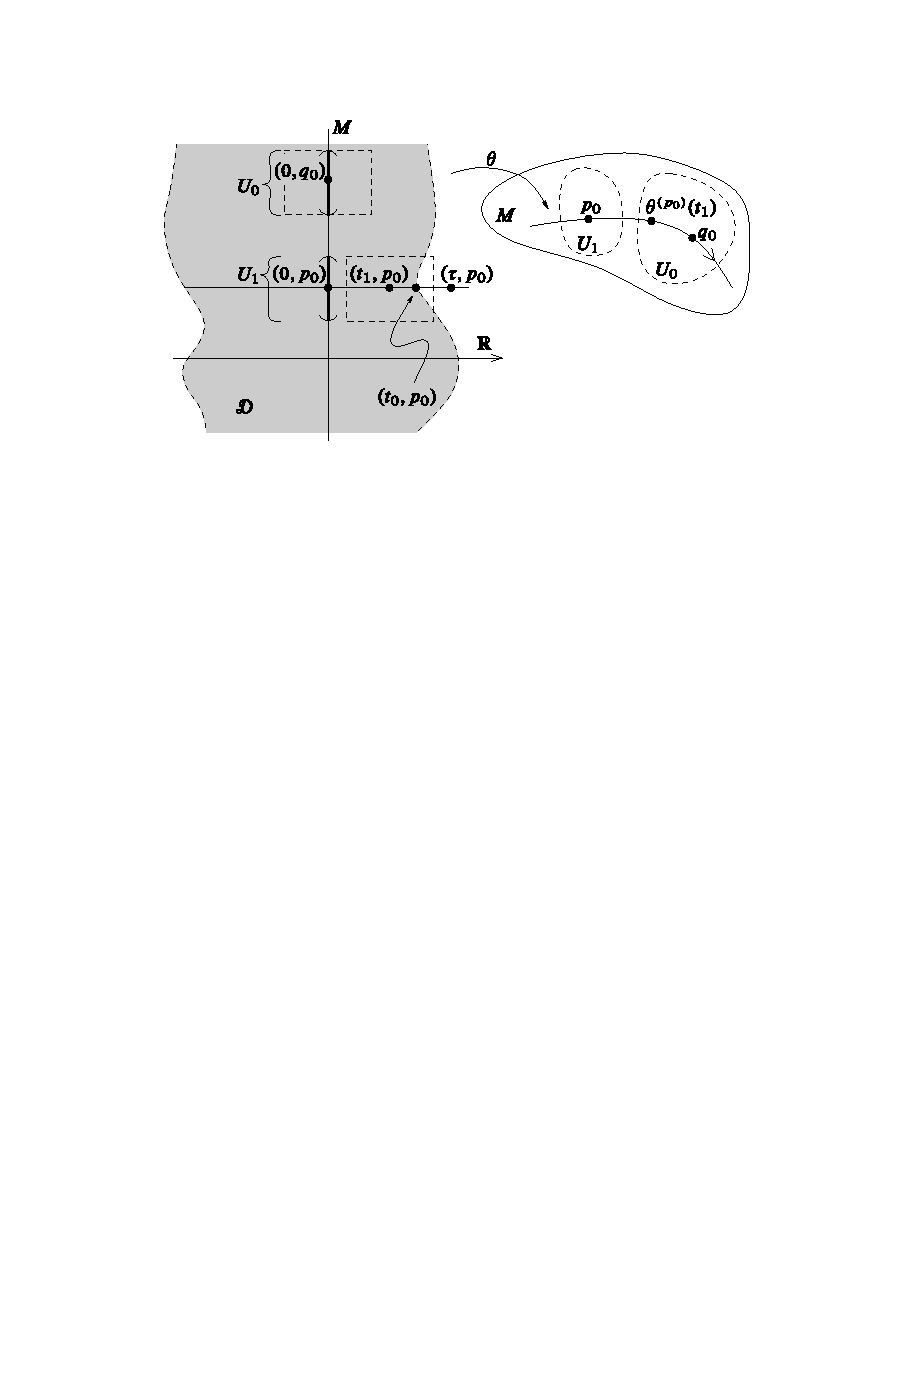
\includegraphics{pictures/flow-thm}
\caption{Proof that $\mathcal{D}$ is open.}
\end{figure}\par
Let $t_0=\sup\{t\in\R:(t,p_0)\in W\}$. By the existence and uniquess theorem of ODEs applied in
smooth coordinates around $p_0$, we know that $\theta$ is defined and smooth in some product neighborhood of $(0,p_0)$, so $t_0>0$. Since $t_0\leq\tau$ and $\mathcal{D}^{(p_0)}$ is an open interval containing $0$ and $\tau$, it follows that $t_0\in\mathcal{D}^{(p_0)}$. Let $q_0=\theta^{(p_0)}(t_0)$. By the ODE theorem again, there exist $\eps>0$ and a neighborhood $U_0$ of $q_0$ such that $(-\eps,\eps)\times U_0\sub W$. We will use the group law to show that $\theta$ extends smoothly to a neighborhood of $(t_0,p_0)$, which is a contradiction.\par
Choose some $t_1<t_0$ such that $t_1+\eps>t_0$ and $\theta^{(p_0)}(t_1)\in U_0$. Since $t_1<t_0$, we have $(t_1,p_0)\in W$, and so there is a product neighborhood $(t_1-\delta,t_1+\delta)\times U_1\sub W$. Because $\theta(t_1,p_0)\in U_0$, we can choose $U_1$ small enough that $\theta$ maps $\{t_1\}\times U_1$ into $U_0$. Define $\widetilde{\theta}:[0,t_1+\eps)\times U_1\to M$ by
\[\widetilde{\theta}(t,p)=\begin{cases}
\theta_t(p)&p\in U_1,0\leq t\leq t_1,\\
\theta_{t-t_1}\circ\theta_{t_1}(p)&p\in U_1,t_1-\eps<t<t_1+\eps
\end{cases}\]
The group law for $\theta$ guarantees that these definitions agree where they overlap, and our choices of $U_1,t_1$, and $\theta$ ensure that this defines a smooth map. By the translation lemma, each map $t\mapsto\theta_t(p)$ is an integral curve of $V$, so $\widetilde{\theta}$ is a smooth extension of $\theta$ to a neighborhood of $(t_0,p_0)$, contradicting our choice of $t_0$. This completes the proof that $W=\mathcal{D}$.\par
Finally, we prove (c). The fact that $M_t$ is open is an immediate consequence of the fact that $\mathcal{D}$ is open. From part (b) we deduce
\begin{align*}
p\in M_t\Rightarrow t\in\mathcal{D}^{(p)}\Rightarrow\mathcal{D}^{(\theta_t(p))}=\mathcal{D}^{(p)}-t\Rightarrow-t\in\mathcal{D}^{(\theta_t(p))}\Rightarrow\theta_t(p)\in M_{-t}
\end{align*}
which shows that $\theta_t$ maps $M_t$ to $M_{-t}$. Moreover, the group laws then show that $\theta_{-t}\circ\theta_{t}$ is equal to the identity on $M_t$. Reversing the roles of $t$ and $-t$ shows that $\theta_{t}\circ\theta_{-t}$ is the identity on $M_{-t}$, which completes the proof.
\end{proof}
The flow whose existence and uniqueness are asserted in the fundamental theorem is called the \textbf{flow generated by $\bm{V}$}, or just the \textbf{flow of $\bm{V}$}. Now we give an example of this.
\begin{figure}[htbp]
\centering
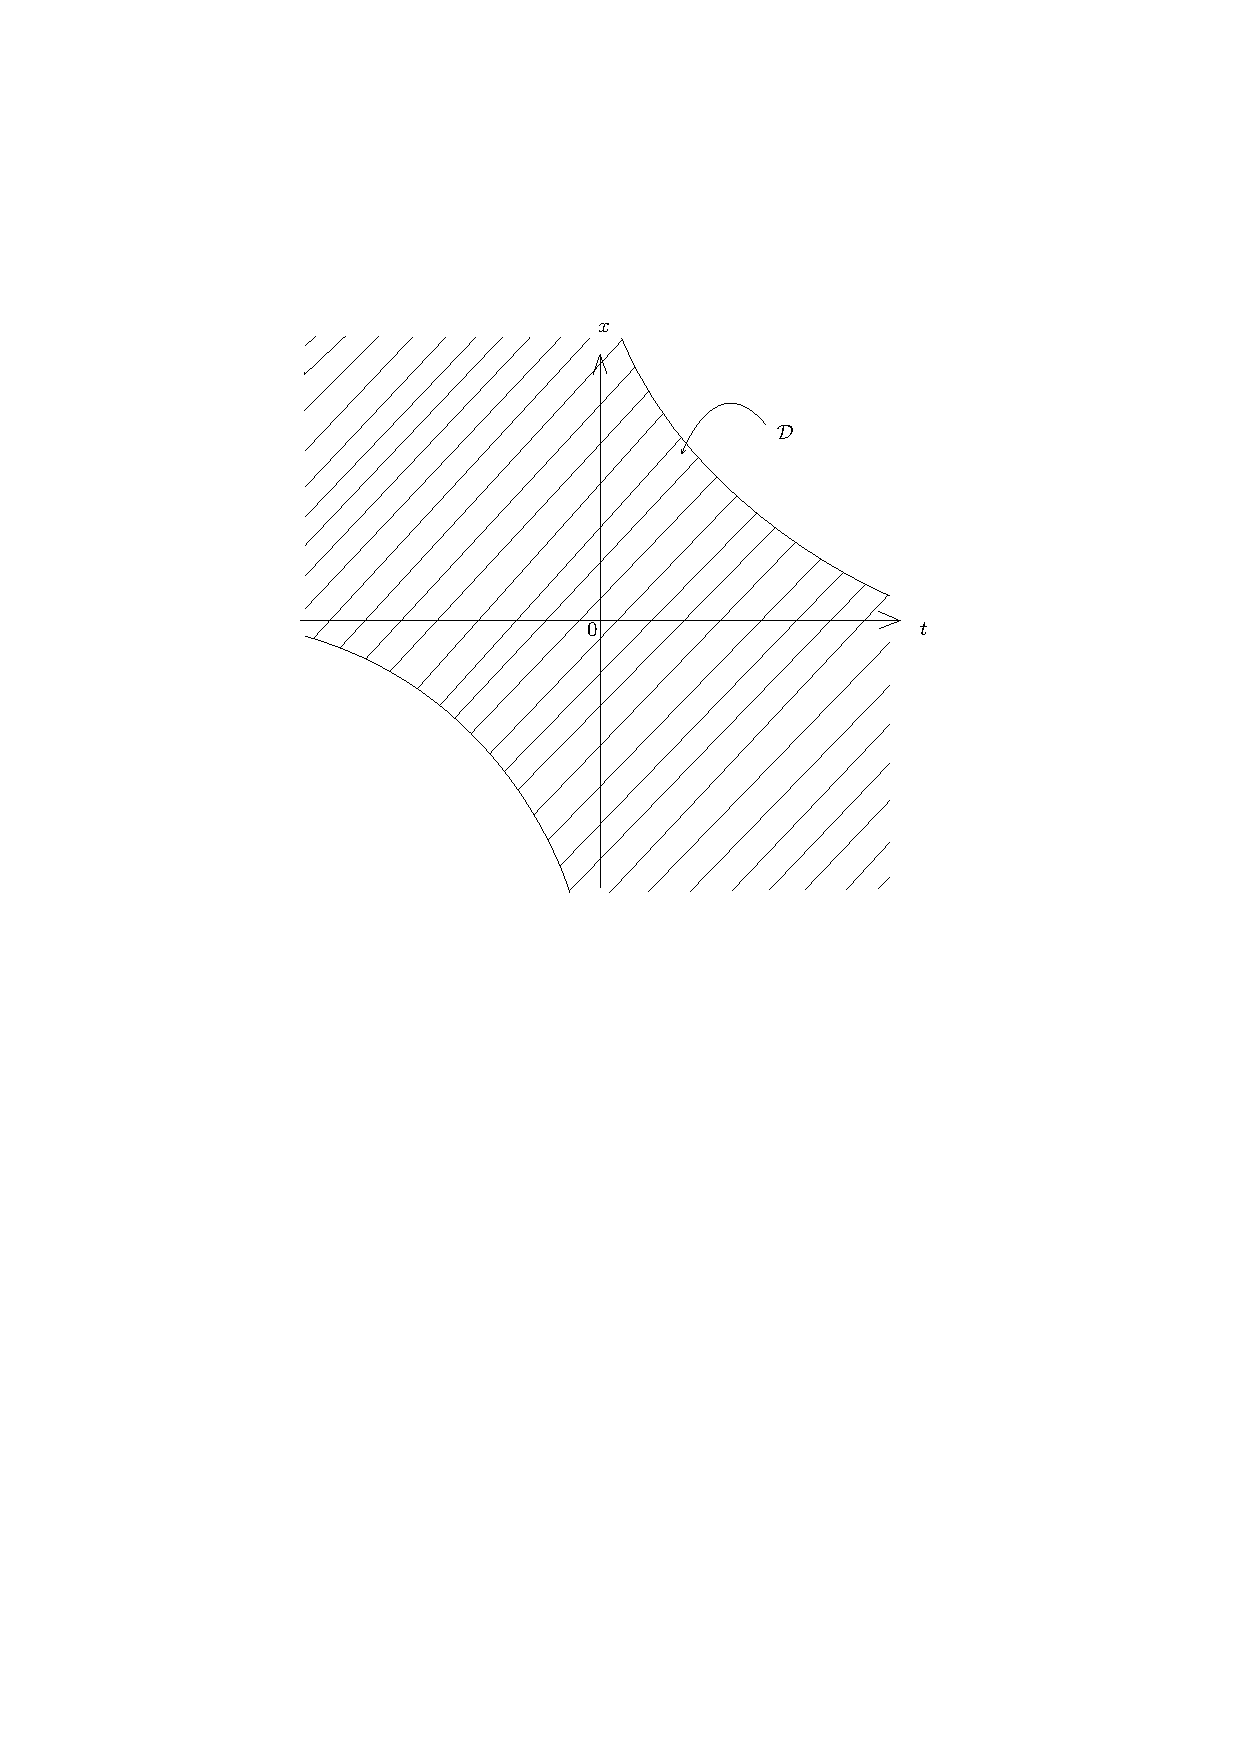
\includegraphics[width=0.5\textwidth]{pictures/flow-domain-eg}
\caption{The flow domain in Example~\ref{flow doamin eg}.}
\end{figure}
\begin{example}\label{flow doamin eg}
Let $V=x^2\partial/\partial x$ be a vector field on $\R$, we can check that the unique integral curve of $V$ starting at $x$ is
\[\theta(t,x)=\gamma_x(t)=\begin{cases}
\dfrac{1}{x^{-1}-t}&x\neq 0;\\
0&x=0.
\end{cases}\]
Thus the flow domain of $V$ is 
\[\mathcal{D}=\{(t,x):t>0,x<1/t\}\cup\{(t,x):t<0,x>1/t\}.\]

Now for $x>0$ and $t\in(-\infty,1/x)$, we check that
\[\theta(t,x)=\frac{1}{x^{-1}-t},\quad \mathcal{D}^{(\theta(t,x))}=(-\infty,\frac{1}{x}-t)=\mathcal{D}^{(x)}-t.\]
\end{example}
\begin{theorem}[\textbf{Naturality of Flows}]\label{flow naturality}
Suppose $M$ and $N$ are smooth manifolds, $F:M\to N$ is a smooth map, $X\in\X(M)$, and $Y\in\X(N)$. Let $\theta$ be the flow of $X$ and $\eta$ the flow of $Y$. If $X$ and $Y$ are $F$-related, then for each $t\in\R$, $F(M_t)\sub N_t$ and $\eta_t\circ F=F\circ\theta_t$ on $M_t$:
\[\begin{tikzcd}
M_t\ar[d,"\theta_t"]\ar[r,"F"]&N_t\ar[d,"\eta_t"]\\
M_{-t}\ar[r,"F"]&N_{-t}
\end{tikzcd}\]
\end{theorem}
\begin{proof}
By Proposition~\ref{integral curve naturality}, for any $p\in M$, the curve $F\circ\theta^{(p)}$ is an integral curve of $Y$ starting at $F\circ\theta^{(p)}(0)=F(p)$. By uniqueness of integral curves, therefore, the maximal integral curve $\eta^{(F(p))}$ must be defined at least on the interval $\mathcal{D}^{(p)}$, and $F\circ\theta^{(p)}=\eta^{(F(p))}$ on that interval. This means that
\[p\in M_t\Rightarrow t\in\mathcal{D}^{(p)}\Rightarrow t\in\mathcal{D}^{(F(p))}\Rightarrow F(p)\in N_t,\]
which is equivalent to $F(M_t)\sub N_t$, and
\[F\big(\theta^{(p)}(t)\big)=\eta^{(F(p))}(t)\for t\in\mathcal{D}^{(p)}\]
which is equivalent $\eta_t\circ F=F\circ\theta_t$ for all $p\in M_t$.
\end{proof}
The next corollary is immediate.
\begin{corollary}[\textbf{Diffeomorphism Invariance of Flows}]
Let $F:M\to N$ be a diffeomorphism. If $X\in\X(M)$ and $\theta$ is the flow of $X$, then the flow of $F^*X$ is $\eta_t=F\circ\theta_t\circ F^{-1}$, with domain $N_t=F(M_t)$ for each $t\in\R$.
\end{corollary}
\subsubsection{Complete vector fields}
As we observed earlier in this chapter, not every smooth vector field generates a global flow. The ones that do are important enough to deserve a name. We say that a smooth vector field is \textbf{complete} if it generates a global flow, or equivalently if each of its maximal integral curves is defined for all $t\in\R$.\par
We will show below that all compactly supported smooth vector fields, and therefore all smooth vector fields on a compact manifold, are complete. The proof will be based on the following lemma.
\begin{lemma}[\textbf{Uniform Time Lemma}]
Let $V$ be a smooth vector field on a smooth manifold $M$, and let $\theta$ be its flow. Suppose there is a positive number $\eps$ such that for every $p\in M$, the domain of $\theta^{(p)}$ contains $(-\eps,\eps)$. Then $V$ is complete.
\end{lemma}
\begin{proof}
Suppose for the sake of contradiction that for some $p\in M$, the domain $\mathcal{D}^{(p)}$ of $\theta^{(p)}$ is bounded above. (A similar proof works if it is bounded below.) Let $b=\sup\mathcal{D}^{(p)}$, let $t_0$ be a positive number such that $b-\eps<t_1<b$, and let $q=\theta^{(p)}(t_0)$. The hypothesis implies that $\theta^{(q)}(t)$ is defined at least for $t\in(-\eps,\eps)$. Define a curve $\gamma:(-\eps,t_0+\eps)\to M$ by
\[\gamma(t)=\begin{cases}
\theta^{(p)}(t),&-\eps<t<b\\
\theta^{(q)}(t-t_0),&t_0-\eps<t<t_0+\eps
\end{cases}\]
These two definitions agree where they overlap, because
\[\theta^{(q)}(t-t_0)=\theta_{t-t_0}(q)=\theta_{t-t_0}\theta_{t_0}(p)=\theta_t(p)\]
by the group law for $\theta$. By the translation lemma, $\gamma$ is an integral curve starting at $p$. Since $t_0+\eps>b$, this is a contradiction.
\end{proof}
\begin{theorem}\label{vector field compact supp complete}
Every compactly supported smooth vector field on a smooth manifold is complete.
\end{theorem}
\begin{proof}
Suppose $V$ is a compactly supported vector field on a smooth manifold $M$, and let $K=\supp(V)$. For each $p\in K$, there is a neighborhood $U_p$ of $p$ and a positive number $\eps_p$ such that the flow of $V$ is defined at least on $(-\eps_p,\eps_p)\times U_p$. By compactness, finitely many such sets $U_{p_1},\dots,U_{p_k}$ cover $K$. With $\eps:=\min\{\eps_{p_i}\}$, it follows that every maximal integral curve starting in $K$ is defined at least on $(-\eps,\eps)$. Since $V\equiv 0$ outside of $K$, every integral curve starting in $M-K$ is constant and thus can be defined on all of $\R$. Thus the hypotheses of the uniform time lemma are satisfied, so $V$ is complete.
\end{proof}
\begin{corollary}\label{vector field compact mani complete}
On a compact smooth manifold, every smooth vector field is
complete.
\end{corollary}
Left-invariant vector fields on Lie groups form another class of vector fields that are always complete.
\begin{theorem}\label{vector field left-inva complete}
Every left-invariant vector field on a Lie group is complete.
\end{theorem}
\begin{proof}
Let $G$ be a Lie group, let $X\in\Lie(G)$, and let $\theta:\mathcal{D}\to G$ denote the flow of $X$. There is some $\eps>0$ such that $\theta^{(e)}$ is defined on $(-\eps,\eps)$.\par Let $g\in G$ be arbitrary. Because $X$ is $L_g$-related to itself, it follows from Proposition~\ref{integral curve naturality} that the curve $L_g\circ\theta^{(e)}$ is an integral curve of $X$ starting at $g$ and therefore is equal to $\theta^{(g)}$. This shows that for each $g\in G$, the integral curve $\theta^{(p)}$ is defined at least on $(-\eps,\eps)$, so the uniform time lemma guarantees that $X$ is complete.
\end{proof}
Here is another useful property of integral curves.
\begin{lemma}[\textbf{Escape Lemma}]\label{vector flow escape lemma}
Suppose $M$ is a smooth manifold and $V\in\X(M)$. If $\gamma:J\to M$ is a maximal integral curve of $V$ whose domain $J$ has a finite least upper bound $b$, then for any $t_0\in J$, the set $\gamma\big([t_0,b)\big)$ is not contained in any compact subset
of $M$.
\end{lemma}
\begin{proof}
Let $p=\gamma(0)$ and $\theta$ denote the flows of $V$ so that $\gamma(t)=\theta^{(p)}(t)$. Assume 
that there is a $t_0\in J$ such that $\gamma\big([t_0,b)\big)$ lies in a compact set $K\sub M$, we 
claim that $\gamma$ can be extended past $b$.
\begin{itemize}
\item We use sequentially compactness: let $(x_n)$ be any sequence tends to $b$ from below, since $\{\gamma(x_n)\}$ is contained in a compact set, it has a subsequence converging to a point $q\in M$.
\item By theorem~\ref{flow fundamental thm}, there is $\eps>0$ and a neighborhood of $q$ such that $\theta$ is defined on $(-\eps,\eps)\times U$.
\item By discrading finitely many terms, we may assume that $\gamma(x_i)\in U$ and $t_i>b-\eps$. Then define $\sigma:[t_0,b+\eps)\to M$ by
\[\sigma(t)=\begin{cases}
\gamma(t)&t_0\leq t<b,\\
\theta_{t-t_i}\circ\theta_{t_i}(p),&t_i-\eps<t<t_i+\eps.
\end{cases}\]
This map is defined for all $t\in[b,b+\eps)$ since $t_i\to b$, and the two definitions agree where they overlap, as
\[\theta_{t-t_i}\circ\theta_{t_i}(p)=\theta_t(p)=\gamma(t)\]
\end{itemize}
This contradicts the maximality, so our claim follows.
\end{proof}
\subsection{Flowouts}
Flows provide the technical apparatus for many geometric constructions on manifolds. Most of those constructions are based on the following general theorem,
which describes how flows behave in the vicinity of certain submanifolds.
\begin{theorem}[\textbf{Flowout Theorem}]\label{flowout}
Suppose $M$ is a smooth manifold, $S\sub M$ is an embedded $k$-dimensional submanifold, and $V\sub\X(M)$ is a smooth vector field that is nowhere tangent to $S$. Let $\theta:\mathcal{D}\to M$ be the flow of $V$, let $\mathcal{O}=(\R\times S)\cap\mathcal{D}$, and let $\varPhi=\theta|_{\mathcal{O}}$.
\begin{itemize}
\item[(a)] $\varPhi:\mathcal{O}\to M$ is an immersion.
\item[(b)] $\partial/\partial t\in\X(\mathcal{O})$ is $\varPhi$-related to $V$.
\item[(c)] There exists a smooth positive function $\delta:S\to\R$ such that the restriction of $\varPhi$ to $\mathcal{O}_{\delta}$ is injective, where $\mathcal{O}_{\delta}\sub\mathcal{O}$ is the flow domain
\begin{align}\label{flowout thm-1}
\mathcal{O}_{\delta}=\{(t,p)\in\mathcal{O}:|t|<\delta(p)\}
\end{align}
Thus, $\varPhi(\mathcal{O}_{\delta})$ is an immersed submanifold of $M$ containing $S$, and $V$ is tangent to this submanifold.
\item[$(d)$] If $S$ has codimension $1$, then $\varPhi|_{\mathcal{O}_\delta}$ is a diffeomorphism onto an open submanifold of $M$.
\end{itemize}
\end{theorem}
\begin{figure}[htbp]
\centering
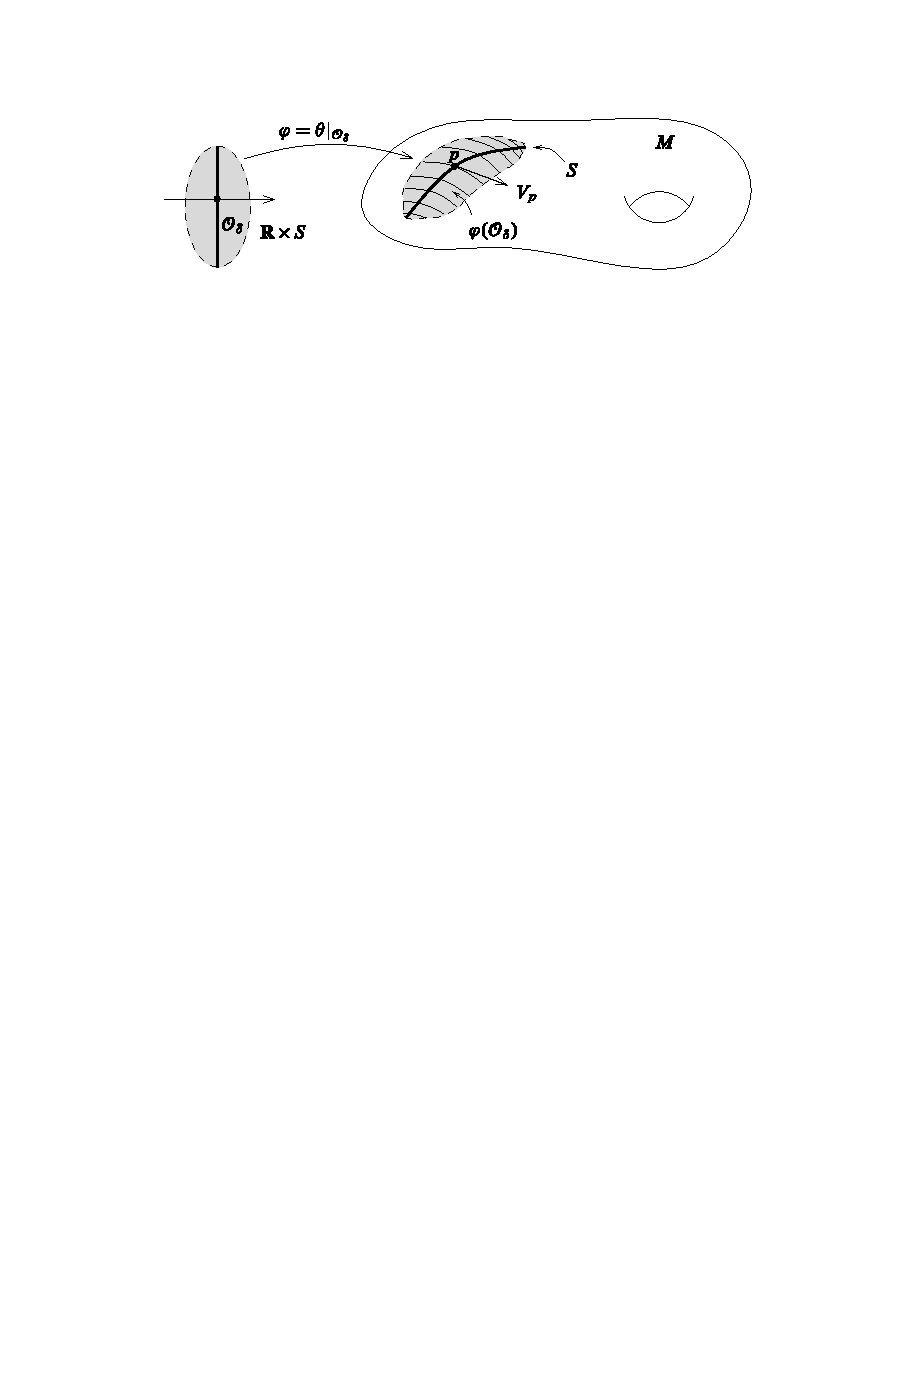
\includegraphics{pictures/flowout}
\caption{A flowout.}
\end{figure}
\begin{remark}
The submanifold $\varPhi({\mathcal{O}_\delta})\sub M$ is called a \textbf{flowout from $S$ along $V$}.
\end{remark}
\begin{proof}
First we prove (b). Fix some $p\in S$, and let $\sigma:\mathcal{D}^{(p)}\to\R\times S$ be the curve $\sigma(t)=(t,p)$. Then $\varPhi\circ\sigma(t)=\theta(t,p)$ is an integral curve of $V$, so for any $t_0\in\mathcal{D}^{(p)}$ it follows that
\[d\varPhi_{(t_0,p)}\Big(\frac{\partial}{\partial t}\Big|_{(t_0,p)}\Big)=(\varPhi\circ\sigma)'(t_0)=V_{\varPhi(t_0,p)}.\]

Next we prove (a). The restriction of $\varPhi$ to $\{0\}\times S$ is the composition of the diffeomorphism $\{0\}\times S\approx S$ with the embedding $S\hookrightarrow M$, so it is an embedding. Thus, the restriction of $d\varPhi_{(0,p)}$ to $T_pS$ (viewed as a subspace of $T_{(0,p)}\mathcal{O}\cong T_0\R\oplus T_pS$) is the inclusion $T_pS\hookrightarrow T_pM$. If $(E_1,\dots,E_k)$ is any basis for $T_pS$, it follows that $d\varPhi_{(0,p)}$ maps the basis $(\partial/\partial t|_{(0,p)},E_1,\dots,E_k)$ for $T_{(0,p)}\mathcal{O}$ to $(V_p,E_1,\dots,E_k)$. Since $V_p$ is not tangent to $S$, this $(k+1)$-tuple is linearly independent and thus $d\varPhi_{(0,p)}$ is injective.\par
To show $d\varPhi$ is injective at other points, we argue as in the proof of the equivariant rank theorem. Given $(t_0,p_0)\in\mathcal{O}$, let $\tau_{t_0}:\mathcal{O}\to\R\times S$ be the translation $\tau_{t_0}(t,p)=(t+t_0,p)$. By the group law for $\theta$, the following diagram commutes (where the horizontal maps might be defined only in open subsets containing $(0,p_0)$ and $p_0$, respectively):
\[\begin{tikzcd}
\mathcal{O}\ar[r,"\tau_{t_0}"]\ar[d,swap,"\varPhi"]&\mathcal{O}\ar[d,"\varPhi"]\\
M\ar[r,"\theta_{t_0}"]&M
\end{tikzcd}\]
Both horizontal maps in the diagram above are local diffeomorphisms. Taking differentials, we obtain
\[\begin{tikzcd}
T_{(0,p_0)}\mathcal{O}\ar[rr,"d(\tau_{t_0})_{(0,p_0)}"]\ar[d,swap,"d\varPhi_{(0,p_0)}"]&&T_{(t_0,p_0)}\mathcal{O}\ar[d,"d\varPhi_{(t_0,p_0)}"]\\
T_{p_0}M\ar[rr,"d(\theta_{t_0})_{p_0}"]&&T_{\varPhi(t_0,p_0)}M
\end{tikzcd}\]
Because the horizontal maps are isomorphisms, the two vertical maps have the same
rank. Since we have already shown that $d\varPhi_{(0,p_0)}$ has full rank, so does $d\varPhi_{(t_0,p_0)}$. This completes the proof that $\varPhi$ is an immersion.\par
Next we prove (c). Given a point $p_0\in S$, choose a slice chart $(U,(x^i))$ for $S$ in $M$ centered at $p_0$, so that $U\cap S$ is the set where $x^{k+1}=\cdots=x^n=0$ (where $n=\dim M$). Because $V$ is not tangent to $S$, one of the last $n-k$ components of $V_{p_0}$, say $V^j_{p_0}$, must be nonzero. Shrinking $U$ if necessary, we may assume that there is a constant $c>0$ such that
\begin{align}\label{flowout thm-2}
|V^j_p|\geq c\for p\in U.
\end{align}
Since $\varPhi^{-1}(U)$ is open in $\R\times S$, we may choose a number $\eps_{p_0}>0$ and a neighborhood $W_{p_0}$ of $p_0$ in $S$ such that $(-\eps_{p_0},\eps_{p_0})\times W_{p_0}\sub\mathcal{O}$ and $\varPhi\big((-\eps_{p_0},\eps_{p_0})\times W_{p_0}\big)\sub U$. Write the component functions of $\varPhi$ in these local coordinates as
\[\varPhi(t,p)=\big(\varPhi^1(t,p),\dots,\varPhi^n(t,p)\big)\]
Because $\varPhi$ is the restriction of the flow, the component function $\varPhi^j$ satisfies
\[\frac{\partial\varPhi^j}{\partial t}(t,p)=V^j\big(\varPhi(t,p)\big),\quad\varPhi^j(0,p)=p\]
By $(\ref{flowout thm-2})$ and the fundamental theorem of calculus, $|\varPhi^j(t,p)|\geq c|t|$, and thus for $(t,p)\in(-\eps_{p_0},\eps_{p_0})\times W_{p_0}$ we conclude that $\varPhi(t,p)\in S$ if and only if $t=0$.\par
Choose a smooth partition of unity $\{\psi_p:p\in S\}$ subordinate to the open cover $\{W_p:p\in S\}$ of $S$, and define $f:S\to\R$ by
\[f(q)=\sum_{p\in S}\eps_p\psi_p(q)\]
Then $f$ is smooth and positive. For each $q\in S$, there are finitely many $p\in S$ such that $\psi_p(q)>0$; if $p_1$ is one of these points such that $\eps_{p_1}$ is maximum among all such $\eps_p$, then
\[f(q)\leq\eps_{p_1}\sum_{p\in S}\psi_p(q)=\eps_{p_1}\]
It follows that if $(t,q)\in\mathcal{O}$ such that $|t|<f(q)$, then $(t,q)\in(-\eps_{p_1},\eps_{p_1})\times W_{p_1}$, so $\varPhi(t,q)\in S$ if and only if $t=0$.\par
Let $\delta=f/2$. We will show that $\varPhi|_{\mathcal{O}_\delta}$ is injective, where $\mathcal{O}_{\delta}$ is defined by $(\ref{flowout thm-1})$. Suppose $\varPhi(t,q)=\varPhi(t',q')$ for some $(t,q),(t',q')\in\mathcal{O}_{\delta}$. By renaming the points if necessary, we may arrange that $f(q')\leq f(q)$. Our assumption means that $\theta_t(q)=\theta_{t'}(q')$, and the group law for $\theta$ then implies that $\theta_{t-t'}(q)=q'\in S$. The fact that $(t,q)$ and $(t',q')$ are in $\mathcal{O}_\delta$ implies that
\[|t-t'|\leq|t|+|t'|\leq\frac{1}{2}f(q)+\frac{1}{2}f(q')\leq f(q)\]
which forces $|t-t'|=0$ by our previous argument, and thus $q=q'$.\par
Only $(d)$ remains. If $S$ has codimension $1$, then $\varPhi|_{\mathcal{O}_\delta}$ is an injective smooth immersion between manifolds of the same dimension, so it is an embedding (Proposition~\ref{smooth embedd if}$(d)$) and a diffeomorphism onto an open submanifold (Proposition~\ref{open submani iff}).
\end{proof}
\subsubsection{Regular points and singular points}
If $V$ is a vector field on $M$, a point $p\in M$ is said to be a singular point of $V$ if $V_p=0$, and a regular point otherwise. The next proposition shows that the integral curves starting at regular and singular points behave very differently from each other.
\begin{proposition}\label{flow regular singular}
Let $V$ be a smooth vector field on a smooth manifold $M$, and let $\theta:\mathcal{D}\to M$ be the flow generated by $V$. If $p\in M$ is a singular point of $V$, then $\mathcal{D}^{(p)}=\R$ and $\theta^{(p)}$ is the constant curve $\theta^{(p)}(t)=p$. If $p$ is a regular point, then $\theta^{(p)}:\mathcal{D}^{(p)}\to M$ is a smooth immersion.
\end{proposition}
\begin{proof}
If $V_p=0$, then the constant curve $\gamma:\R\to M$ given by $\gamma(t)=p$ is clearly an integral curve of $V$, so by uniqueness and maximality it must be equal to $\theta^{(p)}$.\par
To verify the second statement, we prove its contrapositive: if $\theta^{(p)}$ is not an immersion, then $p$ is a singular point. The assumption that $\theta^{(p)}$ is not an immersion
means that $\det{\theta}^{(p)}(s)=0$ for some $s\in\mathcal{D}^{(p)}$. Write $q=\theta^{(p)}(s)$. Then the argument in the preceding paragraph implies that $\mathcal{D}^{(q)}=\R$ and $\theta^{(q)}(t)=q$ for all $t\in\R$. It follows from Theorem~\ref{flow fundamental thm}(b) that $\mathcal{D}^{(p)}=\R$ as well, and for all $t\in\R$ the group law gives
\[\theta^{(p)}(t)=\theta_t(p)=\theta_{t-s}\circ\theta_s(p)=\theta_{t-s}(q)=q.\]
Setting $t=0$ yields $p=q$, and thus $\theta^{(p)}(t)\equiv p$ and $V_p=0$.
\end{proof}
If $\theta:\mathcal{D}\to M$ is a flow, a point $p\in M$ is called an \textbf{equilibrium point} of $\theta$ if $\theta(t,p)=p$ for all $t\in\mathcal{D}^{(p)}$. Proposition~\ref{flow regular singular} shows that the equilibrium points of a smooth flow are precisely the singular points of its infinitesimal generator. The next theorem completely describes, up to diffeomorphism, exactly what a vector field looks like in a neighborhood of a regular point.
\begin{theorem}[\textbf{Canonical Form Near a Regular Point}]\label{flow canonical form}
Let $V$ be a smooth vector field on a smooth manifold $M$, and let $p\in M$ be a regular point of $V$. There exist smooth coordinates $(s^i)$ on some neighborhood of $p$ in which $V$ has the coordinate representation $\partial/\partial s^1$. If $S\sub M$ is any embedded hypersurface with $p\in S$ and $V_p\notin T_pS$, then the coordinates can also be chosen so that $s^1$ is a local defining function for $S$.
\end{theorem}
\begin{proof}
If no hypersurface $S$ is given, choose any smooth coordinates $(U,(x^i))$ centered at $p$, and let $S\sub U$ be the hypersurface defined by $x^j=0$ where $j$ is chosen so that $V^j(p)\neq0$. (Recall that $p$ is a regular point of $V$.)\par
Regardless of whether $S$ was given or was constructed as above, since $V_p\notin T_pS$, we can shrink $S$ if necessary so that $V$ is nowhere tangent to $S$. The flowout theorem then says that there is a flow domain $\mathcal{O}_\delta\sub\R\times S$ such that the flow of $V$ restricts to a diffeomorphism $\varPhi$ from $\mathcal{O}_\delta$ onto an open subset $W\sub M$ containing $S$. There is a product neighborhood $(-\eps,\eps)\times W_0$ of $(0,p)$ in $\mathcal{O}_\delta$. Choose a smooth local parametrization $X:\Omega\to S$ whose image is contained in $W_0$, where $\Omega$ is an open subset of $\R^{n-1}$ with coordinates denoted by $(s^2,\dots,s^n)$. It follows that the map $\varPsi:(-\eps,\eps)\times\Omega\to M$ given by
\[\varPsi(t,s^2,\dots,s^n):=\varPhi(t,X(s^2,\dots,s^n))\]
is a diffeomorphism onto a neighborhood of $p$ in $M$. Because the diffeomorphism $(t,s^2,\dots,s^n)\mapsto(t,X(s^2,\dots,s^n))$ push $\partial/\partial t$ forward to itself and $\varPhi_*(\partial/\partial t)=V$, it follows that $\varPsi_*(\partial/\partial t)=V$. Thus $\varPsi^{-1}$ is a smooth coordinate chart in which $V$ has the coordinate representation $\partial/\partial t$. Renaming $t$ to $s^1$ completes the proof.
\end{proof}
The proof of the canonical form theorem actually provides a technique for finding coordinates that put a given vector field $V$ in canonical form, at least when the corresponding system of ODEs can be explicitly solved: begin with a hypersurface $S$ to which $V$ is not tangent and a local parametrization $X:\Omega\to S$, and form the composite map $\varPsi(t,s)=\theta_t(X(s))$, where $\theta$ is the flow of $V$. The desired coordinate map is then the inverse of $\varPsi$. The procedure is best illustrated by an example.
\begin{example}\label{flow eg canonical form}
Let $W=x\partial/\partial y-y\partial/\partial x$ on $\R^2$. We computed the flow of $W$ in Example~\ref{flow eg}. The point $(1,0)\in\R^2$ is a regular point of $W$, because $W_{(1,0)}=\partial/\partial y|_{(1,0)}$. Because $W$ has nonzero $y$-coordinate there, we can take $S$ to be the $x$-axis, parametrized by $X(s)=(s,0)$. We define $\varPsi:\R^2\to\R^2$ by
\[\varPsi(t,s)=\theta_t(s,0)=(s\cos t,s\sin t)\]
and then solve locally for $(t,s)$ in terms of $(x,y)$ to obtain the following coordinate map in a neighborhood of $(1,0)$:
\[(t,s)=\varPsi^{-1}(x,y)=(\arctan(y/s),\sqrt{x^2+y^2})\]
It is easy to check that $W=\partial/\partial t$ in these coordinates.
\end{example}
\begin{figure}[htbp]
\centering
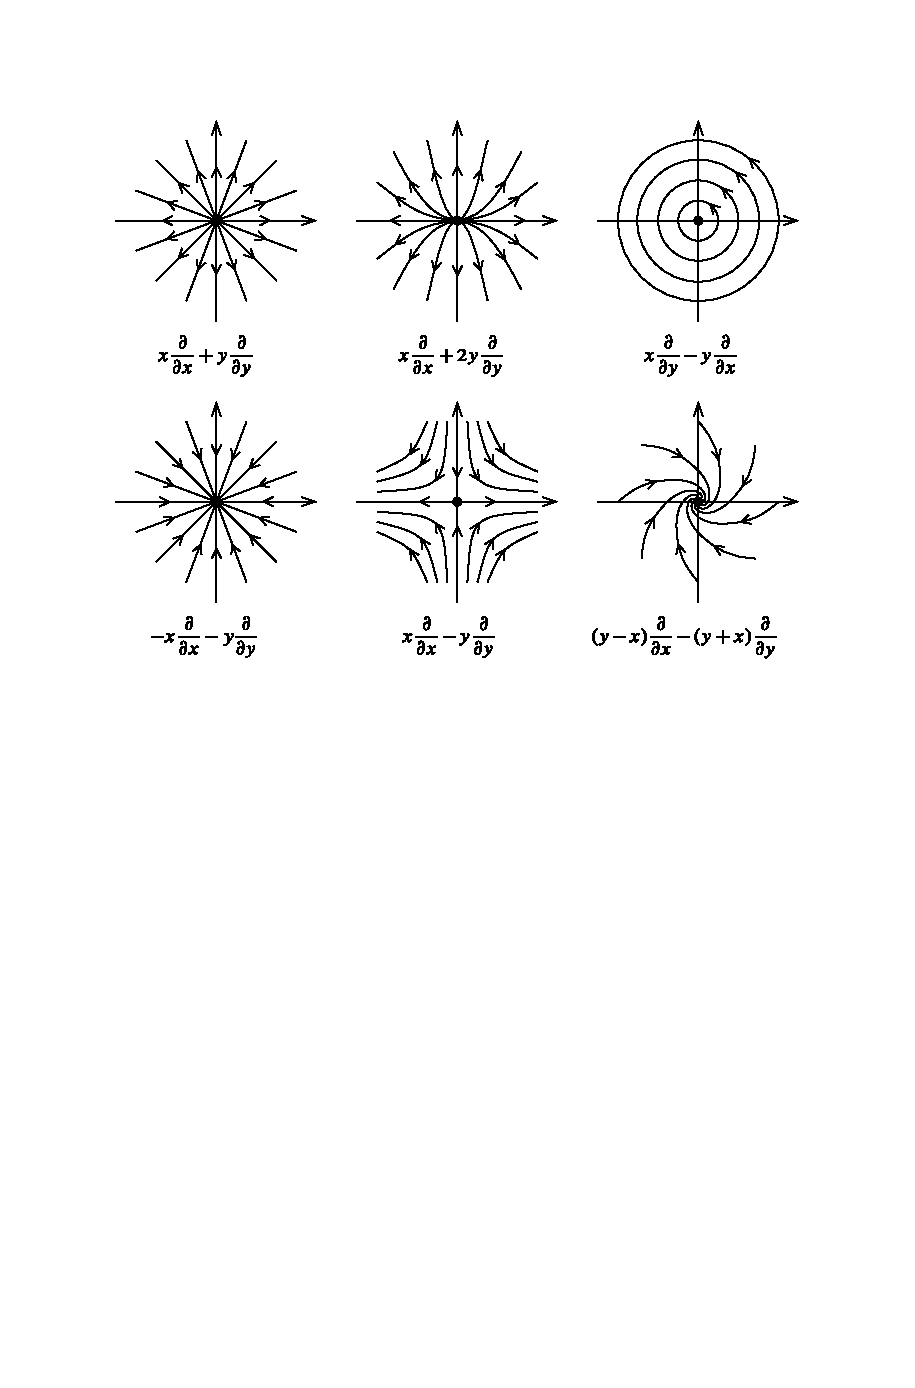
\includegraphics{pictures/equilibrium}
\caption{Examples of flows near equilibrium points.}
\label{equilibrium}
\end{figure}
The canonical form theorem shows that a flow in a neighborhood of a regular point behaves, up to diffeomorphism, just like translation along parallel coordinate
lines in $\R^n$. Thus all of the interesting local behavior of the flow is concentrated near its equilibrium points. The flow around equilibrium points can exhibit a wide variety of behaviors, such as closed orbits surrounding the equilibrium point, orbits converging to the equilibrium point as $t\to+\infty$ or $-\infty$, and many more complicated phenomena. Some typical $2$-dimensional examples are illustrated in Figure~\ref{equilibrium}.
\subsection{Flows and flowouts on manifolds with boundary}
On a manifold with boundary, the definitions of flow domain, flow, and infinitesimal generator of a flow are exactly the same as on a manifold without boundary. In general, a smooth vector field on a manifold with boundary need not generate a flow, because, for example, the integral curves starting at some boundary points might be defined only on half-open intervals. But there is a variant of the flowout theorem for manifolds with boundary, which has many important applications.\par
Suppose $M$ is a smooth manifold with nonempty boundary. The next theorem
describes a sort of \textit{one-sided flowout} from $\partial M$ determined by a vector field that is inward pointing everywhere on $\partial M$.
\begin{theorem}[\textbf{Boundary Flowout Theorem}]\label{flowout boundary}
Let $M$ be a smooth manifold with nonempty boundary, and let $N$ be a smooth vector field on $M$ that is inward-pointing at each point of $\partial M$. There exist a smooth function $\delta:\partial M\to\R^+$ and a smooth embedding $\varPsi:\mathcal{P}_\delta\to M$ where 
\[\mathcal{P}_\delta=\{(t,p):p\in\partial M,0\leq t<\delta(p)\}\sub\R\times\partial M\] 
such that $\varPhi(\mathcal{P}_\delta)$ is a neighborhood of $\partial M$, and for each $p\in\partial M$ the map $t\mapsto \varPsi(t,p)$ is an integral curve of $N$ starting at $p$.
\end{theorem}
\begin{proof}
We can define a flow in the same way as the flow theorem, but the domain is now not open. For every $p\in\partial M$, $\theta^{(p)}$ is a curve starting at $p$ point into $M$. Let $f(p)$ be the first time that $\theta^{(p)}$ hits the boundary again, and define $\delta(p)=f(p)/2$. Then we can define $\mathcal{P}_\delta$, and it is easy to see $\varPhi$ is an immersion. Assume $\varPhi(t,p)=\varPhi(t',p')$ with $(t,p),(t',p')\in\mathcal{P}_\delta$. Let's assume $t\leq t'$, then from $\theta_{t}(p)=\theta_{t'}(p')$ and the group law, we obtain
\[\theta_{t'-t}(p')=p\in\partial M\]
But $t'-t\leq t'<\delta(p')<f(p')$, this contradicts our definition. Thus $\varPhi$ is an injective immersion. Since $\partial M$ has dimension $(n-1)$, it is in fact an embedding.
\end{proof}
Let $M$ be a smooth manifold with boundary. A neighborhood of $\partial M$ is called a \textbf{collar neighborhood} if it is the image of a smooth embedding $[0,1)\times\partial M\to M$ that restricts to the obvious identification $\{0\}\times\partial M\to\partial M$.
\begin{theorem}[\textbf{Collar Neighborhood Theorem}]\label{collar nbhd}
If $M$ is a smooth manifold with nonempty boundary, then $\partial M$ has a collar neighborhood.
\end{theorem}
\begin{figure}[htbp]
\centering
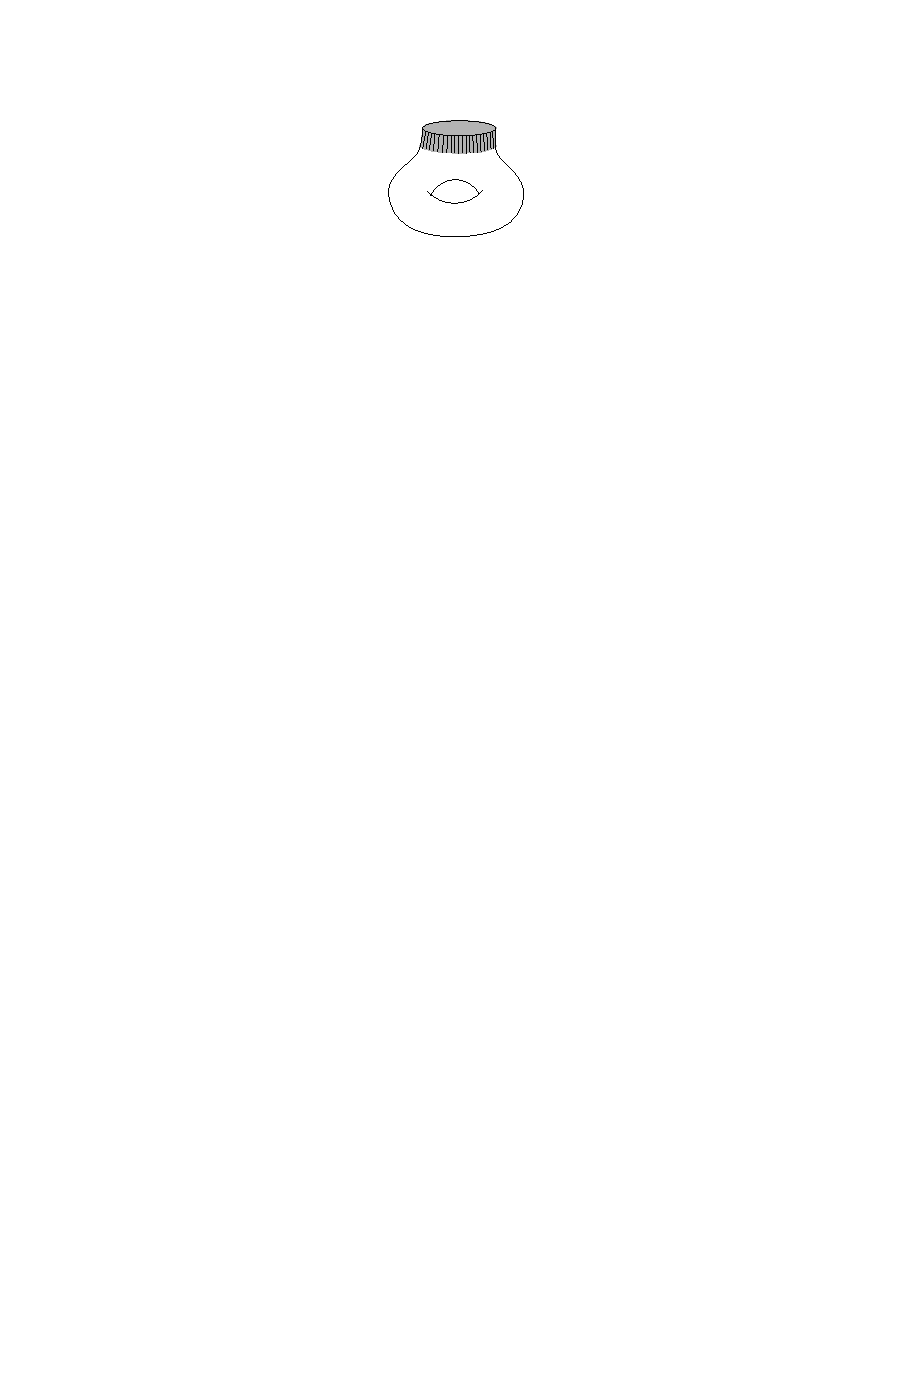
\includegraphics{pictures/collar}
\caption{A collar neighborhood of the boundary.}
\end{figure}
\begin{proof}
By the result of Exercise~\ref{vector field inward}, there exists a smooth vector field $N\in\X(M)$ whose restriction to $\partial M$ is everywhere inward-pointing. Let $\delta:M\to\R^+$ and $\varPhi:\mathcal{P}_\delta\to M$ be as in Theorem~\ref{flowout boundary}, and define a map $\psi:[0,1)\times\partial M\to\mathcal{P}_\delta$ by $\psi(t,p)=(t\delta(p),p)$. Then is a diffeomorphism that restricts to the identity on $\{0\}\times\partial M$ and therefore the map $\varPhi\circ\psi:[0,1)\times\partial M\to M$ is a smooth embedding with open image that restricts to the usual usual identification $\{0\}\times\partial M\to \partial M$. The image of $\varPhi\circ\psi$ is a collar neighborhood of $\partial M$.
\end{proof}
Our first application of the collar neighborhood theorem shows (among other things) that every smooth manifold with boundary is homotopy equivalent to its
interior.
\begin{theorem}\label{homotopy equiv Int M to M}
Let $M$ be a smooth manifold with nonempty boundary, and let $\iota:\Int M\hookrightarrow M$ denote inclusion. There exists a proper smooth embedding $R:M\to\Int M$ such that both $\iota\circ R:M\to M$ and $R\circ\iota:\Int M\to\Int M$ are smoothly homotopic to identity maps. Therefore, $\iota$ is a homotopy equivalence.
\end{theorem}
\begin{proof}
Theorem~\ref{collar nbhd} shows that $\partial M$ has a collar neighborhood $C_0$ in $M$, which is the image of a smooth embedding $E_0:[0,1)\times\partial M\to M$ satisfying $E_0(0,x)=x$ for all $x\in\partial M$. Let $f:M\to\R^+$ be a smooth positive exhaustion function. Note that 
\[W=\{(t,x):f(E_0(t,x))>f(x)-1\}\sub [0,1)\times\partial M\] 
is an open subset containing $\{0\}\times\partial M$. Using a partition of unity as in the proof of Theorem~\ref{flowout}, we may construct a smooth positive function $\delta:\partial M\to\R^+$ such that $(t,x)\in W$ whenever $0\leq t<\delta(x)$. Define 
\[E:[0,1)\times\partial M\to M,\quad E(t,x)=E_0(t\delta(x),x).\] 
Then $E$ is a diffeomorphism onto a collar neighborhood $C$ of $\partial M$, and by construction 
\[f(E(t,x))>f(x)-1\quad\text{for all }(t,x)\in[0,1)\times\partial M.\] 
We claim that for each $a\in(0,1)$, the set $E([0,a]\times\partial M)$ is closed in $M$: let $p$ be a limit point of $E([0,a]\times\partial M)$ in $M$, then there is a sequence $\{(t_i,x_i)\}$ in $[0,a]\times\partial M$ such that $E(t_i,x_i)\to p$. Then $f(E(t_i,x_i))$ remains bounded, and thus $f(x_i)<f(E(t_i,x_i))+1$ also remains bounded. Since $\partial M$ is closed in $M$, $f|_{\partial M}$ is also an exhaustion function, and therefore the sequence $\{x_i\}$ lies in some compact subset $K$ of $\partial M$. But then $(t_i,x_i)$ is contained in the compact subset $[0,a]\times K$, so by passing to a subsequence, we may assume $(t_i,x_i)\to(t_0,x_0)$. Therefore, $p=E(t_0,x_0)\in E([0,a]\times\partial M)$, implying $E([0,a]\times\partial M)$ is closed.\par
To simplify notation, we will use this embedding to identify $C$ with $[0,1)\times\partial M$ and denote a point in $C$ as an ordered pair $(s,x)$, with $s\in[0,1)$ and $x\in\partial M$; thus $(s,x)\in\partial M$ if and only if $s=0$. For any $a\in(0,1]$, let 
\[C(a)=\{(s,x)\in C:0\leq s<a\}=E([0,a)\times\partial M)\And M(a)=M-C(a)\]
To see that $M(a)$ is a regular domain, note first that it is closed in $M$ because it is the complement of the open set $C(a)$. Let $p\in M(a)$ be arbitrary. If $p\notin E([0,a]\times\partial M)$, then $p$ has a neighborhood in $\Int M$ contained in $M(a)$ by the argument above. If $p\in E([0,a]\times\partial M)$, then $p=E(a,x)$ for some $x\in\partial M$. Let $U$ be  a smooth chart of $x$, then $E([a,1)\times U)$ is a slice boundary chart for $p$. This proves $M(a)$ is a properly embedded submanifold.\par
Let $\psi:[0,1)\to [1/3,1)$ be an increasing diffeomorphism that satisfies $\psi(s)=s$ for $2/3\leq s<1$, and define $R:M\to\Int M$ by
\[R(p)=\begin{cases}
p,&p\in\Int(M(2/3));\\
(\psi(s),x),&p=(s,x)\in C.
\end{cases}\]
These definitions both give the identity map on the set $C-C(2/3)$ where they overlap, so $R$ is smooth by the gluing lemma. It is a diffeomorphism onto the closed subset $M(1/3)$, so it is a proper smooth embedding of $M$ into $\Int M$.\par
Define $H:M\times I\to M$ by
\[H(p,t)=\begin{cases}
p,&p\in\Int(M(2/3));\\
\big(ts+(1-t)\psi(s),x\big),&p=(s,x)\in C
\end{cases}\]
As before, $H$ is smooth, and a straightforward verification shows that it is a homotopy from $\iota\circ R$ to $\mathrm{id}_M$. If $p\in\Int M$, then $H(p,t)=p$ for all $t\in I$, so the restriction of $H$ to $(\Int M)\times $ is a smooth homotopy from $R\circ\iota$ to $\mathrm{id}_{\Int M}$.
\end{proof}
Theorem~\ref{homotopy equiv Int M to M} is the main ingredient in the following generalization of the Whitney approximation theorem.
\begin{theorem}[\textbf{Whitney Approximation for Manifolds with Boundary}]
If $M$ and $N$ are smooth manifolds with boundary, then every continuous map from $M$ to $N$ is homotopic to a smooth map.
\end{theorem}
\begin{proof}
Theorem~\ref{Whitney appox-1} takes care of the case in which $\partial N=\emp$, so we may assume that $\partial N\neq\emp$. Let $F:M\to N$ be a continuous map, let $\iota:\Int N\to N$ be inclusion, and let $R:M\to\Int M$ be the map constructed in Theorem~\ref{homotopy equiv Int M to M}, so that $\iota\circ R:N\to N$ is smoothly homotopic to $\mathrm{id}_N$. Theorem~\ref{homotopy equiv Int M to M} shows that $R\circ F:M\to\Int N$ is homotopic to a smooth map $G$. It follows that 
\[\iota\circ G\simeq \iota\circ R\circ F\simeq F\]
so $\iota\circ G:M\to N$ is a smooth map homotopic to $F$.
\end{proof}
The next theorem generalizes the main result of Theorem~\ref{homotopy to smooth} to the case of maps into a manifold with boundary.
\begin{theorem}\label{homotopy smooth boundary}
Suppose $M$ and $N$ are smooth manifolds with or without boundary. If $F:M\to N$ are homotopic smooth maps, then they are smoothly homotopic.
\end{theorem}
\begin{proof}
Theorem~\ref{homotopy to smooth} takes care of the case $\partial N=\emp$, so we may assume that $N$ has nonempty boundary. Let $\iota:\Int N\to N$ and $R:N\to\Int N$ be as in Theorem~\ref{homotopy equiv Int M to M}. Then $R\circ F$ and $R\circ G$ are homotopic smooth maps from $M$ to $\Int N$, so Theorem~\ref{homotopy to smooth} shows that they are smoothly homotopic to each other. Thus we have smooth homotopies
\[F\simeq\iota\circ R\circ F\simeq\iota\circ R\circ G\simeq G\]
By transitivity of smooth homotopy, it follows that $F$ is smoothly homotopic to $G$.
\end{proof}
The following theorem is probably the most important application of the collar
neighborhood theorem.
\begin{theorem}[\textbf{Attaching Smooth Manifolds Along Boundaries}]\label{attach mani}
Let $M$ and $N$ be smooth $n$-manifolds with nonempty boundaries, and suppose $h:\partial N\to\partial M$ is a diffeomorphism. Let $M\cup_hN$ be the adjunction space formed by identifying each $x\in\partial N$ with $h(x)\in\partial M$. Then $M\cup_hN$ is a topological manifold without boundary, and has a smooth structure such that there are regular domains $M',N'\sub M\cup_hN$ diffeomorphic to $M$ and $N$, respectively, and satisfying 
\begin{align}\label{attach mani-1}
M'\cup N'=M\cup_hN,\quad M'\cap N'=\partial M=\partial N
\end{align}
If $M$ and $N$ are both compact, then $M\cup_hN$ is compact, and if they are both
connected, then $M\cup_hN$ is connected.
\end{theorem}
\begin{proof}
For simplicity, let $X=M\cup_hN$ denote the quotient space and $\pi:M\amalg N$ the quotient map. Let $V\sub M$ and $W\sub N$ be collar neighborhoods of $\partial M$ and $\partial N$, respectively, and denote the corresponding diffeomorphisms by 
\[\alpha:[0,1)\times\partial M\to V\And\beta:[0,1)\times\partial N\to W.\] 
Define a continuous map $\varPhi:V\amalg W\to(-1,1)\times\partial M$ by
\[\varPhi(x)=\begin{cases}
(-t,p),&x=\alpha(t,p)\in V;\\
(t,h(q)),&x=\beta(t,q)\in W.
\end{cases}\]
Then the restriction of $\varPhi$ to $V$ or $W$ is a topological embedding with closed image, from which it follows easily that $\varPhi$ is a closed map. Because $\varPhi$ is constant on the fibers of $\pi$, it descends to a continuous map $\widetilde{\varPhi}:\pi(V\amalg W)\to(-1,1)\times\partial M$. This map is bijective, and it is a homeomorphism because it too is a closed map: if $K\sub\pi(V\amalg W)$ is closed, then $\pi^{-1}(K)$ is closed in $V\amalg W$, and therefore $\widetilde{\varPhi}(K)=\varPhi(\pi^{-1}(K))$ is closed. Thus, $\pi(V\amalg W)$ is a topological $n$-manifold. On the other hand, the restriction of $\pi$ to the saturated open subset $\Int M\amalg\Int N$ is an injective quotient map and thus a homeomorphism onto its image; this shows that $X$ is locally Euclidean of dimension $n$. Since $X$ is the union of the second-countable open subsets $\pi(\Int M\amalg\Int N)$ and $\pi(V\amalg W)$, it is second-countable. Any two fibers in $M\amalg N$ can be separated by saturated open subsets, so $X$ is Hausdorff. Thus it is a topological $n$-manifold.\par
We define a collection of charts on $X$ as follows:
\[\begin{array}{ll}
(\pi(U),\varphi\circ\pi^{-1}|_{\pi(U)}),&\text{for each smooth chart $(U,\varphi)$ for $\Int M$ or $\Int N$};\\
(\widetilde{\varPhi}^{-1}(U),\varphi\circ\widetilde{\varPhi}|_{\widetilde{\varPhi}^{-1}(U)}),&\text{for each smooth chart $(U,\varphi)$ for $(-1,1)\times\partial M$}.
\end{array}\]
These maps are compositions of homeomorphisms, so they define coordinate charts on $X$, and it is straightforward to check that they are all smoothly compatible and thus define a smooth structure on $X$. The restriction of $\pi$ to $M$ is continuous, closed, and injective, and thus it is a proper embedding. In terms of any of the smooth charts constructed above and corresponding charts on $M$, $\pi$ has a coordinate representation that is either an identity map or an inclusion map, so it is a smooth embedding, and its image $M'$ is therefore a regular domain in $X$. Similar considerations apply to $N$, and the relations $(\ref{attach mani-1})$ follow immediately from the definitions.\par
If $M$ and $N$ are compact, then $X$ is the union of the compact sets $M'$ and $N'$, so it is compact; and if they are connected, then $X$ is the union of the connected sets $M'$ and $N'$ with points of $\partial M'=\partial N'$in common, so it is connected.
\end{proof}
\begin{corollary}
Suppose $M$ and $N$ are smooth $n$-manifolds with boundary, $A\sub\partial M$ and $B\sub\partial N$ are nonempty subsets that are unions of components of the respective boundaries, and $h:B\to A$ is a diffeomorphism. Then $M\cup_hN$ is a topological manifold with boundary, and can be given a smooth structure such that $M$ and $N$ are diffeomorphic to regular domains in $M\cup_hN$.
\end{corollary}
\begin{example}[\textbf{Connected Sums}]
Let $M_1,M_2$ be connected smooth manifolds of dimension $n$. For $i=1,2$, let $U_i$ be a regular coordinate ball centered at some point $p_i\in M_i$, and let $M'_i=M_i-U_i$. Exercise~\ref{delete coordinate ball} shows that each $M'_i$ is a smooth manifold with boundary whose boundary is diffeomorphic to $S^{n-1}$. A smooth connected sum of $M_1$ and $M_2$, denoted by $M_1\#M_2$, is a smooth manifold formed by choosing a diffeomorphism from $\partial M_1$ to $\partial M_2$ and attaching $M'_1$ and $M'_2$ along their boundaries.
\end{example}
If $M$ is any smooth manifold with boundary, Theorem~\ref{homotopy equiv Int M to M} shows that $M$ can be properly embedded into a smooth manifold without boundary (namely, a copy of $\Int M$). The next example shows a different way that $M$ can be so embedded; this construction has the advantage of embedding $M$ into a compact manifold when $M$ itself is compact.
\begin{example}[\textbf{The Double of a Smooth Manifold with Boundary}]\label{double manifold boundary}
Let $M$ be a smooth manifold with boundary. The \textbf{double of $\bm{M}$} is the manifold $D(M)=M\cup_{\mathrm{id}}M$, where $\mathrm{id}:\partial M\to\partial M$ is the identity map of $\partial M$, it is obtained from $M\amalg M$ by identifying each boundary point in one copy of $M$ with the same boundary point in the other. It is a smooth manifold without boundary, and contains two regular domains diffeomorphic to $M$. It is easy to check that $D(M)$ compact if and only if $M$ is compact, and connected if and only if $M$ is connected. $($It is useful to extend the definition to manifolds without boundary by defining $D(M)=M\amalg M$ when $\partial M=\emp$.$)$
\end{example}
Although vector fields on manifolds with boundary do not always generate flows,
there is one circumstance in which they do: when the vector field is everywhere
tangent to the boundary. To prove this, we begin with the following special case.
\begin{lemma}\label{flow tangent boundary}
Suppose $M$ is a smooth manifold and $D\sub M$ is a regular domain. If $V$ is a smooth vector field on $M$ that is tangent to $\partial D$, then every integral curve of $V$ that starts in $D$ remains in $D$ as long as it is defined.
\end{lemma}
\begin{proof}
Suppose $\gamma:J\to M$ is an integral curve of $V$ with $\gamma(0)\in D$. Define $\mathcal{T}=\{t\in J:\gamma(t)\in D\}$. We will show that $\mathcal{T}$ is both open and closed in $J$; since $J$ is an interval, this implies $\mathcal{T}=J$ and proves the lemma.\par
Since $D$ is closed in $M$ (by definition of a regular domain), $\mathcal{D}$ is closed in $J$ by continuity. To prove it is open, suppose $t_0\in\mathcal{T}$. If $\gamma(t_0)\in\Int D$, then a neighborhood of $t_0$ is contained in $\mathcal{T}$ by continuity, so we can assume $\gamma(t_0)\in\partial D$. Because $V$ is tangent to $\partial D$, Proposition~\ref{vector field restrict submani} shows that there is a smooth vector field $W=V|_{\partial D}$ that is $\iota$-related to $V$, where $\iota:\partial D\hookrightarrow M$ is inclusion. Let $\widetilde{\gamma}:(t_0-\eps,t_0+\eps)\to \partial D$ be an integral curve of $W$ with $\widetilde{\gamma}(t_0)=\gamma(t_0)$. By naturality of integral curves (Proposition~\ref{integral curve naturality}), $\iota\circ\widetilde{\gamma}$ is an integral curve of $V$ with the same initial condition, so by uniqueness it must be equal to $\gamma$ where both are defined. This shows that $\gamma(t)\sub \partial D\sub D$ for $t$ in some neighborhood of $t_0$, so $\mathcal{T}$ is open in $J$ as claimed.
\end{proof}
\begin{theorem}[\textbf{Flows on Manifolds with Boundary}]\label{flow boundary}
The conclusions of Theorem~\ref{flow fundamental thm} remain true if $M$ is a smooth manifold with boundary and $V$ is a smooth vector field on $M$ that is tangent to $\partial M$.
\end{theorem}
\begin{proof}
We can consider $M$ as a regular domain in its double $D(M)$. By the extension lemma for vector fields, we can extend $V$ to a smooth vector field $\widetilde{V}$ on $D(M)$. Let $\widetilde{\theta}:\mathcal{D}\to D(M)$ be the flow of $\widetilde{V}$, and let $\mathcal{D}=(\R\times M)\cap \widetilde{\mathcal{D}}$ and $\theta=\widetilde{\theta}|_{M}$. Then Lemma~\ref{flow tangent boundary} guarantees that $\theta$ maps $\mathcal{D}$ into $M$, and the rest of the conclusions follow from Theorem~\ref{flow fundamental thm} applied to $\widetilde{V}$.
\end{proof}
For manifolds with boundary, the canonical form theorem has the following
variant.
\begin{theorem}[\textbf{Canonical Form Near a Regular Point on the Boundary}]
Let $M$ be a smooth manifold with boundary and let $V$ be a smooth vector field on $M$ that is tangent to $\partial M$. If $p\in\partial M$ is a regular point of $V$, there exist smooth boundary coordinates $(s^i)$ on some neighborhood of $p$ in which $V$ has the coordinate representation $\partial/\partial s^1$.
\end{theorem}
\subsection{Lie derivatives}
Suppose $M$ is a smooth manifold, $V$ is a smooth vector field on $M$, and $\theta$ is the flow of $V$. For any smooth vector field $W$ on $M$, define a rough vector field on $M$, denoted by $\mathfrak{L}_VW$ and called the Lie derivative of $W$ with respect to $V$, by
\[(\mathfrak{L}_VW)_p=\frac{d}{dt}\Big|_{t=0}d(\theta_{-t})_{\theta_t(p)}\big(W_{\theta_t(p)}\big)=\lim_{t\to 0}\frac{d(\theta_{-t})_{\theta_t(p)}\big(W_{\theta_t(p)}\big)-W_p}{t}\]
provided the derivative exists. For small $t\neq 0$, at least the difference quotient makes sense: $\theta_t$ is defined in a neighborhood of $p$, and $\theta_{-t}$ is the inverse of $\theta_t$, so both $d(\theta_{-t})_{\theta_t(p)}\big(W_{\theta_t(p)}\big)$ and $W_p$ are elements of $T_pM$.
\begin{figure}[htbp]
\centering
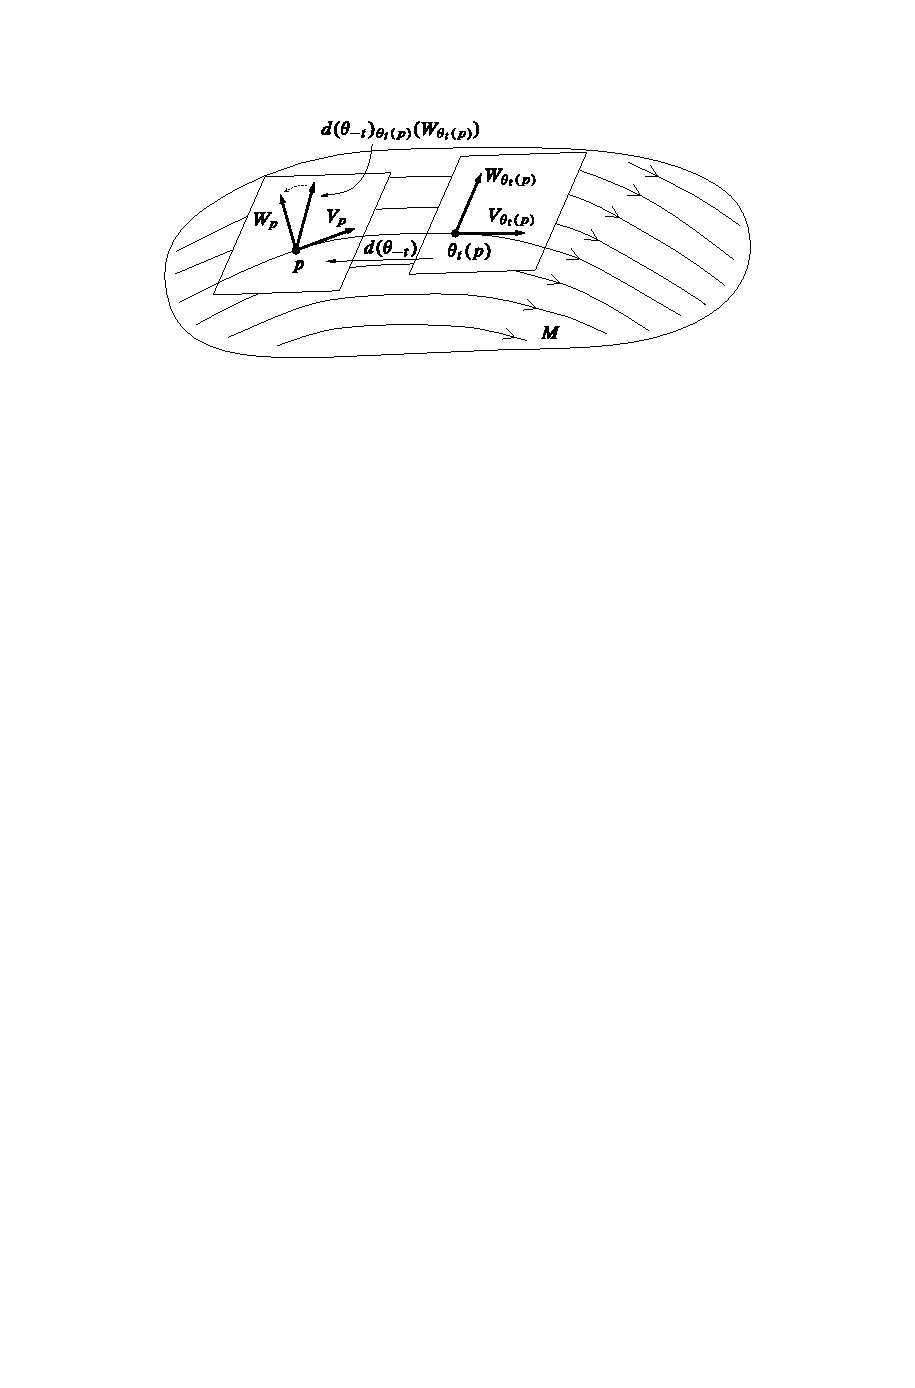
\includegraphics{pictures/Lie-derivative}
\caption{The Lie derivative of a vector field.}
\end{figure}\par
If $M$ has nonempty boundary, this definition of $\mathfrak{L}_VW$ makes sense as long as $V$ is tangent to $\partial M$ so that its flow exists by Theorem~\ref{flow boundary}.
\begin{lemma}\label{Lie derivative exist}
Suppose $M$ is a smooth manifold with or without boundary, and $V,W\in\X(M)$. If $\partial M\neq\emp$, assume in addition that $V$ is tangent to $\partial M$. Then $(\mathfrak{L}_VW)_p$ exists for every $p\in M$, and $\mathfrak{L}_VW$ is a smooth vector field.
\end{lemma}
\begin{proof}
Let $\theta$ be the flow of $V$. For arbitrary $p\in M$, let $(U,(x^i))$ be a smooth chart containing $p$. Choose an open interval $J_0$ containing $0$ and an open subset $U_0\sub U$ containing $p$ such that$\theta$ maps $J_0\times U_0$ into $U$. For $(t,x)\in J_0\times U_0$, write the component functions of $\theta$ as $(\theta^1(t,x),\dots,\theta^n(t,x))$. Then for any $(t,x)\in J_0\times U_0$,
the matrix of $d(\theta_{-t})_{\theta_t(p)}:T_{\theta_t(x)}M\to T_xM$ is
\[\begin{pmatrix}
\dfrac{\partial\theta^i}{\partial x^j}(-t,\theta_t(x))
\end{pmatrix}\]
Therefore,
\[d(\theta_{-t})_{\theta_t(p)}\big(W_{\theta_t(p)}\big)=\dfrac{\partial\theta^i}{\partial x^j}(-t,\theta_t(x))W^j(\theta_t(x))\frac{\partial}{\partial x^i}\Big|_x\]
Because $\theta^i$ and $W^j$ are smooth functions, the coefficient of $\partial/\partial x^i|_x$ depends smoothly on $(t,x)$. It follows that $(\mathfrak{L}_VW)_x$, which is obtained by taking the derivative of this expression with respect to $t$ and setting $t=0$, exists for each $x\in U_0$ and
depends smoothly on $x$.
\end{proof}
The definition of $\mathfrak{L}_VW$ is not very useful for computations, because typically the flow is difficult or impossible to write down explicitly. Fortunately, there is a simple formula for computing the Lie derivative without explicitly finding the flow.
\begin{theorem}\label{Lie derivative bracket}
If $M$ is a smooth manifold and $V,W\in\X(M)$, then $\mathfrak{L}_VW=[V,W]$.
\end{theorem}
\begin{proof}
Suppose $V,W\in\X(M)$, and let $\mathcal{R}(V)\sub M$ be the set of regular points of $V$ (the set of points $p\in M$ such that $V_p\neq0$). Note that $\mathcal{R}(V)$ is open in $M$ by continuity, and its closure is the support of $V$. We will show that $(\mathfrak{L}_VW)_p=[V,W]_p$ for all $p\in M$, by considering three cases.\par
First let $p\in\mathcal{R}(V)$. In this case, we can choose smooth coordinates $(u^i)$ on a neighborhood of $p$ in which $V$ has the coordinate representation $V=\partial/\partial u^i$ (Theorem~\ref{flow canonical form}). In these coordinates, the flow of $V$ is $\theta_t(u)=(u^1+t,u^2,\dots,u^n)$. For each fixed $t$, the matrix of $d(\theta_{-t})_{\theta_t(x)}$ in these coordinates is the identity at every point. Consequently, for any $u\in U$,
\begin{align*}
d(\theta_{-t})_{\theta_t(p)}\big(W_{\theta_t(p)}\big)&=d(\theta_{-t})_{\theta_t(p)}\Big(W^j(u^1+t,u^2,\dots,u^n)\frac{\partial}{\partial u^j}\Big|_{\theta_t(u)}\Big)\\
&=W^j(u^1+t,u^2,\dots,u^n)\frac{\partial}{\partial u^j}\Big|_{u}
\end{align*}
Using the definition of the Lie derivative, we obtain
\[(\mathfrak{L}_VW)_u=\frac{d}{dt}\Big|_{t=0}W^j(u^1+t,u^2,\dots,u^n)\frac{\partial}{\partial u^j}\Big|_{u}=\frac{\partial W^j}{\partial u^1}(u^1,\dots,u^n)\frac{\partial}{\partial u^j}\Big|_u\]
On the other hand, by virtue of formula $(\ref{Lie bracket-1})$ for the Lie bracket in coordinates, $[V,W]_u$ is easily seen to be equal to the same expression.\par
Now let $p\in\supp(V)$. Because $\supp(V)$ is the closure of $\mathcal{R}(V)$, it follows by continuity that $(\mathfrak{L}_VW)_p=[V,W]_p$ for $p\in\supp(V)$.\par
Finally, let $p\in M\setminus\supp(V)$. In this case, $V\equiv 0$ on a neighborhood of $p$. On the one hand, this implies that $\theta_t$ is equal to the identity map in a neighborhood of $p$ for all $t$, so $d(\theta_{-t})_{\theta_t(p)}\big(W_{\theta_t(p)}\big)=W_p$, which implies $(\mathfrak{L}_VW)_p=0$. On the other hand, $[V,W]=0$ by formula $(\ref{Lie bracket-1})$.
\end{proof}
This theorem allows us to extend the definition of the Lie derivative to arbitrary
smooth vector fields on a smooth manifold $M$ with boundary. Given $V,W\in\X(M)$, we define $(\mathfrak{L}_VW)_p$ for $p\in\partial M$ by embedding $M$ in a smooth manifold $\widetilde{M}$ without boundary (such as the double of $M$), extending $V$ and $W$ to smooth vector fields on $\widetilde{M}$, and computing the Lie derivative there. By virtue of the preceding theorem, $(\mathfrak{L}_VW)_p=[V,W]_p$ is independent of the choice of extension.\par
Theorem~\ref{Lie derivative bracket} also gives us a geometric interpretation of the Lie bracket of two vector fields: it is the directional derivative of the second vector field along the flow of the first. A number of nonobvious properties of the Lie derivative follow immediately from things we already know about Lie brackets.
\begin{corollary}
Suppose $M$ is a smooth manifold with or without boundary, and $V,W,X\in\X(M)$.
\begin{itemize}
\item[(a)] $\mathfrak{L}_VW=-\mathfrak{L}_WV$.
\item[(b)] $\mathfrak{L}_V[W,X]=[\mathfrak{L}_VW,X]+[W,\mathfrak{L}_VX]$.
\item[(c)] $\mathfrak{L}_{[V,W]}X=\mathfrak{L}_V\mathfrak{L}_WX-\mathfrak{L}_W\mathfrak{L}_VX$.
\item[$(d)$] If $g\in C^\infty(M)$, then $\mathfrak{L}_V(gW)=(Vg)W+g\mathfrak{L}_VW$.
\item[$(e)$] If $F:M\to N$ is a diffeomorphism, then $F_*(\mathfrak{L}_VX)=\mathfrak{L}_{F_*V}F_*X$.
\end{itemize}
\end{corollary}
\begin{proof}
Recall the Jacobi identity
\[[V,[W,X]]+[W,[X,V]]+[X,[V,W]]=0\]
Thus
\begin{align*}
\mathfrak{L}_V[W,X]&=[V,[W,X]]=-[W,[X,V]]-[X,[V,W]]\\
&=[[V,W],X]+[W,[V,X]]\\
&=[\mathfrak{L}_VW,X]+[W,\mathfrak{L}_VX]
\end{align*}
Similarly,
\begin{align*}
\mathfrak{L}_{[V,W]}X&=[[V,W],X]=[V,[W,X]]+[W,[X,V]]\\
&=[V,[W,X]]-[W,[V,X]]\\
&=\mathfrak{L}_V[W,X]-\mathfrak{L}_W[V,X]\\
&=\mathfrak{L}_V\mathfrak{L}_WX-\mathfrak{L}_W\mathfrak{L}_VX
\end{align*}
Part $(d)$ is a direct computation:
\begin{align*}
\mathfrak{L}_V(gW)&=[V,gW]=V(gW)-gWV=(Vg)W+gVW-gWV\\
&=(Vg)W+g[V,W]=(Vg)W+g\mathfrak{L}_VW
\end{align*}
and the last statment is a result of natruality of Lie bracket.
\end{proof}
Part $(d)$ of this corollary gives a meaning to the mysterious formula $(\ref{Lie bracket two product rule})$ for Lie brackets of vector fields multiplied by functions: because the Lie bracket $[fV,gW]$ can be thought of as the Lie derivative $\mathfrak{L}_{fV}(gW)$, it satisfies a product rule in $g$ and $W$, and because it can also be thought of as $-\mathfrak{L}_{gW}(fV)$, it satisfies a product
rule in $f$ and $V$ as well. Expanding out these two product rules yields $(\ref{Lie bracket two product rule})$:
\begin{align*}
\mathfrak{L}_{fV}(gW)&=(fVg)W+g\mathfrak{L}_{fV}W=(fVg)W-g\mathfrak{L}_{W}(fV)\\
&=(fVg)W-g(Wf+f\mathfrak{L}_{W}V)\\
&=(fVg)W-(gWf)+fg\mathfrak{L}_VW
\end{align*}
If $V$ and $W$ are vector fields on $M$ and $\theta$ is the flow of $V$, the Lie derivative $(\mathfrak{L}_VW)_p$, by definition, expresses the $t$-derivative of the time-dependent vector $d(\theta_{-t})_{\theta_t(p)}\big(W_{\theta_t(p)}\big)$ at $t=0$. The next proposition shows how it can also be used to compute the derivative of this expression at other times.
\begin{proposition}\label{Lie derivative t_0}
Suppose $M$ is a smooth manifold with or without boundary and $V,W\in\X(M)$. If $\partial M\neq\emp$, assume also that $V$ is tangent to $\partial M$. Let $\theta$ be the flow of $V$. For any $(t_0,p)$ in the domain of $\theta$,
\begin{align*}
\frac{d}{dt}\Big|_{t=t_0}d(\theta_{-t})_{\theta_t(p)}\big(W_{\theta_t(p)}\big)=d(\theta_{-t_0})\big((\mathfrak{L}_VW)_{\theta_{t_0}(p)}\big)
\end{align*}
\end{proposition}
\begin{figure}[htbp]
\centering
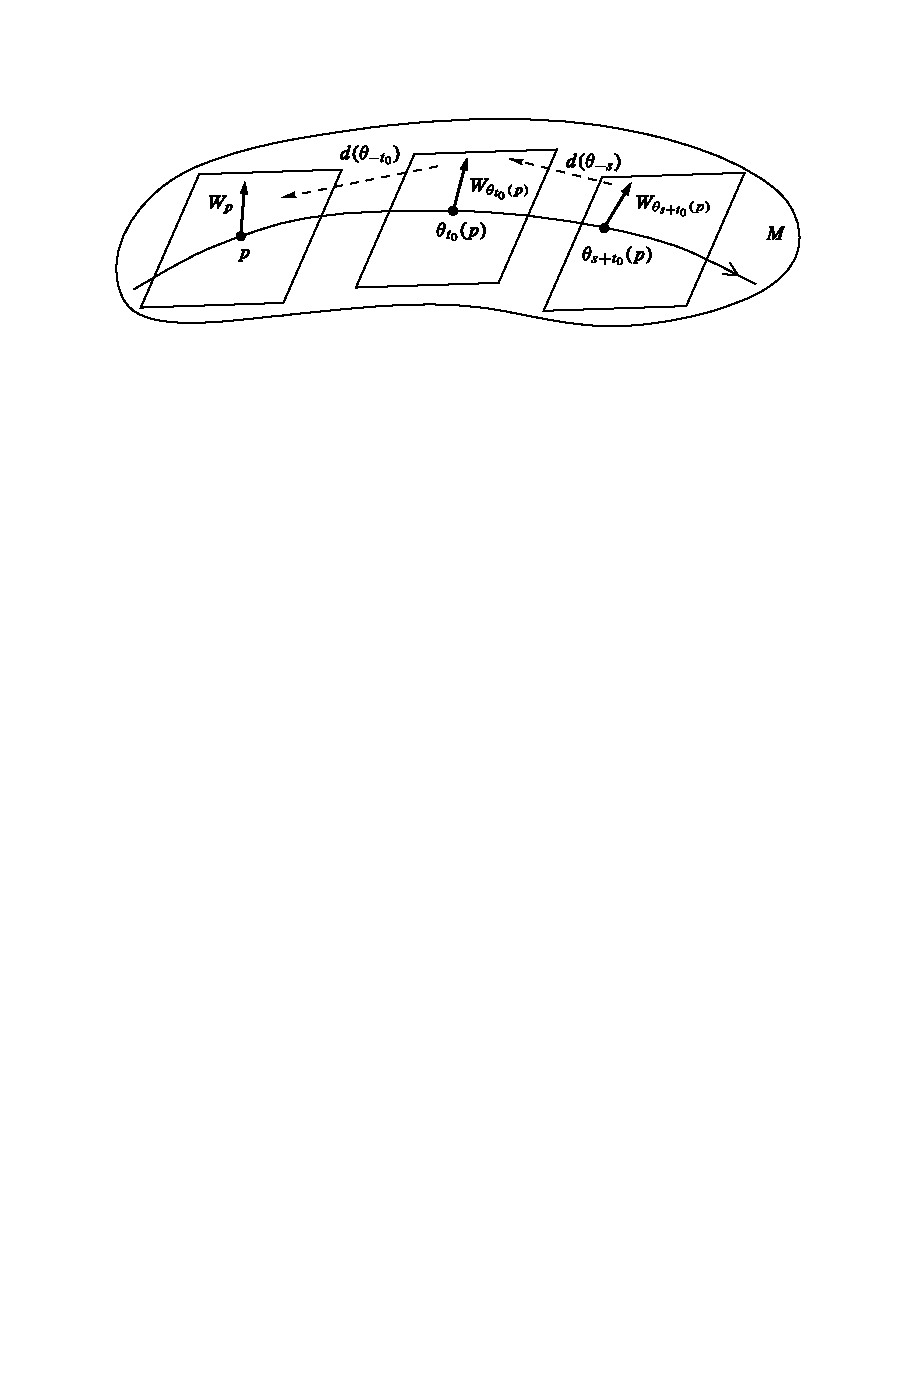
\includegraphics{pictures/Lie-derivative-2}
\caption{Proof of Proposition~\ref{Lie derivative t_0}.}
\end{figure}
\begin{proof}
Let $p\in M$ be arbitrary, let $\mathcal{D}^{(p)}\sub\R$ denote the domain of the integral curve $\theta^{(p)}$, and consider the map $X:\mathcal{D}^{(p)}\to T_pM$ given by $X(t)=d(\theta_{-t})_{\theta_t(p)}\big(W_{\theta_t(p)}\big)$. The argument in the proof of Lemma~\ref{Lie derivative exist} shows that $X$ is a smooth curve in the vector space $T_pM$. Making the change of variables $t=t_0+s$ we obtain
\begin{align*}
X'(t_0)&=\frac{d}{dt}\Big|_{s=0}X(t_0+s)=\frac{d}{dt}\Big|_{s=0}d(\theta_{-t_0-s})(W_{\theta_{s+t_0}(p)})\\
&=\frac{d}{dt}\Big|_{s=0}d(\theta_{-t_0})\circ d(\theta_{-s})(W_{\theta_{s}\circ\theta_{t_0}(p)})\\
&=d(\theta_{-t_0})\frac{d}{dt}\Big|_{s=0}d(\theta_{-s})(W_{\theta_{s}\circ\theta_{t_0}(p)})\\
&=d(\theta_{-t_0})\big((\mathfrak{L}_VW)_{\theta_{t_0}(p)}\big)
\end{align*}
as needed.
\end{proof}
\subsection{Commuting vector fields}
Let M be a smooth manifold and $V,W\in\X(M)$. We say that $V$ and $W$ \textbf{commute} if $VWf=WVf$ for every smooth function $f$, or equivalently if $[V,W]\equiv0$. If $\theta$ is a smooth flow, a vector field $W$ is said to be invariant under $\theta$ if $W$ is $\theta_t$-related to itself for each $t$; more precisely, this means that $W|_{M_t}$ is $\theta_t$-related for each $t$, or equivalently that $d(\theta_t)_p(W_p)=W_{\theta_t(p)}$ for all $(t,p)$ in the domain of $\theta$. The next proposition shows that these two concepts are intimately related.
\begin{theorem}\label{vector field commute iff}
For smooth vector fields $V$ and $W$ on a smooth manifold $M$, the following are equivalent:
\begin{itemize}
\item[(a)] $V$ and $W$ commute.
\item[(b)] $W$ is invariant under the flow of $V$.
\item[(c)] $V$ is invariant under the flow of $W$.
\end{itemize}
\end{theorem}
\begin{proof}
Suppose $V,W\in\X(M)$, and let $\theta$ denote the flow of $V$. If (b) holds, then $d(\theta_t)_p(W_p)=W_{\theta_t(p)}$ whenever $(t,p)$ is in the domain of $\theta$. Applying $d(\theta_{-t})_{\theta_t(p)}$ to both sides, we conclude that $d(\theta_{-t})_{\theta_t(p)}(W_{\theta_t(p)})=W_p$, which obviously implies $\mathfrak{L}_VW=[V,W]=0$ directly from the definition of the Lie derivative. The same argument shows that (c) implies (a).\par
To prove that (a) implies (b), assume that $[V,W]=\mathfrak{L}_VW=0$. Let $p\in M$ be arbitrary, and let $X(t)=d(\theta_{-t})_{\theta_t(p)}\big(W_{\theta_t(p)}\big)$ for $t\in\mathcal{D}^{(p)}$. Proposition~\ref{Lie derivative t_0} shows that $X'(t)\equiv 0$. Since $X(0)=W_p$, this implies that $X(t)\equiv W_p$ for all $t\in\mathcal{D}^{(p)}$, and applying $d(\theta_t)_p$ to both sides yields the identity that says $W$ is invariant under $\theta$. The same proof also shows that (a) implies (c).
\end{proof}
\begin{corollary}
Every smooth vector field is invariant under its own flow.
\end{corollary}
\begin{proof}
Use the preceding proposition together with the fact that $[V,V]\equiv 0$.
\end{proof}
The deepest characterization of commuting vector fields is in terms of the relationship between their respective flows. The next theorem says that two vector fields
commute if and only if their flows commute. But before we state the theorem formally, we need to examine exactly what this means. Suppose $V$ and $W$ are smooth vector fields on $M$, and let $\theta$ and denote their respective flows. If $V$ and $W$ are complete, it is clear what we should mean by saying their flows commute: simply that $\theta_t\circ\psi_s=\psi_s\circ\theta_t$ for all $s,t\in\R$. However, if either $V$ or $W$ is not complete, the most we can hope for is that this equation holds for all $s$ and $t$ such that both sides are defined. Unfortunately, even when the vector fields commute, their flows might not commute in this naive sense, because there are examples of commuting vector fields $V$ and $W$ and particular choices of $t$, $s$, and $p$ for which both $\theta_t\circ\psi_s(p)$ and $\psi_s\circ\theta_t(p)$ are defined, but they are not equal. Here is the problem: if $\theta_t\circ\psi_s(p)$ is defined for $t=t_0$ and $s=s_0$, then by the properties of flow domains, it must be defined for all $t$ in some open interval containing $0$ and $t_0$, but the analogous statement need not be true of $s$---there might be values of $s$ between $0$ and $s_0$ for which the integral curve of $V$ starting at $\psi_s(p)$ does not extend all the way to $t=t_0$.\par
Thus we make the following definition. If $\theta$ and $\psi$ are flows on $M$, we say that $\theta$ and $\psi$ commute if the following condition holds for every $p\in M$, whenever $J$ and $K$ are open intervals containing $0$ such that one of the expressions $\theta_t\circ\psi_s(p)$ or $\psi_s\circ\theta_t(p)$ is defined for all $(t,s)\in J\times K$, both are defined and they are equal. For global flows, this is the same as saying that $\theta_t\circ\psi_s=\psi_s\circ\theta_t$ for all $s$ and $t$.
\begin{theorem}\label{vector filed commute flow}
Smooth vector fields commute if and only if their flows commute.
\end{theorem}
\begin{proof}
Let $V$ and $W$ be smooth vector fields on a smooth manifold $M$, and let $\theta$ and denote $\psi$ their respective flows. Assume first that $V$ and $W$ commute. Suppose that $p\in M$, and $J$ and $K$ are open intervals containing $0$ such that $\psi_s\circ\theta_t(p)$ is defined for all $(s,t)\in J\times K$. (The same proof with $V$ and $W$ reversed works under the assumption that the other expression is defined on such a rectangle.) By Theorem~\ref{vector field commute iff}, the hypothesis implies that $V$ is invariant under $\psi$. Fix any $s\in J$, and consider the curve $\gamma:K\to M$ defined by $\gamma(t)=\psi_s\circ\theta_t(p)=\psi_s(\theta^{(p)}(t))$. This curve satisfies $\gamma(0)=\psi_s(p)$, and its velocity at $t\in K$ is
\[\gamma'(t)=\frac{d}{dt}\big(\psi_s(\theta^{(p)}(t))\big)=d(\psi_s)(\dot{\theta}^{(p)}(t))=d(\psi_s)(V_{\theta^{(p)}(t)})=V_{\gamma(t)}\]
Thus, $\gamma$ is an integral curve of $V$ starting at $\psi_s(p)$. By uniqueness, therefore,
\[\gamma(t)==\theta^{(\psi_s(p))}(t)=\theta_t\big(\psi_s(p)\big)\]
This proves that $\theta$ and $\psi$ commute.\par
Conversely, assume that the flows commute, and let $p\in M$. If $\eps>0$ is chosen
small enough that $\psi_s\circ\theta_t(p)$ is defined whenever $|s|<\eps$ and $|t|<\eps$, then the hypothesis guarantees that $\psi_s\circ\theta_t(p)=\theta_t\circ\psi_s(p)$ for all such $s$ and $t$. This can be rewritten in the form
\[\psi^{(\theta_t(p))}(s)=\theta_t(\psi^{(p)}(s))\]
Differentiating this relation with respect to $s$, we get
\[W_{\theta_t(p)}=\frac{d}{ds}\Big|_{s=0}\psi^{(\theta_t(p))}(s)=\frac{d}{ds}\Big|_{s=0}\theta_t(\psi^{(p)}(s))=d(\theta_t)_p(W_p)\]
This means $W_p$ is invariant under $\theta_t$, thus by Theorem~~\ref{vector field commute iff} $V$ commutes with $W$.
\end{proof}
\subsubsection{Commuting frames}
Suppose $M$ is a smooth $n$-manifold. Recall that a local frame for $M$ is an $n$-tuple $(E_i)$ of vector fields defined on an open subset $U\sub M$ such that $(E_i|_p)$ forms a basis for $T_pM$ at each $p\in U$. A smooth local frame $(E_i)$ for $M$ is called a commuting frame if $[E_i,E_j]=0$ for all $i$ and $j$. 
\begin{example}[\textbf{Commuting and Noncommuting Frames}]\label{commute frame eg}
\mbox{}
\begin{itemize}
\item[(a)] The simplest examples of commuting frames are the coordinate frames. Given any smooth coordinate chart $(U,(x^i))$ for a smooth manifold $M$, $(\ref{Lie bracket-1})$ shows that the coordinate frame $(\partial/\partial x^i)$ is a commuting frame.
\item[(b)] The frame $(E_1,E_2)$ for $\R^2$ over $\R^2-\{0\}$ defined by $(\ref{polar frame R^2-1})$ is not a commuting frame, because a straightforward computation shows that
\[[E_1,E_2]=\frac{y}{r^2}\frac{\partial}{\partial x}-\frac{x}{r^2}\frac{\partial}{\partial y}\neq 0\]
\end{itemize}
\end{example}
Because every coordinate frame is a commuting frame, and because Lie brackets
are invariantly defined, it follows that a necessary condition for a smooth frame to be expressible as a coordinate frame in some smooth chart is that it be a commuting frame. Thus, the computation above shows that $(E_1,E_2)$ cannot be expressed as a coordinate frame for $\R^2$ with respect to any choice of smooth local coordinates.\par
The next theorem shows that commuting is also a sufficient condition for a smooth frame to be locally expressible as a coordinate frame.
\begin{theorem}[\textbf{Canonical Form for Commuting Vector Fields}]\label{flow commute canonical form}
Let $M$ be a smooth $n$-manifold, and let $(V_1,\dots,V_k)$ be a linearly independent $k$-tuple of smooth commuting vector fields on an open subset $W\sub M$. For each $p\in W$, there exists a smooth coordinate chart $(U,(s^i))$ centered at $p$ such that $V_i=\partial/\partial s^i$ for $1\leq i\leq k$. If $S\sub W$ is an embedded codimension-$k$ submanifold and $p$ is a point of $S$ such that $T_pS$ is complementary to the span of $(V_1|_p,\dots,V_k|_p)$, then the coordinates can also be chosen such that $S\cap U$ is the slice defined by $s^1=\cdots=s^k=0$.
\end{theorem}
\begin{proof}
Let $p\in W$ be arbitrary. If no submanifold $S$ is given, just let $S$ be any
smooth embedded codimension-$k$ submanifold $S$ whose tangent space at $p$ is complementary to the span of $(V_1|_p,\dots,V_k|_p)$ (e.g., an appropriate coordinate slice) Let $(U,(s^i))$ be a slice chart for $S$ centered at $p$, with $U\sub W$, and with $S\cap U$ equal to the slice $\{x\in U:x^1=\cdots=x^k=0\}$. Our assumptions ensure that the vectors $\{V_1|_p,\dots,V_k|_p,\partial/\partial x^{k+1}|_p,\dots,\partial/\partial x^n|_p\}$ span $T_pM$. Since the theorem is
purely local, we may as well consider $V_1,\dots,V_k$ as vector fields on $U\sub\R^n$, and consider $S$ to be the subset of $U$ where the first $k$ coordinates vanish. The basic idea of this proof is similar to that of the flowout theorem, except that we have to do a bit of extra work to make use of the hypothesis that the vector fields commute.\par
Let $\theta_i$ denote the flow of $V_i$ for $i=1,\dots,k$. There exist $\eps>0$ and a neighborhood $Y$ of $p$ in $U$ such that the composition $(\theta_1)_{t_1}\circ\cdots\circ(\theta_k)_{t_k}$ is defined on $Y$ and maps $Y$ into $U$ whenever $|t_1|,\dots,|t_k|$ are all less than $\eps$. (To see this, just choose $\eps_k>0$ and $U_k\sub U$ such that $\theta_k$ maps $(-\eps_k,\eps_k)\times U_k$ into $U$, and then inductively choose $\eps_i$ and $U_i$ such that $\theta_i$ maps $(-\eps_i,\eps_i)\times U_i$ into $U_{i+1}$. Taking $\eps=\min_i\{\eps_i\}$ and $Y=U_1$ does the trick.)\par
Define $\Omega\sub\R^{n-k}$ by
\[\Omega=\{(s^{k+1},\dots,s^n)\in\R^{n-k}:(0,\dots,0,s^{k+1},\dots,s^n)\in Y\}\]
and define $\varPhi:(-\eps,\eps)^k\times\Omega\to U$ by
\[\varPhi(s^1,\dots,s^k,s^{k+1},\dots,s^n)=(\theta_1)_{s_1}\circ\cdots\circ(\theta_k)_{s_k}(0,\dots,0,s^{k+1},\dots,s^n)\]
By construction, $\varPhi(\{0\}\times\Omega)=S\cap Y$.\par
We show next that $\partial/\partial s^i$ is $\varPhi$-related to $V_i$ for $1\leq i\leq k$. Because the flows $\theta_i$ commute, for any $i\in\{1,\dots,k\}$ and any $s_0\in(-\eps,\eps)^k\times\Omega$ we have
\begin{align*}
d\varPhi_{s_0}\Big(\frac{\partial}{\partial s^i}\Big|_{s_0}\Big)f&=\frac{\partial}{\partial s^i}\Big|_{s_0}f\big(\varPhi(s^1,\dots,s^n)\big)\\
&=\frac{\partial}{\partial s^i}\Big|_{s_0}f\big((\theta_1)_{s_1}\circ\cdots\circ(\theta_k)_{s^k}(0,\dots,0,s^{k+1},\dots,s^n)\big)\\
&=\frac{\partial}{\partial s^i}\Big|_{s_0}f\big((\theta_i)_{s^i}\circ(\theta_1)_{s_1}\circ\cdots\circ(\theta_{i-1})_{s^{i-1}}\circ(\theta_{i+1})_{s^{i+1}}\\
&\quad\circ\cdots\circ(\theta_k)_{s^k}(0,\dots,0,s^{k+1},\dots,s^n)\big)
\end{align*}
For any $q\in M$, $t\mapsto(\theta_i)_t(q)$ is an integral curve of $V_i$, so this last expression is equal to $V_i|_{\varPhi(s_0)}f$, which proves the claim.\par
Next we show that $d\varPhi_0$ is invertible. The computation above shows that
\[d\varPhi_{0}\Big(\frac{\partial}{\partial s^i}\Big|_{0}\Big)=V_i|_p,\quad 1\leq i\leq k.\]
On the other hand, since $\varPhi(0,\dots,0,s^{k+1},\dots,s^n)=(0,\dots,0,s^{k+1},\dots,s^n)$, it follows immediately that
\[d\varPhi_{0}\Big(\frac{\partial}{\partial s^i}\Big|_{0}\Big)=\frac{\partial}{\partial x^i}\Big|_{0},\quad k+1\leq i\leq n.\]
It follows that $d\varPhi_0$ takes $(\partial/\partial s^1|_0,\dots,\partial/\partial s^n|_0)$ to $(V_1|_p,\dots,V_k|_p,\partial/\partial x^{k+1}|_p,\dots,\partial/\partial x^n|_p)$. By the inverse function theorem, $\varPhi$ is a diffeomorphism in a neighborhood of $0$, and $\varphi=\varPhi^{-1}$ is a smooth
coordinate map that takes $V_i$ to $\partial/\partial s^i$ for $1\leq i\leq k$, and takes $S$ to the slice $s^1=\cdots=s^k=0$.
\end{proof}
Just as in the case of a single vector field, the proof of Theorem~\ref{flow commute canonical form} suggests a technique for finding explicit coordinates that put a set of commuting vector fields into canonical form, as long as their flows can be found explicitly. The method can be summarized as follows: Begin with an $(n-k)$-dimensional submanifold $S$ whose tangent space at $p$ is complementary to the span of $(V_1|_p,\dots,V_k|_p)$. Then define $\varPhi$ by starting at an arbitrary point in $S$ and following the $k$ flows successively for $k$ arbitrary times. Because the flows commute, it does not matter in which order they are applied. An example will help to clarify the procedure.
\begin{example}\label{commute vector field eg}
Consider the following two vector fields on $\R^2$:
\[V=x\frac{\partial}{\partial y}-y\frac{\partial}{\partial x},\quad W=x\frac{\partial}{\partial x}+y\frac{\partial}{\partial y}\]
A computation shows that $[V,W]=0$. The flow of $V$ is
\[\theta_t(x,y)=(x\cos t-y\sin t,x\sin t+y\cos t)\]
and an easy verification shows that the flow of $W$ is
\[\eta_t(x,y)=(e^tx,e^ty)\]
At $p=(1,0)$, $V_p$ and $W_p$ are linearly independent. Because $k=n=2$ in this case, we can take the subset $S$ to be the single point $\{(1,0)\}$, and define $\varPhi:\R^2\to\R^2$ by
\[\varPhi(s,t)=\eta_t\circ\theta_s(1,0)=e^t\sin\cos s,e^t\sin s\]
In this case, we can solve for $(s,t)=\varPhi^{-1}(x,y)$ explicitly in a neighborhood of $(1,0)$ to obtain the coordinate map
\[(s,t)=(\arctan y/x,\log\sqrt{x^2+y^2})\]
\end{example}
\subsection{Time-dependent vector fields}
All of the systems of differential equations we have encountered so far have been autonomous ones, meaning that when they are written in the form $(\ref{integral cruve equation})$, the functions $V_i$ on the right-hand sides do not depend explicitly on the independent variable $t$. However, nonautonomous ODEs do arise in manifold theory, so it is worth exploring how the results of this chapter can be extended to cover this case.\par
Let $M$ be a smooth manifold. A \textbf{time-dependent vector field} on $M$ is a continuous map $V:J\times M\to TM$, where $J\sub\R$ is an interval, such that $V(t,p)\in T_pM$ for each $(t,p)\in J\times M$. This means that for each $t\in J$, the map $V_t:M\to TM$ defined by $V_t(p)=V(t,p)$ is a vector field on $M$. If $V$ is a time-dependent vector field on $M$, an \textbf{integral curve of $\bm{V}$} is a differentiable curve $\gamma:J_0\to M$, where $J_0$ is an interval contained in $J$, such that
\[\gamma'(t)=V(t,\gamma(t))\quad\text{for all $t\in J_0$}.\]
Every ordinary vector field $X\in\X(M)$ determines a time-dependent vector field defined on $\R\times M$, just by setting $V(t,p)=X_p$.\par
A time-dependent vector field might not generate a flow, because two integral curves starting at the same point but at different times might follow different paths, whereas all integral curves of a flow through a given point have the same image. As a substitute for the fundamental theorem on flows, we have the following theorem.
\begin{theorem}[\textbf{Fundamental Theorem on Time-Dependent Flows}]\label{flow fundamental thm time-dependent}
Let $M$ be a smooth manifold, let $J\sub\R$ be an open interval, and let $V:J\times M\to TM$ be a smooth time-dependent vector field on $M$. There exist an open subset $\mathcal{E}\sub J\times J\times M$ and a smooth map $\psi:\mathcal{E}\to M$ called the \textbf{time-dependent flow} of $V$, with the following properties:
\begin{itemize}
\item[(a)] For each $t_0\in J$ and $p\in M$, the set $\mathcal{E}^{(t_0,p)}=\{t\in J:(t,t_0,p)\in\mathcal{E}\}$ is an open interval containing $t_0$, and the smooth curve $\psi^{(t_0,p)}:\mathcal{E}^{(t_0,p)}\to M$ defined by $\psi^{(t_0,p)}(t)=\psi(t,t_0,p)$ is the unique maximal integral curve of $V$ with initial condition $\psi^{(t_0,p)}(t_0)=p$.
\item[(b)] If $t_1\in\mathcal{E}^{(t_0,p)}$ and $q=\psi^{(t_0,p)}(t_1)$, then $\mathcal{E}^{(t_1,q)}=\mathcal{E}^{(t_0,p)}$ and $\psi^{(t_1,q)}=\psi^{(t_0,p)}$.
\item[(c)] For each $(t_1,t_0)\in J\times J$, the set $M_{t_1,t_0}=\{p\in M:(t_1,t_0,p)\in\mathcal{E}\}$ is open in $M$, and the map $\psi_{t_1,t_0}:M_{t_1,t_0}\to M$ defined by $\psi_{t_1,t_0}(p)=\psi(t_1,t_0,p)$ is a diffeomorphism from $M_{t_1,t_0}$ onto $M_{t_0,t_1}$ with inverse $\psi_{t_0,t_1}$.
\item[$(d)$] If $p\in M_{t_1,t_0}$ and $\psi_{t_1,t_0}(p)\in M_{t_2,t_1}$, then $p\in M_{t_2,t_0}$ and
\begin{align}\label{flow fundamental thm time-dependent-1}
\psi_{t_2,t_1}\circ\psi_{t_1,t_0}(p)=\psi_{t_2,t_0}(p).
\end{align}  
\end{itemize}
\end{theorem}
\begin{proof}
This can be proved by following the outline of the proof of Theorem~\ref{flow fundamental thm}, using the uniqueness theorem for nonautonomous differential equations. However, it is much quicker to use the following trick to reduce it to the time-independent case.\par
Consider the smooth vector field $\widetilde{V}$ on $J\times M$ defined by
\[\widetilde{V}_{(s,p)}=\Big(\frac{\partial}{\partial s}_s,V(s,p)\Big).\]
where $s$ is the standard coordinate on $J\sub\R$, and we identify $T_{(s,p)}(J\times M)$ with $T_sJ\oplus T_pM$ as usual. Let $\widetilde{\theta}:\widetilde{\mathcal{D}}\to J\times M$ denote the flow of $\widetilde{V}$. If we write the component functions of $\widetilde{\theta}$ as
\[\widetilde{\theta}(t,(s,p))=\big(\alpha(t,(s,p)),\beta(t,(s,p))\big),\]
then $\alpha:\widetilde{\mathcal{D}}\to J$ and $\psi:\widetilde{\mathcal{D}}\to M$ satisfy
\begin{flalign*}
&&\frac{\partial\alpha}{\partial t}(t,(s,p))&=1,&\alpha(0,(s,p))&=s;&\\
&&\frac{\partial\beta}{\partial t}(t,(s,p))&=V\big(\alpha(t,(s,p)),\psi(t,(s,p))\big),&\beta(0,(s,p))&=p.&
\end{flalign*}
It follows immediately that $\alpha(t,(s,p))=t+s$, and therefore $\beta$ satisfies
\begin{align}\label{flow fundamental thm time-dependent-2}
\frac{\partial\beta}{\partial t}(t,(s,p))=V(t+s,\beta(t,(s,p))).
\end{align}

Let $\mathcal{E}$ be the subset of $\R\times J\times M$ defined by
\[\mathcal{E}=\{(t,t_0,p):(t-t_0,(t_0,p))\in\widetilde{\mathcal{D}}\}.\]
Clearly, $\mathcal{E}$ is open in $\R\times J\times M$ because $\widetilde{\mathcal{D}}$ is. Moreover, since $\alpha$ maps $\widetilde{\mathcal{D}}$ into $J$, if $(t,t_0,p)\in\mathcal{E}$, then $t=\alpha(t-t_0,(t_0,p))\in J$, which implies that $\mathcal{E}\sub J\times J\times M$. The fact that each set $M_{t_1,t_0}=\{p\in M:(t_1,t_0,p)\in\widetilde{\mathcal{E}}\}$ is open in $M$ follows immediately from the fact that $\mathcal{E}$ is open.\par
Now define $\psi:\mathcal{E}\to M$ by
\[\psi(t,t_0,p)=\beta(t-t_0,(t_0,p)).\]
Then is smooth because $\beta$ is, and it follows from $(\ref{flow fundamental thm time-dependent-2})$ that $\psi^{(t,t_0,p)}$ is an integral curve of $V$ with initial condition $\psi^{(t_0,p)}(t_0)=p$.\par
To prove uniqueness, suppose $t_0\in J$ and $\gamma:J_0\to M$ is any integral curve of $V$ defined on some open interval $J_0\sub J$ containing $t_0$ and satisfying $\gamma(t_0)=p$. Define a smooth curve $\widetilde{\gamma}:J_0\to J\times M$ by $\gamma(t)=(t,\gamma(t))$. Then $\widetilde{\gamma}$ is easily seen to be an integral curve of $\widetilde{V}$ with initial condition $\widetilde{\gamma}(t_0)=(t_0,p)$. By uniqueness and maximality of integral curves of $\widetilde{V}$, we must have $\widetilde{\gamma}(t)=\widetilde{\theta}(t-t_0,(t_0,p))$ on its whole domain, which implies that the domain of $\gamma$ is contained in that of $\psi^{(t_0,p)}$, and $\gamma=\psi^{(t_0,p)}$ on that domain. It follows that $\psi^{(t_0,p)}$ is the unique maximal integral curve of $V$ passing through $p$ at $t =t_0$. This completes the proof of (a).\par
To prove (b), suppose $t_1\in\mathcal{E}^{(t_0,p)}$ and $q=\psi^{(t_0,p)}(t_1)$. Then both $\psi^{(t_1,q)}$ and $\psi^{(t_0,p)}$ are integral curves of $V$ that pass through $q$ when $t=t_1$, so by uniqueness and maximality they must have the same domain and be equal on that domain.\par
Next, we prove $(d)$. Suppose $p\in M_{t_1,t_0}$ and $\psi_{t_1,t_0}(p)\in M_{t_2,t_1}$, and set $q=\psi_{t_1,t_0}(p)=\psi^{(t_0,p)}(t_1)$. Then (b) implies that $\psi^{(t_1,q)}(t_2)=\psi^{(t_0,p)}(t_2)$. Unwinding the definitions yields $(\ref{flow fundamental thm time-dependent-1})$.\par
Finally, we prove (c). Suppose $(t_0,t_1)\in J\times J$. We have already noted that $M_{t_1,t_0}$ is open in $M$. To show that $\psi_{t_1,t_0}(M_{t_1,t_0})\sub M_{t_0,t_1}$, let $p$ be a point of $M_{t_1,t_0}$, and set $q=\psi_{t_1,t_0}(p)$. Part (b) implies that $\mathcal{E}^{(t_0,p)}=\mathcal{E}^{(t_1,q)}$, and thus $t_0\in\mathcal{E}^{(t_0,p)}=\mathcal{E}^{(t_1,q)}$. This is equivalent to $(t_0,t_1,q)\in\mathcal{E}$, which in turn means $q\in M_{t_0,t_1}$ as claimed. To see that $\psi_{t_1,t_0}:M_{t_1,t_0}\to M_{t_0,t_1}$ is a diffeomorphism, just note that the same argument as above implies that $\psi_{t_0,t_1}:M_{t_0,t_1}\to M_{t_1,t_0}$ and then $(d)$ implies that $\psi_{t_1,t_0}\circ\psi_{t_0,t_1}(p)=p$ for all $p\in M_{t_0,t_1}$, and similarly that $\psi_{t_0,t_1}\circ\psi_{t_1,t_0}(p)=p$ for all $p\in M_{t_1,t_0}$.
\end{proof}
\begin{example}
Define a time-dependent vector field $V$ on $\R^n$ by
\[V(t,x)=\frac{1}{t}x^i\frac{\partial}{\partial x^i}\Big|_x,\quad (t,x)\in(0,+\infty)\times\R^n.\]
Suppose $t_0\in(0,+\infty)$ and $x_0\in\R^n$ are arbitrary, and let $\gamma(t)=(\gamma^1(t),\dots,\gamma^n(t))$ denote the integral curve of $V$ with initial condition $\gamma(t_0)=x_0$. Then the components of $\gamma$ satisfy the following nonautonomous system of differential equations:
\begin{align*}
\dot{\gamma}^i(t)&=\frac{1}{t}\gamma^i(t),\\
\gamma^i(t_0)&=x^i_0.
\end{align*}
The maximal solution to this system is $\gamma^i(t)=tx_0^i/t_0$, defined for all $t>0$. Therefore, the time-dependent flow of $V$ is given by
\[\psi(t,t_0,x)=tx/t_0\for(t,t_0,x)\in(0,+\infty)\times(0,+\infty)\times\R^n.\]
\end{example}
\subsection{First-order partial differential equations}
One of the most powerful applications of the theory of flows is to partial differential equations. In its most general form, a \textbf{partial differential equation} (PDE) is any equation that relates an unknown function of two or more variables with its partial derivatives up to some order and with the independent variables. The \textbf{order} of the PDE is the highest-order derivative of the unknown function that appears.\par
The number of specialized techniques that have been developed to solve partial differential equations is staggering. However, it is a remarkable fact that real-valued first-order PDEs can be reduced to ordinary differential equations by means of the theory of flows, and thus can be solved using only ODEs and a little differential-geometric insight but no specialized PDE theory. In this section, we describe how this is done for two special classes of first-order equations: first, linear equations; and then, somewhat more generally, quasilinear equations (which we define below). A PDE that is not quasilinear is said to be fully nonlinear.\par
In coordinates, any first-order PDE for a single unknown function can be written
\begin{align}\label{PDE equation}
F\big(x^1,\dots,x^n,\frac{\partial u}{\partial x^1}(x),\dots,\frac{\partial u}{\partial x^n}(x)\big)=0.
\end{align}
where $u$ is an unknown function of $n$ variables and $F$ is a given smooth function of $2n+1$ variables. (Smoothness is not strictly necessary, but we assume it throughout for simplicity.) The theory we will describe applies only when $F$ and $u$ are realvalued, so we assume that as well.\par
Without further restrictions, most PDEs have a multitude of solutions---for example, the PDE $\partial u/\partial x=0$ in the plane is solved by any smooth function $u$ that depends on $y$ alone---so in order to get a unique solution one generally stipulates that the solution should satisfy some extra conditions. For first-order equations, the appropriate condition is to specify "initial values" on a hypersurface: given a smooth hypersurface $S\sub\R^n$ and a smooth function $\varphi:S\to\R$, we seek a smooth function $u$ that solves the PDE and also satisfies the initial condition
\begin{align}\label{PDE boundary condition}
u|_S=\varphi.
\end{align}
The problem of finding a solution to $(\ref{PDE equation})$ in a neighborhood of $S$ subject to the initial condition $(\ref{PDE boundary condition})$ is called a \textbf{Cauchy problem}.\par
Not every Cauchy problem has a solution: for example, in $\R^2$, the equation $\partial u/\partial x=1$ has no solution with $u=0$ on the $x$-axis, because the equation and the initial condition contradict each other. To avoid such difficulties, one usually assumes that the Cauchy problem $(\ref{PDE equation})$--$(\ref{PDE boundary condition})$ is \textbf{noncharacteristic}, meaning that there is a certain geometric relationship between the equation and the initial data, which is sufficient to guarantee the existence of a solution near $S$. As we study
the Cauchy problem in increasing generality, we will describe the oncharacteristic condition separately for each type of equation we treat.
\subsubsection{Linear equations}
The first type of equation we will treat is a first-order linear PDE, which is one that depends linearly or affinely on the unknown function and its derivatives. In coordinate form, the most general such equation can be written
\begin{align}\label{linear PDE}
a^1(x)\frac{\partial u}{\partial x^1}(x)+\cdots+a^n(x)\frac{\partial u}{\partial x^n}(x)+b(x)u(x)=f(x),
\end{align}
where $a_1,\dots,a_n,b$ and $f$ are smooth, real-valued functions defined on some open subset $\Omega\sub\R^n$, and $u$ is an unknown smooth function on $\Omega$.\par
It should come as no surprise that flows of vector fields play a role in the solution of $(\ref{linear PDE})$, because the first $n$ terms on the left-hand side represent the action on $u$ of a smooth vector field $A\in\X(\Omega)$:
\begin{align}\label{linear PDE vector field}
A_x=a^1(x)\frac{\partial}{\partial x^1}\Big|_x+\cdots+a^n(x)\frac{\partial}{\partial x^n}\Big|_x.
\end{align}
In terms of $A$, we can rewrite $(\ref{linear PDE})$ in the simple form $Au+bu=f$. In this form, it makes sense on any smooth manifold, and is no more difficult to solve in that generality, so we state our first theorem in that context. The Cauchy problem for $Au+bu=f$ with initial hypersurface $S$ is said to be \textbf{noncharacteristic} if $A$ is nowhere tangent to $S$.
\begin{theorem}[\textbf{The Linear First-Order Cauchy Problem}]\label{linear PDE solution}
Let $M$ be a smooth manifold. Suppose we are given an embedded hypersurface $S\sub M$, a smooth vector field $A\in\X(M)$ that is nowhere tangent to $S$, and functions $b,f\in C^\infty(M)$ and $\varphi\in C^\infty(S)$. Then for some neighborhood $U$ of $S$ in $M$, there exists a unique solution $u\in C^\infty(U)$ to the noncharacteristic Cauchy problem
\begin{align}\label{linear PDE Cauchy problem}
Au+bu=f,\quad u|_S=\varphi.
\end{align}
\end{theorem}
\begin{proof}
The flowout theorem gives us a neighborhood $\mathcal{O}_\delta$ of $\{0\}\times S$ in $\R\times S$, a neighborhood $U$ of $S$ in $M$, and a diffeomorphism $\varPhi:\mathcal{O}_\delta\to U$ that satisfies $\varPhi(0,p)=p$ for $p\in S$ and $\varPhi_*(\partial\partial t)=A$. Let us write $\widehat{u}=u\circ\varPhi$, $\widehat{f}=f\circ\varPhi$ and $\widehat{b}=b\circ\varPhi$. Proposition~\ref{vector field F-related iff} shows that $\partial\widehat{u}/\partial t=(Au)\circ\varPhi$. Thus, $u\in C^\infty(U)$ satisfies $(\ref{linear PDE Cauchy problem})$ if and only if $\widehat{u}$ satisfies
\begin{equation}\label{linear PDE canonical}
\begin{aligned}
\frac{\partial\widehat{u}}{\partial t}(t,p)&=\widehat{f}(t,p)-\widehat{b}(t,p)\widehat{u}(t,p),\quad(t,p)\in\mathcal{O}_\delta,\\
\widehat{u}(0,p)&=\varphi(p),\quad p\in S.
\end{aligned}
\end{equation}
For each fixed $p\in S$, this is a linear first-order ODE initial value problem for $\widehat{u}$ on the interval $-\delta(p)<t<\delta(p)$. As is shown in ODE texts, such a problem always has a unique solution on the whole interval, which can be written explicitly as
\[\widehat{u}(t,p)=e^{-\int_0^{t}\widehat{b}(s,p)ds}\Big(\varphi(p)+\int_0^t\widehat{f}(\tau,p)e^{\int_0^{\tau}\widehat{b}(s,p)ds}d\tau\Big).\]
This is a smooth function of $(t,p)$ (as can be seen by choosing local coordinates for $S$ and differentiating under the integral signs). Therefore, $u=\widehat{u}\circ\varPhi^{-1}$ is the unique solution on $U$ to $(\ref{linear PDE Cauchy problem})$.
\end{proof}
This proof shows how to write down an explicit solution to the Cauchy problem, provided the flow of the vector field $A$ can be found explicitly. The computations are usually easiest if we first choose a (local or global) parametrization $X:\Omega\to S$, and substitute $X(s)$ for $p$ in $(\ref{linear PDE canonical})$. This amounts to using the canonical coordinates of Theorem~\ref{flow canonical form} to transform the Cauchy problem to an ODE.
\begin{example}
Suppose we wish to solve the following Cauchy problem for a smooth function $u(x,y)$ in the plane:
\begin{align}\label{linear PDE eg}
x\frac{\partial u}{\partial y}-y\frac{\partial u}{\partial x}=x,\quad u(x,0)=x\text{ when }x>0.
\end{align}
The vector field acting on $u$ on the left-hand side is the vector field $W$ of Example~\ref{flow eg canonical form}. The initial hypersurface $S$ is the positive $x$-axis, and this problem is noncharacteristic because $W$ is nowhere tangent to $S$. (Notice that this would not be the case if we took $S$ to be the entire $x$-axis.) Using the computations of Example~\ref{flow eg canonical form}, we find that the transformation $(x,y)=\varPsi(t,s)=(s\cos t,s\sin t)$ pushes $\partial/\partial t$ forward to $W$, and thus transforms $(\ref{linear PDE eg})$ to the ODE initial value problem
\begin{align*}
\frac{\partial\widehat{u}}{\partial t}(t,s)=s\cos t,\quad\widehat{u}(0,s)=s.
\end{align*}
This is solved by $\widehat{u}=s\sin t+s$. Substituting for $(t,s)$ in terms of $(x,y)$, we obtain the solution $u(x,y)=y+\sqrt{x^2+y^2}$ to the original problem.
\end{example}
\subsubsection{Quasilinear equations}
The preceding results extend easily to certain nonlinear partial differential equations. A PDE is called quasilinear if it can be written as an affine equation in the highest-order derivatives of the unknown function, with coefficients that may depend on the function itself and its derivatives of lower order. Thus, in coordinates, a quasilinear first-order PDE is a differential equation of the form
\begin{align}\label{quasilinear PDE}
a^1(x,u(x))\frac{\partial u}{\partial x^1}+\cdots+a^n(x,u(x))\frac{\partial u}{\partial x^n}=f(x,u(x))
\end{align}
for an unknown real-valued function $u(x^1,\dots,x^n)$, where $a^1,\dots,a^n$ and $f$ are smooth real-valued functions defined on some open subset $W\sub\R^{n+1}$. (For simplicity, this time we concentrate only on the local problem, and restrict our attention to open subsets of Euclidean space.)\par
We wish to solve a Cauchy problem for this equation with initial condition
\begin{align}\label{quasilinear PDE boundary condition}
u|_S=\varphi,
\end{align}
where $S\sub\R^n$ is a smooth, embedded hypersurface, and $\varphi:S\to\R$ is a smooth function whose graph is contained in $W$. A quasilinear Cauchy problem is said to be noncharacteristic if the vector field $A^\varphi$ along $S$ defined by
\begin{align*}
A^\varphi|_x=a^1(x,\varphi(x))\frac{\partial}{\partial x^1}\Big|_x+\cdots+a^n(x,\varphi(x))\frac{\partial}{\partial x^n}\Big|_x
\end{align*}
is nowhere tangent to $S$. (Notice that in this case the noncharacteristic condition depends on the initial value $\varphi$, not just on the initial hypersurface.) We will show that a noncharacteristic Cauchy problem always has local solutions.
\begin{theorem}[\textbf{The Quasilinear Cauchy Problem}]\label{quasilinear PDE solution}
If the Cauchy problem $(\ref{quasilinear PDE})$--$(\ref{quasilinear PDE boundary condition})$ is noncharacteristic, then for each $p\in S$ there exists a neighborhood $U$ of $p$ in $M$ on which there exists a unique solution $u$ to $(\ref{quasilinear PDE})$--$(\ref{quasilinear PDE boundary condition})$.
\end{theorem}
\begin{proof}
The key is to convert the dependent variable $u$ to an additional independent variable. (This is a trick that is useful in many different contexts.) Define the \textbf{characteristic vector field} for $(\ref{quasilinear PDE})$ to be the vector field $\xi$ on $W\sub\R^{n+1}$ given by
\begin{align}\label{characteristic vector field}
\xi_{(x,z)}=a^1(x,z)\frac{\partial}{\partial x^1}\Big|_{(x,z)}+\cdots+a^n(x,z)\frac{\partial}{\partial x^n}\Big|_{(x,z)}+f(x,z)\frac{\partial}{\partial z}\Big|_{(x,z)}
\end{align}
where we write $(x,z)=(x^1,\dots,x^n,z)$. Suppose $u$ is a smooth function defined on an open subset $V\sub\R^n$ whose graph $\Gamma(u)=\{(x,u(x)):x\in V\}$ is contained in $W$. Then $(\ref{quasilinear PDE})$ holds if and only if $\xi(z-u(x))=0$ at all points of $\Gamma(u)$. Since $z-u(x)$ is a defining function for $\Gamma(u)$, it follows from Corollary~\ref{tangent space submani} that $u$ solves $(\ref{quasilinear PDE})$ if and only if $\xi$ is tangent to $\Gamma(u)$. The idea is to construct the graph of $u$ as the flowout by $\xi$ from a suitable initial submanifold.\par
Let $\Gamma(\varphi)=\{(x,\varphi(x)):x\in S\}$ denote the graph of $\varphi$; it is an $(n-1)$-dimensional embedded submanifold of $W$. The projection $\pi:W\to\R^n$ onto the first $n$ variables maps $\Gamma(\varphi)$ diffeomorphically onto $S$, so if $\xi$ were tangent to $\Gamma(\varphi)$ at some point $(x,\varphi(x))$, then $d\pi(\xi_{x,\varphi(x)})$ would be tangent to $S$ at $x$. However, a direct computation using $(\ref{characteristic vector field})$ shows that
\[d\pi(\xi_{(x,\varphi(x))})=A^\varphi|_x.\]
so the noncharacteristic assumption guarantees that $\xi$ is nowhere tangent to $\Gamma(\varphi)$.\par
We can apply the flowout theorem to the vector field $\xi$ starting on $\Gamma(\varphi)\sub W$ to obtain an immersed $n$-dimensional submanifold $\mathcal{S}\sub W$ containing $\Gamma(\varphi)$, such that $\xi$ is everywhere tangent to $\mathcal{S}$. If we can show that $\mathcal{S}$ is the graph of a smooth function $u$, at least locally near $\Gamma(\varphi)$, then $u$ will be a solution to our problem.\par
Let $p\in S$ be arbitrary. At $(p,\varphi(p))\in\Gamma(\varphi)\sub\mathcal{S}$, the tangent space to $\mathcal{S}$ is spanned by the vector $\xi_{(p,\varphi(p))}$ together with $T_{(p,\varphi(p))}\Gamma(\varphi)$. The restriction of $\pi$ to $\Gamma(\varphi)$ is a diffeomorphism onto $S$, so $d\pi$ maps $T_{(p,\varphi(p))}\Gamma(\varphi)$ isomorphically onto $T_pS$. On the other hand, as we noted above, $d\pi$ takes $\xi_{(p,\varphi(p))}$ to $A^\varphi|_p$. By the noncharacteristic assumption, $A^\varphi|_p\notin T_pS$, so $d\pi$ is injective on $T_{(p,\varphi(p))}\mathcal{S}$, and thus for dimensional reasons $T_{(p,\varphi(p))}\R^{n+1}=T_{(p,\varphi(p))}\mathcal{S}\oplus\ker d\pi_{(p,\varphi(p))}$. Because $\ker d\pi_{(p,\varphi(p))}$ is the tangent space to $\{p\}\times\R$, it follows that $\mathcal{S}$ intersects $\{p\}\times\R$ transversely at $(p,\varphi(p))$. By Corollary~\ref{char graph local}, there exist a neighborhood $V$ of $(p,\varphi(p))$ in $\mathcal{S}$ and a neighborhood $U$ of $p$ in $\R^n$ such that $V$ is the graph of a smooth function $u:U\to\R$. This function solves the Cauchy problem in $U$.\par
To prove uniqueness, we might need to shrink $U$. Because $\mathcal{S}$ is a flowout, it is the image of some open subset $\mathcal{O}_\delta\sub\R\times\Gamma(\varphi)$ under the flow of $\xi$. Choose $V$ small enough that it is the image under the flow of a set of the form $(-\eps,\eps)\times Y\sub\mathcal{O}_\delta$, for some $\eps>0$ and some neighborhood $Y$ of $(p,\varphi(p))$ in $\Gamma(\varphi)$. With this assumption, $\Gamma(u)$ is exactly the union of the images of the integral curves of $\xi$ starting at points of $Y$ and flowing for time $|t|<\eps$. Suppose $\widetilde{u}$ is any other solution to the same Cauchy problem on the same open subset $U$. As we noted above, this means that $\xi$ is tangent to the graph of $\widetilde{u}$, and the initial condition ensures that $Y=\Gamma(\varphi)\cap U\sub\Gamma(\widetilde{u})$. Since the graph of $\widetilde{u}$ is a properly embedded submanifold of $U\times\R$, Exercise~\ref{vector field tangent to submani} shows that each integral curve of $\xi$ in $U\times\R$ starting at a point of $Y$ must lie entirely in the graph of $\widetilde{u}$. Thus $\Gamma(u)\sub\Gamma(\widetilde{u})$. Since $u$ and $\widetilde{u}$ are defiend both on $U$, this then implies $\widetilde{u}=u$ on $U$.
\end{proof}
To find an explicit solution to a quasilinear Cauchy problem, we begin by choosing a smooth local parametrization of $S$, written as $s\mapsto X(s)$ for $s=(s^2,\dots,s^n)\in\Omega\sub\R^{n-1}$. Then the map $\widetilde{X}:\Omega\to\R^{n+1}$ given by $\widetilde{X}(s)=\big(X(s),\varphi(X(s))\big)$ is a local parametrization of $\Gamma(\varphi)$, and a local parametrization of $\mathcal{S}$ is given by
\[\varPsi(s,t)=\theta_t(\widetilde{X}(s)).\]
where $\theta$ is the flow of $\xi$. To rewrite $\mathcal{S}$ as a graph, we just invert the map $\pi\circ\varPsi:\Omega\to\R^n$ locally to get $(t,s^2,\dots,s^n)$ in terms of $(x^1,\dots,x^n)$; then the $z$-component
of $\varPsi$, written as a function of $(x^1,\dots,x^n)$, is a solution to the Cauchy problem.
\begin{example}[\textbf{A Quasilinear Cauchy Problem}]
Suppose we wish to solve the following quasilinear Cauchy problem in the plane:
\[(u+1)\frac{\partial u}{\partial x}+\frac{\partial u}{\partial y}=0,\quad u(x,0)=x.\]
The initial hypersurface $S$ is the $x$-axis, and the initial value is $\varphi(x,0)=x$. The vector field $A^\varphi$ is $(x+1)\partial/\partial x+\partial/\partial y$, which is nowhere tangent to the $x$-axis, so this problem is noncharacteristic.\par
The characteristic vector field is the following vector field on $\R^3$:
\[\xi=(z+1)\frac{\partial}{\partial x}+\frac{\partial}{\partial y}.\]
We wish to find the flowout of $\xi$ starting from $\Gamma(\varphi)$. We can parametrize $S$ by $X(s)=(s,0)$ for $s\in\R$, and then $\Gamma(\varphi)$ is parametrized by $\widetilde{X}(s)=(s,0,s)$. Solving the system of ODEs associated to $\xi$ with initial conditions $(x,y,z)=(s,0,s)$, we
find that the flowout of $\xi$ starting from $\widetilde{X}(s)$ is parametrized by
\[\varPsi(t,s)=(s+t+st,t,s).\]
The image of this map is the graph of our solution. To reparametrize the graph in terms of $x$ and $y$, we invert the map $\pi\circ\varPsi$; that is, we solve $(x,y)=(s+t+st,t)$ (locally) for $t$ and $s$, yielding
\[(t,s)=(y,\frac{x-y}{1+y}).\]
and therefore on the flowout manifold we have $z=s=(x-y)/(1+y)$. The solution to our Cauchy problem is $u(x,y)=(x-y)/(1+y)$. Note that it is defined only in a neighborhood of $S$ (the set where $y>-1$), not on the whole plane.
\end{example}
\subsection{Exercise}
\begin{exercise}
Suppose $M$ is a smooth manifold, $X\in\X(M)$, and $\gamma$ is a maximal integral curve of $X$.
\begin{itemize}
\item[(a)] We say $\gamma$ is periodic if there is a number $T>0$ such that $\gamma(t)=\gamma(t+T)$ for all $t\in\R$. Show that exactly one of the following holds:
\begin{itemize}
\item $\gamma$ is constant.
\item $\gamma$ is injective.
\item $\gamma$ is periodic and nonconstant.
\end{itemize}
\item[(b)] Show that if $\gamma$ is periodic and nonconstant, then there exists a unique positive number $T$ $($called the period of $\gamma$$)$ such that $\gamma(t)=\gamma(t')$ if and only if $t-t'=kT$ for some $k\in\Z$.
\item[(c)] Show that the image of $\gamma$ is an immersed submanifold of $M$, diffeomorphic to $\R$, $S^1$ or $\R^0$.
\end{itemize}
\end{exercise}
\begin{proof}
Assume that $\gamma$ is neither constant nor injective. Then there is $t_1,t_2$ such that $\gamma(t_1)=\gamma(t_2)$, and so \[\gamma'(t)=V_{\gamma(t_1)}=V_{\gamma(t_2)}=\gamma(t).\]
Now $\widetilde{\gamma}(t):=\gamma(t+t_2-t_1)$ is an integral curve such that $\widetilde{\gamma}(t_1)=\gamma(t_1)$ and $\widetilde{\gamma}'(t_1)=\gamma(t_1)$. Thus by uniqueness they must equal. That is, in a neighborhood of $t_1$, we have
\[\gamma(t+t_2-t_1)=\gamma(t)\]
then by the connectivity, we can show $\gamma$ is periodic.\par
Note that the set of periods of $\gamma$ forms a closed subgroup of $(\R,+)$, and therefore by the lemma below is neither $\R$ or $\{nT:n\in\Z\}$ for some $T$.\par
Finally, assume that $\gamma$ is not constant. Then by Proposition~\ref{flow regular singular}, $\gamma'(t)$ naver vanishes, so it is an immersion. If $\gamma$ is injective, then $\gamma$ is a diffeomorphism from $\R$ to $\im\gamma$. If $\gamma$ is periodic, then $\im\gamma=\gamma([0,T])$, thus is compact.
\end{proof}
\begin{lemma}
Let $H$ be a nontrivial subgroup of $(\R,+)$, then exactly one of the following cases holds:
\begin{itemize}
\item $H=\{nT:n\in\Z\}$ for some $T>0$.
\item $H$ is dense.
\end{itemize}
\end{lemma}
\begin{proof}
In fact, define
\[T:=\inf\{x\in H:x>0\}.\]
We have tow cases:
\begin{itemize}
\item If $T>0$, then every element in $H$ is isolated since $0$ is isolated in $H$. It is a general result that an additive subgroup of $\R^n$ is discrete if and only if it is generated by linearly independent vectors $a_1,\dots,a_m\in\R^n$, $m\leq n$.
\item If $T=0$, then we can find a null sequence $\{a_n\}$ in $H$. For each $n$, the set $\{ka_n:k\in\Z\}$ gives a partition of $\R$ such that every number of $\R$ is with diatance $|a_n|$ to some element $ka_n$. Since $a_n\to 0$, this implies that $H$ is dense.
\end{itemize}
\end{proof}
\begin{exercise}\label{vector field tangent to submani}
Suppose $M$ is a smooth manifold, $S\sub M$ is an immersed submanifold, and $V$ is a smooth vector field on $M$ that is tangent to $S$.
\begin{itemize}
\item[(a)] Show that for any integral curve $\gamma$ of $V$ such that $\gamma(t_0)\in S$, there exists $\eps>0$ such that $\gamma(t_0-\eps,t_0+\eps)\sub S$.
\item[(b)] Now assume $S$ is properly embedded. Show that every integral curve
that intersects $S$ is contained in $S$.
\end{itemize}
\end{exercise}
\begin{proof}
Lemma~\ref{flow tangent boundary}. Let $V$ be the vector field on $\R^2$:
\[V=x\frac{\partial}{\partial y}-y\frac{\partial}{\partial x}\]
and $S$ be the upper semi-sphere, which is not properly embedded.
\end{proof}
\begin{exercise}
For any integer $n\geq1$, define a flow on the odd-dimensional sphere $S^{2n-1}\sub\C^n$ by $\theta_t(z)=e^{it}z$. Show that the infinitesimal generator of $\theta$ is a smooth nonvanishing vector field on $S^{2n-1}$.
\end{exercise}
\begin{proof}
The infinitesimal generator is
\[V_z=\dot{\theta}^{(z)}(t)=ie^{it}z\]
Since $|V_z|=|z|=1$, $V_z$ is non-vanishing.
\end{proof}
\begin{exercise}
Suppose $M$ is a smooth, compact manifold that admits a nowhere vanishing smooth vector field. Show that there exists a smooth map $F:M\to M$ that is homotopic to the identity and has no fixed points.
\end{exercise}
\begin{proof}
Let $V$ be a nowhere vanishing smooth vector field on $M$. Since $M$ is copmact, $V$ is complete. Let $\theta:\R\times M\to M$ be the flow of $V$. For each point $p\in M$, since $p$ is a regular point of $V$, there is a chart $(U_p,(x^i))$ of $p$ and $\eps_p>0$ such that 
\[\theta(t,x)=(x^1+t,x^2,\dots,x^n)\for (t,x)\in(-\eps,\eps)\times U_p.\] 
Thus the restriction of $\theta_t$ on $U_p$ has no fixed point for $t\in(-\eps,\eps)$. Since $M$ is compact, it is covered by finitely many charts $\{U_{p_i}\}$, and we can choose $\eps_i:=\min\{\eps_{p_i}\}$. Let $|t|<\eps$, then $\theta_t$ has no fixed point.\par
The homotopy is defined by 
\[H(t,p)=\theta(\frac{t\eps}{2},p)\]
\end{proof}
\begin{exercise}
Let $M$ be a smooth manifold and let $S\sub M$ be a compact embedded submanifold.
Suppose $V\sub\X(M)$ is a smooth vector field that is nowhere tangent to $S$. Show that there exists $\eps>0$ such that the flow of $V$ restricts to a smooth embedding $(-\eps,\eps)\times S\to M$.
\end{exercise}
\begin{proof}
From the flowout theorem, the restriction $\varPhi:\mathcal{O}_\delta\to M$ is a immersion, hence a local embedding. Now use the compactness of $S$.
\end{proof}
\begin{exercise}
Suppose $M$ is a smooth manifold and $S\sub M$ is an embedded hypersurface. Suppose further that there is a smooth vector field $V$ defined on a neighborhood of $S$ and nowhere tangent to $S$. Show that $S$ has a neighborhood in $M$ diffeomorphic to $(-1,1)\times S$, under a diffeomorphism that restricts to the obvious identification $\{0\}\times S\approx S$.
\end{exercise}
\begin{proof}
By the flowout theorem, $\varPhi:\mathcal{O}_\delta\to M$ is a diffeomorphism. Now let $\sigma:(-1,1)\times S\to\mathcal{O}_\delta$ be defined as
\[\sigma(t,p)=(t\delta(p),p)\]
Since $\delta$ is a smooth function, $\sigma$ is a diffeomorphism. Thus $\varPhi\circ\sigma$ satisfies the condition.
\end{proof}
\begin{exercise}
Suppose $M_1$ and $M_2$ are connected smooth $n$-manifolds and $M_1\#M_2$ is their smooth connected sum. Show that the smooth structure on $M_1\#M_2$ can be chosen in such a way that there are open subsets $\widetilde{M}_1,\widetilde{M}_2\sub M_1\#M_2$ that are diffeomorphic to $M_1-\{p_1\}$ and $M_2-\{p_2\}$, respectively, such that $\widetilde{M}_1\cap\widetilde{M}_2=M_1\#M_2$ and $\widetilde{M}_1,\widetilde{M}_2$ is diffeomorphic to $(-1,1)\times S^{n-1}$.
\end{exercise}
\section{Distributions and foliations}
\subsection{Distributions and involutivity}
Let $M$ be a smooth manifold. A \textbf{distribution} on $M$ of rank $k$ is a rank-$k$ subbundle of $TM$. It is called a \textbf{smooth distribution} if it 
is a smooth subbundle. Distributions are also sometimes called \textbf{tangent distributions}, \textbf{$\bm{k}$-plane fields}, or \textbf{tangent subbundles}.\par
Often a rank-$k$ distribution is described by specifying for each $p\in M$ a linear subspace $D_p\sub T_pM$ of dimension $k$, and letting $D=\bigcup_{p\in M}D_p$. 
It then follows from the local frame criterion for subbundles that $D$ is a smooth distribution if and only if each point of $M$ has a neighborhood $U$ on which 
there are smooth vector fields $X_1,\dots,X_k:U\to TM$ such that $X_1|_q,\dots,X_k|_q$ form a basis for $D_q$ at each $q\in U$. In this case, we say that $D$ is 
the distribution \textbf{(locally) spanned by the vector fields \boldmath$X_1,\dots,X_k$}.
\subsubsection{Integral manifolds and involutivity}
Suppose $D\sub TM$ is a smooth distribution. A nonempty immersed submanifold $N\sub M$ is called an \textbf{integral manifold} of $D$ if $T_pN=D_p$ at each point $p\in N$. The main question we want to address in this section is that of the existence of
integral manifolds.\par 
Before we proceed with the general theory, let us describe some examples of
distributions and integral manifolds.
\begin{example}[\textbf{Distributions and Integral Manifolds}]\label{distribution eg}
\mbox{}
\begin{itemize}
\item[(a)] If $V$ is a nowhere-vanishing smooth vector field on a manifold $M$, then $V$ spans a smooth rank-$1$ distribution on $M$. The image of any integral curve of $V$ is an integral manifold of $D$.
\item[(b)] In $\R^n$, the vector fields $\partial/\partial x^1,\dots,\partial/\partial x^k$ span a smooth distribution of rank $k$. The $k$-dimensional affine subspaces parallel to $\R^k$ are integral manifolds.
\item[(c)] Let $R$ be the distribution on $\R^n-\{0\}$ spanned by the radial vector field $x^i\partial/\partial x^i$, and let $R^{\bot}$ be its orthogonal complement bundle. Then $R^\bot$ is a smooth rank-$(n-1)$ distribution on $\R^n-\{0\}$. Through each point $x\in\R^n-\{0\}$, the sphere of radius $|x|$ around $0$ is an integral manifold of $R^{\bot}$.
\item[$(d)$] Let $D$ be the smooth distribution on $\R^3$ spanned by the following vector fields:
\[X=\frac{\partial}{\partial x}+y\frac{\partial}{\partial z},\quad Y=\frac{\partial}{\partial y}.\]
It turns out that $D$ has no integral manifolds. To get an idea why, suppose $N$ is an integral manifold through the origin. Because $X$ and $Y$ are tangent to $N$, 
any integral curve of $X$ or $Y$ that starts in $N$ has to stay in $N$, at least for a short time. Thus, $N$ contains an open subset of the $x$-axis (which 
is an integral curve of $X$). It also contains, for each sufficiently small $x$, an open subset of the line parallel to the $y$-axis and passing through $(x,0,0)$ 
(which is an integral curve of $Y$). Therefore, $N$ contains an open subset of the $(x,y)$-plane. However, the tangent plane to the $(x,y)$-plane at any point $p$ 
off of the $x$-axis is not equal to $D_p$. Therefore, no such integral manifold exists.
\end{itemize}
\begin{figure}[htbp]
\centering
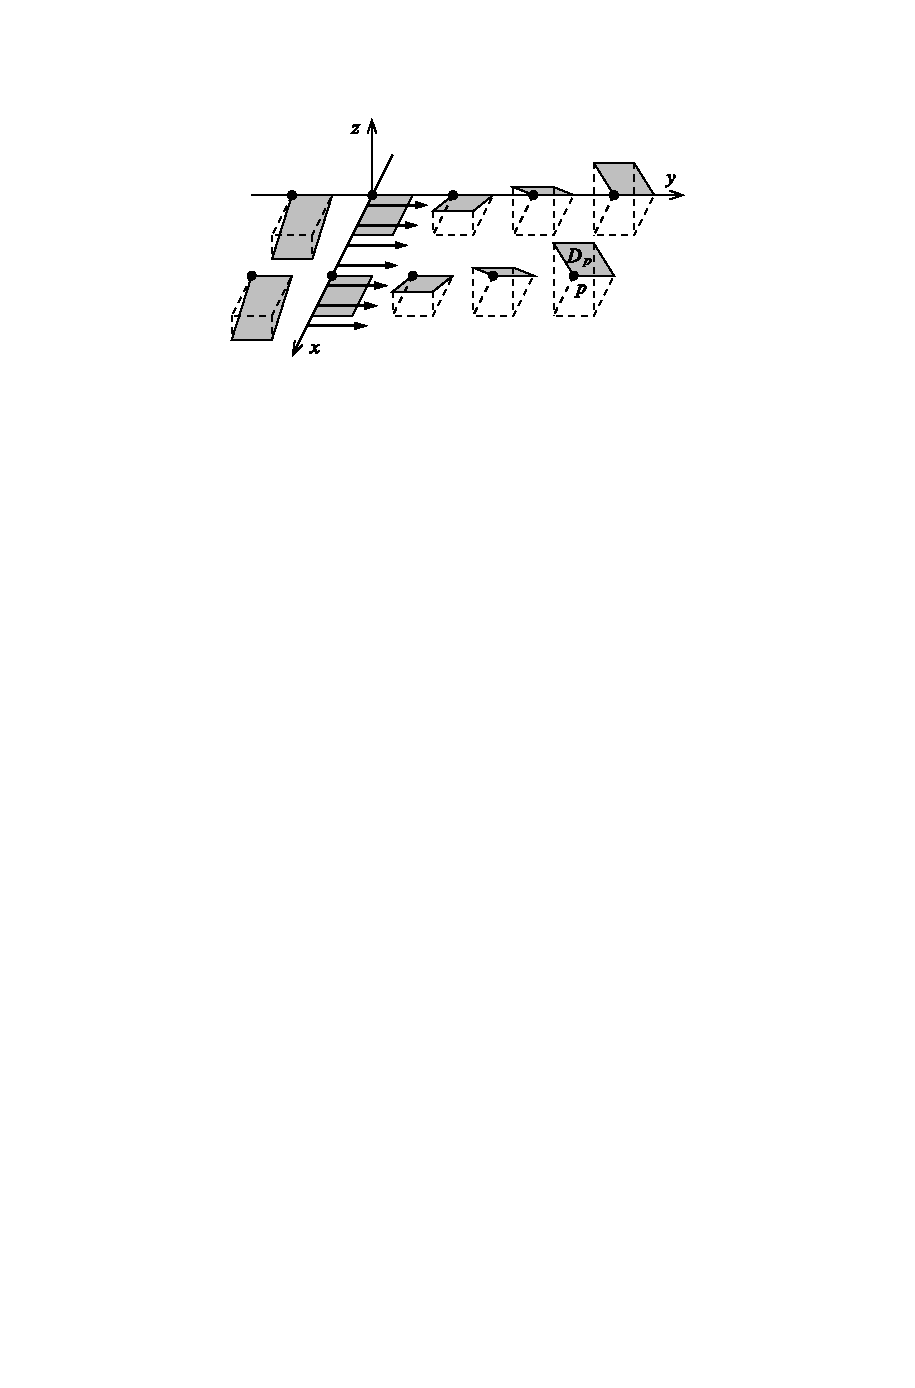
\includegraphics{pictures/distribution}
\caption{A smooth distribution with no integral manifolds.}
\end{figure}
\end{example}
The last example shows that in general, integral manifolds may fail to exist. Suppose
$D$ is a smooth distribution on $M$. We say that $D$ is \textbf{involutive} if given any pair of smooth local sections of $D$, their Lie bracket is also a local section of $D$. The next proposition shows that the involutivity condition can be expressed concisely in terms of Lie algebras.
\begin{proposition}
Let $D\sub TM$ be a smooth distribution, and let $\Gamma(D)\sub TM$ denote the space of smooth global sections of $D$. Then $D$ is involutive if and only if $\Gamma(D)$ is a Lie subalgebra of $\X(M)$.
\end{proposition}
\begin{proof}
If $D$ is involutive, the definition implies that $\Gamma(D)$ is closed under Lie brackets. Because it is also a linear subspace of $\X(M)$, 
it is a Lie subalgebra.\par
Conversely, suppose $\Gamma(D)$ is a Lie subalgebra of $\X(M)$, and let $X,Y$ be smooth local sections of $D$ over an open subset $U\sub M$. 
Given $p\in U$, let $\psi\in C^\infty(M)$ be a bump function that is identically $1$ on a neighborhood of $p$ and supported in $U$. Then $\psi X$ 
and $\psi Y$ are smooth global sections of $D$, so their Lie bracket is also a section of $D$ by hypothesis. This Lie bracket is 
$[\psi X,\psi Y]=\psi^2[X,Y]+(\psi X\psi)Y-(\psi Y\psi)X$, which is equal to $[X,Y]$ in a neighborhood of $p$. Thus, $[X,Y]\in D_p$ for each $p\in U$, 
so $D$ is involutive.
\end{proof}
A smooth distribution $D$ on $M$ is said to be \textbf{integrable} if each point of $M$ is contained in an integral manifold of $D$.
\begin{proposition}
Every integrable distribution is involutive.
\end{proposition}
\begin{proof}
Let $D\sub TM$ be an integrable distribution. Suppose $X$ and $Y$ are smooth local sections of $D$ defined on some open subset $U\sub M$. Let $p$ be any point in $U$, and let $N$ be an integral manifold of $D$ containing $p$. The fact that $X$ and $Y$ are sections of $D$ means that $X$ and $Y$ are tangent to $N$. By Corollary~\ref{Lie bracket tangent to submani}, $[X,Y]$ is also tangent to $N$, and therefore $[X,Y]_p\in D_p$. Since this is true at each $p\in U$, it follows that $D$ is involutive.
\end{proof}
Note, for example, that the distribution $D$ of Example~\ref{distribution eg}$(d)$ is not involutive, because $[X,Y]=-\partial/\partial z$, which is not a section of $D$.\par
The next lemma shows that the involutivity condition does not have to be checked
for every pair of smooth vector fields, just those of a smooth local frame in a neighborhood of each point.
\begin{lemma}[\textbf{Local Frame Criterion for Involutivity}]\label{involutivity local fram crit}
Let $D\sub TM$ be a smooth distribution. If in a neighborhood of every point of $M$ there exists a smooth local frame $V_1,\dots,V_k$ for $D$ such that $[V_i,V_j]$ is a section of $D$ for each $i,j$, then $D$ is involutive.
\end{lemma}
\begin{proof}
Suppose the hypothesis holds, and suppose $X$ and $Y$ are smooth local sections of $D$ over some open subset $U\sub M$. Given $p\in U$, choose a smooth local frame $V_1,\dots,V_k$ satisfying the hypothesis in a neighborhood of $p$, and write $X=X^iV_i$ and $Y=Y^iV_i$ in that neighborhood. Then, using $(\ref{Lie bracket two product rule})$,
\[[X,Y]=[X^iV_i,Y^jV_j]=X^iY^j[V_i,V_j]+X^i(V_iY^j)V_j-Y^j(V_jX^i)V_i.\]
It follows from the hypothesis that this last expression is a section of $D$.
\end{proof}
\subsubsection{Involutivity and differential forms}
Differential forms yield an alternative way to describe distributions and involutivity.
\begin{lemma}[\textbf{$\bm{1}$-Form Criterion for Smooth Distributions}]\label{distribution smooth crit}
Suppose $M$ is a smooth $n$-manifold and $D\sub TM$ is a distribution of rank $k$. Then $D$ is smooth if and only if each point $p\in M$ has a neighborhood $U$ on which there are smooth $1$-forms $\omega^1,\dots,\omega^{n-k}$ such that for each $q\in U$,
\begin{align}\label{defining frame-1}
D_q=\bigcap_{i=1}^{n-k}\ker\omega^i|_q.
\end{align}
\end{lemma}
\begin{proof}
First suppose that there exist such forms $\omega^1,\dots,\omega^{n-k}$ in a neighborhood of each point. The assumption $(\ref{defining frame-1})$ together with the fact that $D$ has rank $k$ implies that the forms $\omega^1,\dots,\omega^{n-k}$ are independent on $U$ for dimensional reasons. By Proposition~\ref{vector bundle local frame completion}, we can complete them to a smooth coframe $(\omega^1,\dots,\omega^n)$ on a (possibly smaller) neighborhood of each point. If $(E_1,\dots,E_n)$ is the dual frame, it is easy to check that $D$ is locally spanned by $E_{n-k+1},\dots,E_n$, so it is smooth by the local frame criterion.\par
Conversely, suppose $D$ is smooth. In a neighborhood of any $p\in M$, there are smooth vector fields $Y_1,\dots,Y_k$ spanning $D$. By Proposition~\ref{vector bundle local frame completion} again, we can complete these vector fields to a smooth local frame $Y_1,\dots,Y_n$ for $M$ in a neighborhood of $p$. With the dual coframe denoted by $(\eps^1,\dots,\eps^n)$, it follows easily that $D$ is characterized locally by
\[D_q=\bigcap_{i=1}^{n-k}\ker\eps^i|_q.\]
This completes the proof.
\end{proof}
If $D$ is a rank-$k$ distribution on a smooth $n$-manifold $M$, any $n-k$ linearly independent $1$-forms $\omega^1,\dots,\omega^{n-k}$ defined on an open subset $U\sub M$ and satisfying $(\ref{defining frame-1})$ for each $q\in U$ are called \textbf{local defining forms} for $D$. More generally, if $0\leq p\leq n$, we say that a $p$-form $\omega\in\Omega^p(M)$ \textbf{annihilates $\bm{D}$} if $\omega(X_1,\dots,X_p)=0$ whenever $X_1,\dots,X_p$ are local sections of $D$. (In the case $p=0$, only the zero function annihilates $D$.)
\begin{lemma}\label{distribution annihilate iff}
Suppose $M$ is a smooth $n$-manifold and $D$ is a smooth rank-$k$ distribution on $M$. Let $\omega^1,\dots,\omega^{n-k}$ be smooth local defining forms for $D$ over an open subset $U\sub M$. A smooth $p$-form $\eta$ defined on $U$ annihilates $D$ if and only if it can be expressed in the form
\begin{align}\label{annihilate-1}
\eta=\sum_{i=1}^{n-k}\omega^i\wedge\beta^i
\end{align}
for some smooth $(p-1)$-forms $\beta^1,\dots,\beta^{n-k}$ on $U$.
\end{lemma}
\begin{proof}
It is easy to check that any form $\eta$ that satisfies $(\ref{annihilate-1})$ in a neighborhood of each point annihilates $D$. Conversely, suppose that $\eta$ annihilates $D$ on $U$. In a neighborhood of each point we can complete the $(n-k)$-tuple $\omega^1,\dots,\omega^{n-k}$ to a smooth local coframe $\omega^1,\dots,\omega^n$ for $M$. If $(E_1,\dots,E_n)$ is the dual frame, then $D$ is locally spanned by $E_{n-k+1},\dots,E_n$. In terms of this coframe, any $\eta\in\Omega^p(M)$ can be written locally in a unique way as
\[\eta=\sum'_{I}\eta_I\,\omega^{i_1}\wedge\cdots\wedge\omega^{i_p},\]
where the coefficients $\eta_I$ are determined by $\eta_I=\eta(E_{i_1},\dots,E_{i_p})$. Thus, $\eta$ annihilates $D$ in $U$ if and only if $\eta_I=0$ whenever $n-k+1\leq i_1<\cdots<i_p\leq n$, in which case $\eta$ can be written locally as
\[\eta=\sum'_{I:i_1\leq n-k}\eta_I\,\omega^{i_1}\wedge\cdots\wedge\omega^{i_p}=\sum_{i_1=1}^{k}\omega^{i_1}\wedge\Big(\sum'_{I'}\eta_{i_1I'}\,\omega^{i_2}\wedge\cdots\wedge\omega^{i_p}\Big),\]
where we have written $I'=(i_2,\dots,i_p)$. This holds in a neighborhood of each point of $U$; patching together with a partition of unity, we obtain a similar expression on all of $U$.
\end{proof}
When expressed in terms of differential forms, the involutivity condition translates
into a statement about exterior derivatives.
\begin{theorem}[\textbf{$\bm{1}$-Form Criterion for Involutivity}]\label{involutivity 1 form crit}
Suppose $D\sub TM$ is a smooth distribution. Then $D$ is involutive if and only if the following condition is satisfied:
\begin{equation}\label{involutivity 1 form crit-1}
\parbox{\dimexpr\linewidth-6em}
{\strut
If $\eta$ is any smooth $1$-form that annihilates $D$ on an open subset $U\sub M$, then $d\eta$ also annihilates $D$ on $U$.
\strut}
\end{equation}
\end{theorem}
\begin{proof}
First, assume that $D$ is involutive, and suppose $\eta$ is a smooth $1$-form that annihilates $D$ on $U\sub M$. Then for any smooth local sections $X,Y$ of $D$, formula $(\ref{ext der 1 form})$ for $d\eta$ gives
\[d\eta(X,Y)=X(\eta(Y))-Y(\eta(X))-\eta([X,Y]).\]
The hypothesis implies that each of the terms on the right-hand side is zero on $U$.\par
Conversely, suppose $D$ satisfies $(\ref{involutivity 1 form crit-1})$, and suppose $X$ and $Y$ are smooth local
sections of $D$. If $\omega^1,\dots,\omega^{n-k}$ are smooth local defining forms for $D$, then $(\ref{ext der 1 form})$ shows that for each $1\leq i\leq n-k$,
\[\omega^i([X,Y])=X(\omega^i(Y))-Y(\omega^i(X))-d\omega^i(X,Y)=0,\]
which implies that $[X,Y]$ takes its values in $D$. Thus $D$ is involutive.
\end{proof}
Just like the Lie bracket condition for involutivity, the exterior derivative condition need only be checked for a particular set of smooth defining forms in a neighborhood of each point, as the next proposition shows.
\begin{proposition}[\textbf{Local Coframe Criterion for Involutivity}]\label{involutivity local coframe crit}
Let $D$ be a smooth distribution of rank $k$ on a smooth $n$-manifold $M$, and let $\omega^1,\dots,\omega^{n-k}$ be smooth defining forms for $D$ on an open subset $U\sub M$. The following are equivalent:
\begin{itemize}
\item[(a)] $D$ is involutive on $U$.
\item[(b)] $d\omega^1,\dots,d\omega^{n-k}$ annihilate $D$.
\item[(c)] There exist smooth $1$-forms $\{\alpha^i_j:1\leq i,j\leq n-k\}$ such that
\[d\omega^i=\sum_{j=1}^{n-k}\omega^j\wedge\alpha^i_j\for 1\leq i\leq n-k.\]
\item[$(d)$] For each $i=1,\dots,n-k$ we have
\[d\omega^i\wedge\omega^1\wedge\cdots\wedge\omega^{n-k}=0.\] 
\end{itemize}
\end{proposition}
\begin{proof}
By Theorem~\ref{involutivity 1 form crit}, if $D$ is involutive on $U$ then $d\omega^1,\dots,\omega^{n-k}$ annihilate $D$, so (a) implies (b). Now assume (b). If $\eta$ is a smooth $1$-form that annihilates $D$ on $U$, then by Proposition~\ref{distribution annihilate iff} there are smooth functions $\beta^i$ on $U$ such that
\[\eta=\sum_{i=1}^{n-k}\omega^i\wedge\beta^i.\]
Therefore
\[d\eta=\sum_{i=1}^{n-k}d\omega^i\wedge\beta^i-\sum_{i=1}^{n-k}\omega^i\wedge d\beta^i.\]
Since all $d\omega^i$'s annihilate $D$, $d\eta$ also annihilates $D$ on $U$. Thus $D$ is involutive on $U$ by Theorem~\ref{involutivity 1 form crit}. This proves $(a)\Leftrightarrow(b)$. By Lemma~\ref{distribution annihilate iff} we see (c) is equivalent to (b).\par
For $(d)$, it is clear that (c) implies $(d)$. Now assume $(d)$ holds. In a neighborhood of each point we can complete the $(n-k)$-tuple $\omega^1,\dots,\omega^{n-k}$ to a smooth local coframe $\omega^1,\dots,\omega^n$ for $M$. If $(E_1,\dots,E_n)$ is the dual frame, then $D$ is locally spanned by $E_{n-k+1},\dots,E_n$. In terms of this coframe, $d\omega^i$ can be written as
\[d\omega^i=\sum_{I}'\alpha_{I}\omega^{i_1}\wedge\omega^{i_2}.\]
The fact that $d\omega^i\wedge\omega^1\wedge\cdots\wedge\omega^{n-k}=0$ means $\alpha_{I}=0$ when $n-k+1\leq i_1<i_2\leq n$. Therefore, similar to the proof of Lemma~\ref{distribution annihilate iff}, we can write
\[d\omega^i=\sum_{i_1\leq n-k}\alpha_I\omega^{i_1}\wedge\omega^{i_2}=\sum_{i=1}^{n-k}\omega^i\wedge\Big(\sum_{i_1<i_2}\omega_{i_2}\Big).\]
By Lemma~\ref{distribution annihilate iff} this implies $d\omega^i$ annihilates $D$. Since this holds for all $i$, we get (b).
\end{proof}
With a bit more algebraic terminology, there is an elegant way to express the involutivity condition in terms of differential forms. Recall that we have defined
the graded algebra of smooth differential forms on a smooth $n$-manifold $M$ as $\Omega^*(M)=\bigoplus_{p=0}^{n}\Omega^p(M)$. An \textbf{ideal} in $\Omega^*(M)$ is a linear
subspace $\mathcal{I}\sub\Omega^*(M)$ that is closed under wedge products with arbitrary elements of $\Omega^*(M)$. Now suppose $D$ is a smooth distribution on a 
smooth $n$-manifold $M$. Let $\mathcal{I}^p(D)$ denote the space of smooth $p$-forms that annihilate $D$, and let $\mathcal{I}(D)=\bigoplus_{p=0}^{n}\mathcal{I}^p(D)$.\par
Any ideal of the form $\mathcal{I}(D)$ for some smooth distribution $D$ is sometimes called a \textbf{Pfaffian system}. An ideal $\mathcal{I}\sub\Omega^*(M)$ is said to be a \textbf{differential ideal} if $d(\mathcal{I})\sub\mathcal{I}$, that is, if $\eta\in\mathcal{I}$ implies $d\eta\in\mathcal{I}$.
\begin{proposition}[\textbf{Differential Ideal Criterion for Involutivity}]\label{involutivity differential ideal crit}
Let $M$ be a smooth manifold. A smooth distribution $D\sub TM$ is involutive if and only if $\mathcal{I}(D)$ is a differential ideal in $\Omega^*(M)$.
\end{proposition}
\begin{proof}
One direction is given by Theorem~\ref{involutivity 1 form crit}, the other is proved by Lemma~\ref{distribution annihilate iff}.
\end{proof}
\subsection{The Frobenius theorem}
Given a rank-$k$ distribution $D\sub TM$, let us say that a smooth coordinate chart $(U,\varphi)$ on $M$ is \textbf{flat} for $D$ if $\varphi(U)$ is a cube in $\R^n$, and at points of $U$, $D$ is spanned by the first $k$ coordinate vector fields $\partial/\partial x^1,\dots,\partial/\partial x^k$. In any such chart, each slice of the form $\{x^{k+1}=c^{k+1},\dots,x^n=c^n\}$ for constants $c^{k+1},\dots,c^n$ is an integral manifold of $D$. This is the nicest possible local situation for integral manifolds. We say that a distribution $D\sub TM$ is \textbf{completely integrable} if there exists a flat chart for $D$ in a neighborhood of each point of $M$. Obviously, every completely integrable distribution is integrable and therefore involutive. In summary,
\[\text{completely integrable}\Longrightarrow\text{integrable}\Longrightarrow\text{involutive}.\]
The next theorem is the main result of this section, and indeed one of the central theorems in smooth manifold theory. It says that the implications above are actually equivalences:
\[\text{completely integrable}\iff\text{integrable}\iff\text{involutive}.\]
\begin{figure}[htbp]
\centering
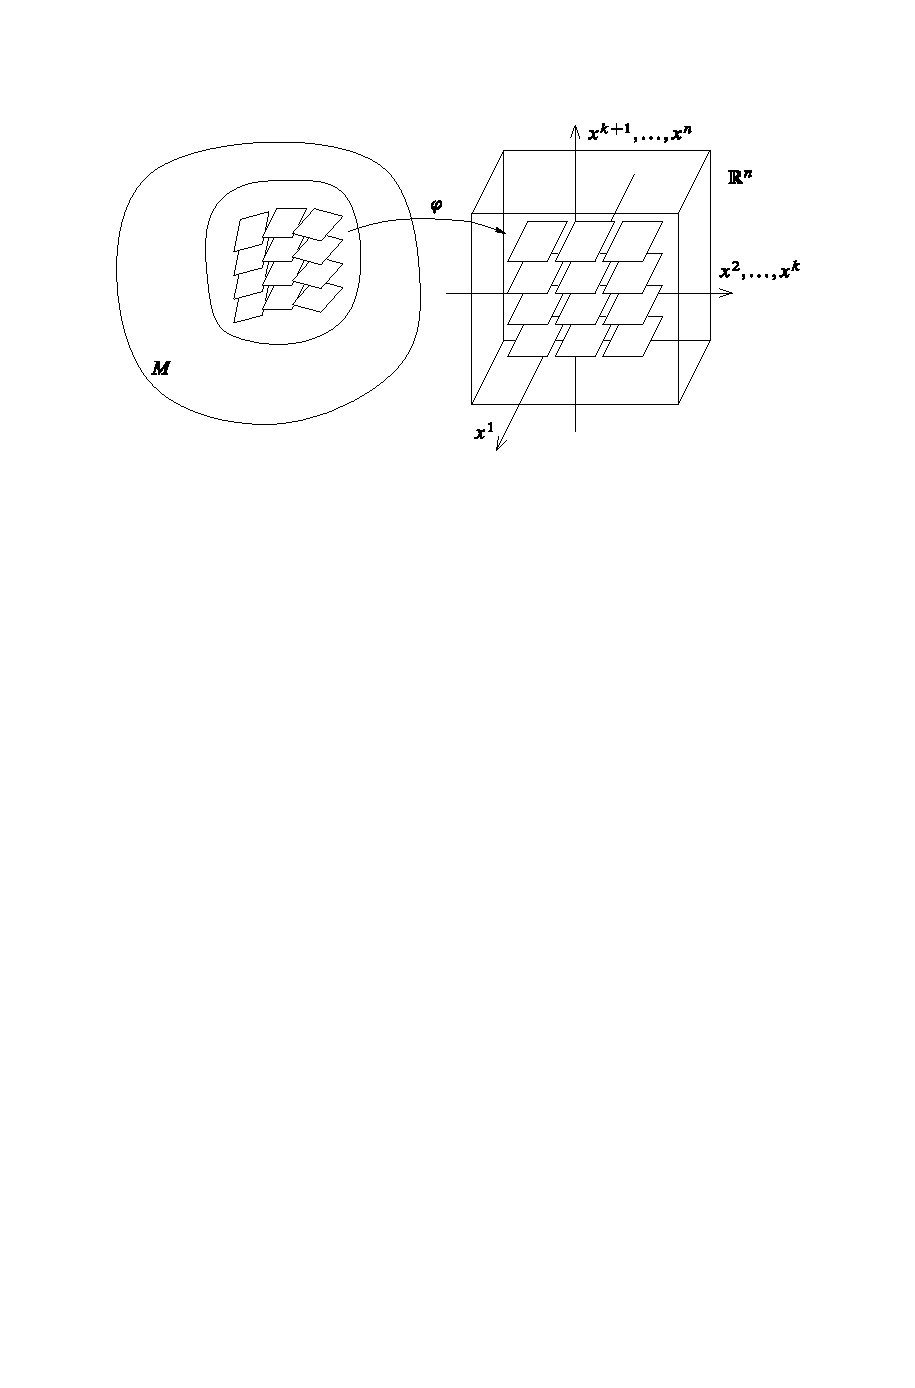
\includegraphics{pictures/flat-chart}
\caption{A flat chart for a distribution.}
\end{figure}
\begin{theorem}[\textbf{Frobenius}]
Every involutive distribution is completely integrable.
\end{theorem}
\begin{proof}
The canonical form theorem for commuting vector fields (Theorem~\ref{flow commute canonical form}) implies that any distribution locally spanned by independent smooth commuting vector fields is completely integrable, because the coordinate chart whose existence is guaranteed by that theorem is flat (after shrinking the domain if necessary so the image is a cube). Thus, it suffices to show that every involutive distribution is locally spanned by independent smooth commuting vector fields.\par
Let $D$ be an involutive distribution of rank $k$ on an $n$-dimensional manifold $M$, and let $p\in M$. Since complete integrability is a local question, by passing to a smooth coordinate neighborhood of $p$, we may replace $M$ by an open subset $U\sub\R^n$, and choose a smooth local frame $X_1,\dots,X_k$ for $D$. By reordering the coordinates if necessary, we may assume that $D_p$ is complementary to the subspace of $T_p\R^n$ spanned by $\partial/\partial x^{k+1}|_p,\dots,\partial/\partial x^{n}|_p$.\par 
Let $\pi:\R^n\to\R^k$ be the projection onto the first $k$ coordinates. This induces a smooth bundle homomorphism $d\pi:T\R^n\to T\R^k$, which can be written
\[d\pi\Big(\sum_{i=1}^{n}v^i\frac{\partial}{\partial x^i}\Big|_{q}\Big)=\sum_{i=1}^{k}v^i\frac{\partial}{\partial x^i}\Big|_{\pi(q)}.\]
Because $d\pi|_D$ is the composition of the inclusion $D\hookrightarrow U$ followed by $d\pi$, it is a smooth bundle homomorphism. Thus, the matrix entries of $d\pi|_{D_q}$ with respect to the frames $(X_i|_q)$ and $(\partial/\partial x^j|_{\pi(q)})$ are smooth functions of $q$.\par
By our choice of coordinates, $D_p\sub T_p\R^n$ is complementary to the kernel of $d\pi_p$, so the restriction of $d\pi_p$ to $D_p$ is bijective. By continuity, therefore, the same is true of $d\pi_{D_q}$ for $q$ in a neighborhood of $p$, and the matrix entries of $(d\pi|_{D_q})^{-1}:T_{\pi(q)}\R^k\to D_q$ are also smooth functions of $q$. Define a new smooth local frame $V_1,\dots,V_k$ for $D$ in a neighborhood of $p$ by 
\[V_i|_q=(d\pi|_{D_q})^{-1}\frac{\partial}{\partial x^i}\Big|_{\pi(q)}.\]
The theorem will be proved if we can show that $[V_i,V_j]=0$ for all $i,j$.\par
First observe that $V_i$ and $\partial/\partial x^i$ are $\pi$-related, because
\[\frac{\partial}{\partial x^i}\Big|_{\pi(q)}=(d\pi|_{D_q})V_i|_q=d\pi_q(V_i|_q).\]
Therefore, by the naturality of Lie brackets,
\[d\pi_q([V_i,V_j]_q)=\Big[\frac{\partial}{\partial x^i},\frac{\partial}{\partial x^j}\Big]_{\pi(q)}=0.\]
Since involutivity of $D$ implies that $[V_i,V_j]$ takes its values in $D$, and $d\pi$ is injective on each fiber of $D$, this implies that $[V_i,V_j]=0$ for each $q$, thus completing the proof.
\end{proof}
For later use in our treatment of overdetermined partial differential equations, we note the following easy corollary to the proof.
\begin{corollary}\label{distribution complementary submani is slice}
Suppose $M$ is a smooth manifold, $D$ is an involutive rank-$k$ distribution on $M$, and $S\sub M$ is a codimension-$k$ embedded submanifold. If $p\in S$ is a point such that $T_pS$ is complementary to $D_p$, then there is a flat chart $(U,(s^i))$ for $D$ centered at $p$ in which $S\cap U$ is the slice $s^1=\cdots=s^k=0$.
\end{corollary}
\begin{proof}
The proof of the theorem showed that locally $D$ is spanned by $k$ commuting vector fields, and then the corollary follows from Theorem~\ref{flow commute canonical form}.
\end{proof}
As is often the case, embedded in the proof of the Frobenius theorem is a technique for finding integral manifolds. The idea is to use a coordinate projection to find commuting vector fields spanning the same distribution, and then use the technique of Example~\ref{commute vector field eg} to find a flat chart. Here is an example.
\begin{example}
Let $D\sub T\R^3$ be the distribution spanned by the vector fields
\begin{flalign*}
&X=x\frac{\partial}{\partial x}+\frac{\partial}{\partial y}+x(y+1)\frac{\partial}{\partial z},\\
&Y=\frac{\partial}{\partial x}+y\frac{\partial}{\partial z}
\end{flalign*}
We have
\[[X,Y]=-\frac{\partial}{\partial x}-y\frac{\partial}{\partial z}=-Y,\]
so $D$ is involutive. Let us try to find a flat chart in a neighborhood of the origin. Since $D$ is complementary to the span of $\partial/\partial z$, the coordinate projection $\pi:\R^3\to\R^2$ given by $\pi(x,y,z)=(x,y)$ induces an isomorphism $d\pi|_{D_{(x,y,z)}}:D_{(x,y,z)}\to T_{(x,y)}\R^2$ for each $(x,y,z)$. The proof of the Frobenius theorem shows that if we can find smooth local sections $V,W$ of $D$ that are $\pi$-related to $\partial/\partial x$ and $\partial/\partial y$, respectively, they will be commuting vector fields spanning $D$. It is easy to check that $V,W$ have this property if and only if they take their values in $D$ and are of the form
\begin{flalign*}
&V=\frac{\partial}{\partial x}+u(x,y,z)\frac{\partial}{\partial z},\\
&W=\frac{\partial}{\partial y}+v(x,y,z)\frac{\partial}{\partial z},
\end{flalign*}
for some smooth real-valued functions $u,v$. A bit of linear algebra shows that the vector fields
\begin{flalign*}
&V=Y=\frac{\partial}{\partial x}+y\frac{\partial}{\partial z},\\
&W=X-xY=\frac{\partial}{\partial y}+x\frac{\partial}{\partial z},
\end{flalign*}
do the trick. Sparing the details, we find that the flow of $V$ is
\[\alpha_t(x,y,z)=(x+t,y,z+ty),\]
and that of $W$ is
\[\beta_t(x,y,z)=(x,y+t,z+tx).\]
Thus, by the procedure of Example~\ref{commute vector field eg}, we can define the inverse $\varPhi$ of our coordinate map by starting on the $z$-axis and flowing out along these two flows in succession:
\[\varPhi(u,v,w)=\alpha_u\circ\beta_v(0,0,w)=\alpha_u(0,0,w)=(u,v,w+uv).\]
The flat coordinates we seek are given by inverting the map $(x,y,z)=\varPhi(u,v,w)=(u,v,w+uv)$, to yield
\[(u,v,w)=\varPhi^{-1}(x,y,z)=(x,y,z-xy).\]
It follows that the integral manifolds of $D$ are the level sets of $w(x,y,z)=z-xy$.
\end{example}
The next proposition is one of the most important consequences of the Frobenius
theorem.
\begin{proposition}[\textbf{Local Structure of Integral Manifolds}]\label{integral mani local struct}
Let $D$ be an involutive distribution of rank $k$ on a smooth manifold $M$, and let $(U,(x^i))$ be a flat chart for $D$. If $H$ is any integral manifold of $D$, then $H\cap U$ is a union of countably many disjoint open subsets of parallel $k$-dimensional slices of $U$, each of which is open in $H$ and embedded in $M$.
\end{proposition}
\begin{figure}[htbp]
\centering
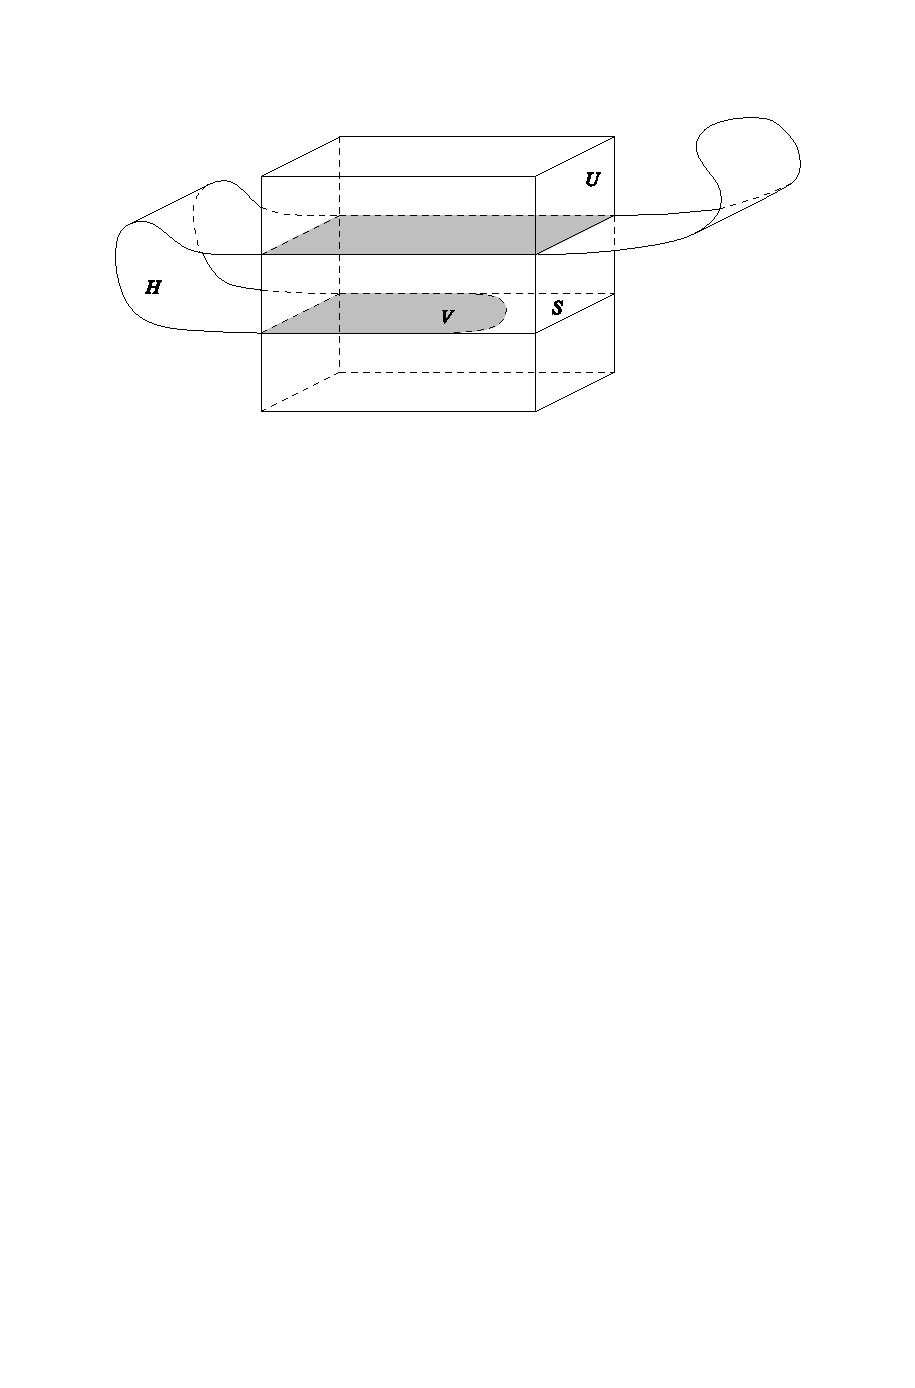
\includegraphics{pictures/local-struct}
\caption{The local structure of an integral manifold.}
\end{figure}
\begin{proof}
Let $H$ be an integral manifold of $D$. Because the inclusion map $\iota:H\hookrightarrow M$ is continuous, $H\cap U=\iota^{-1}(U)$ is open in $H$, and thus consists of a countable disjoint union of connected components, each of which is open in $H$.\par
Let $V$ be any component of $H\cap U$. We show first that $V$ is contained in a single slice. Since $dx^{k+1},\dots,dx^n$ are local defining forms for $D$, it follows that the pullbacks of these $1$-forms to $V$ are identically zero. Because $V$ is connected, this implies that $x^{k+1},\dots,x^n$ are all constant on $V$, so $V$ lies in a single slice $S$.\par
Because $S$ is embedded in $M$, the inclusion map $V\hookrightarrow M$ is also smooth as a map into $S$ by Corollary~\ref{resrtict codomain to embedd}. The inclusion $V\hookrightarrow S$ is thus an injective smooth immersion between manifolds of the same dimension, and therefore a local diffeomorphism, an open map, and a homeomorphism onto an open subset of $S$. The inclusion map $V\hookrightarrow M$ is a composition of the smooth embeddings $V\hookrightarrow S\hookrightarrow M$, so it is a smooth embedding.
\end{proof}
The preceding proposition implies the following important result about integral
manifolds, which we will use in our study of Lie subgroups at the end of this section. Recall that a smooth submanifold $H\sub M$ is said to be weakly embedded in $M$ if every smooth map $F:N\to M$ whose image lies in $H$ is smooth as a map from $N$ to $H$.
\begin{theorem}\label{integral mani weak embedd}
Every integral manifold of an involutive distribution is weakly embedded.
\end{theorem}
\begin{proof}
Let $M$ be a smooth $n$-manifold, let $H\sub M$ be an integral manifold of an involutive rank-$k$ distribution $D$ on $M$, and suppose $F:N\to M$ is a smooth map such that $F(N)\sub H$. Let $p\in N$ be arbitrary, and set $q=F(p)\in H$. Let $(y^1,\dots,y^n)$ be flat coordinates for $D$ on a neighborhood $U$ of $q$, and let $(x^i)$ be smooth coordinates for $N$ on a connected neighborhood $B$ of $p$ such that $F(B)\sub U$. With the coordinate representation of $F$ written as
\[(y^1,\dots,y^n)=(F^1(x),\dots,F^n(x)).\]
The fact that $F(N)\sub H\cap U$ means that the coordinate functions $F^{k+1}(x),\dots,F^n(x)$ take on only countably many values. Because $B$ is connected, the intermediate value theorem implies that these coordinate functions are constant, and thus $F(B)$ lies in a single slice $S\sub U$. Because $S\cap H$ is an open subset of $H$ that is embedded in $M$, it follows that $F|_B$ is smooth from $B$ into $S\cap H$, and thus by composition, $F|_B:D\hookrightarrow(S\cap H)\hookrightarrow H$ is smooth into $H$.
\end{proof}
\subsection{Foliations}
When we put together all of the maximal integral manifolds of an involutive rank-$k$ distribution on a smooth manifold $M$, we obtain a partition of $M$ into $k$-dimensional submanifolds that fit together locally like the slices in a flat chart.\par 
To express more precisely what we mean by fitting together, we need to extend our notion of a flat chart slightly. Let $M$ be a smooth $n$-manifold, and let $\mathcal{F}$ be any collection of $k$-dimensional submanifolds of $M$. A smooth chart $(U,\varphi)$ for $M$ is said to be \textbf{flat for $\mathcal{F}$} if $\varphi(U)$ is a cube in $\R^n$, and each submanifold in $\mathcal{F}$ intersects $U$ in either the empty set or a countable union of $k$-dimensional slices of the form $\{x^{k+1}=c^{k+1},\dots,x^n=c^n\}$. We define a \textbf{foliation of dimension $\bm{k}$ on $\bm{M}$} to be a collection $\mathcal{F}$ of disjoint, connected, nonempty, immersed $k$-dimensional submanifolds of $M$ (called the \textbf{leaves of the foliation}), whose union is $M$, and such that in a neighborhood of each point $p\in M$ there exists a flat chart for $\mathcal{F}$.
\begin{example}[\textbf{Foliations}]
\mbox{}
\begin{itemize}
\item[(a)] The collection of all $k$-dimensional affine subspaces of $\R^n$ parallel to $\R^k\times\{0\}$ is a $k$-dimensional foliation of $\R^n$.
\item[(b)] The collection of open rays of the form $\{\lambda x:\lambda>0\}$ as $x$ ranges over $\R^n-\{0\}$ is a $1$-dimensional foliation of $\R^n-\{0\}$.
\item[(c)] The collection of all spheres centered at $0$ is an $(n-1)$-dimensional foliation of $\R^n-\{0\}$.
\begin{figure}[htbp]
\centering
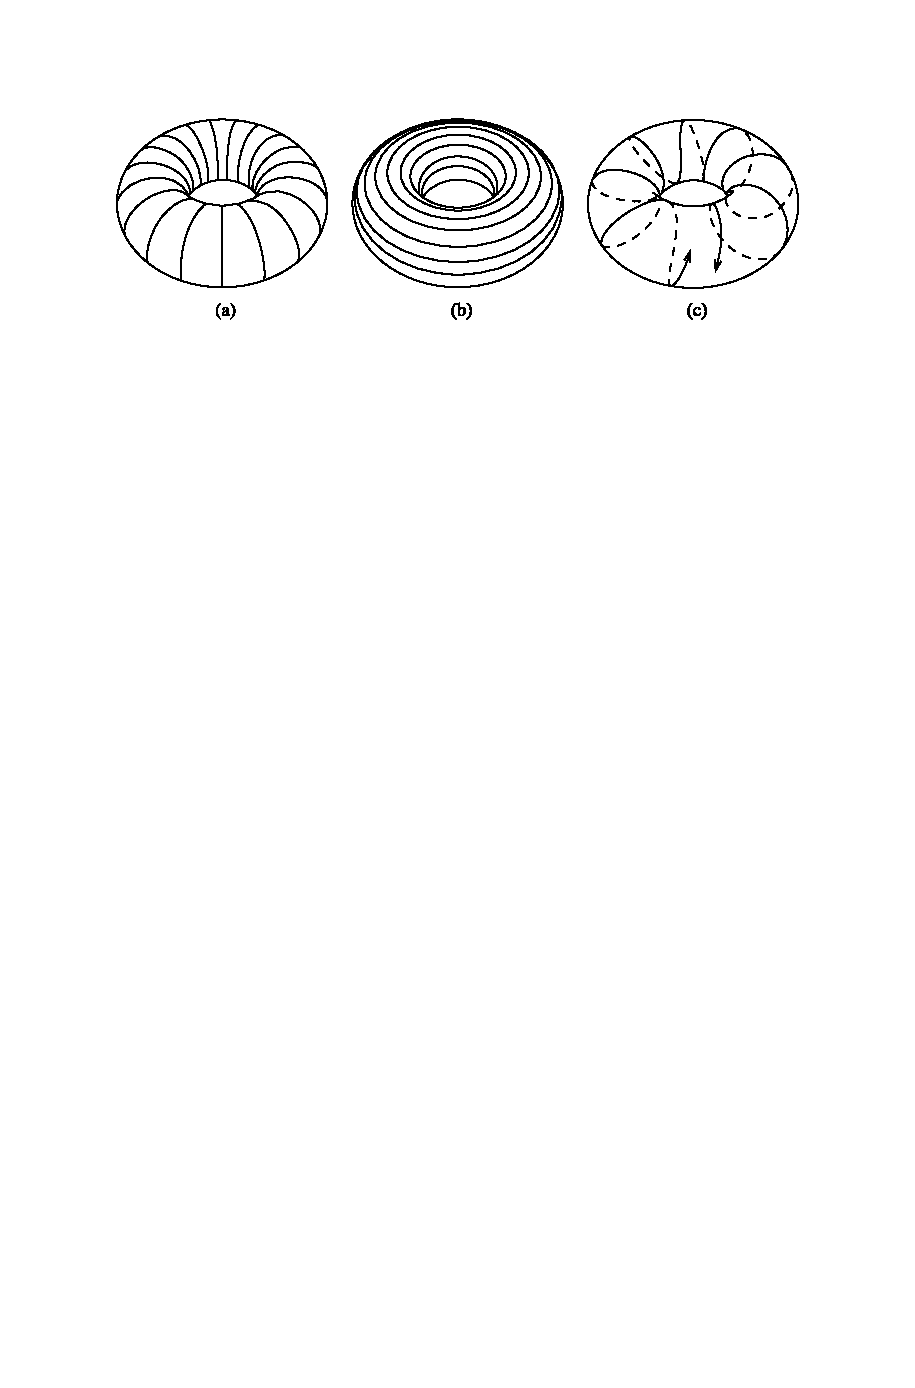
\includegraphics{pictures/foliation-of-torus}
\caption{Foliations of the torus.}
\end{figure} 
\item[$(d)$] If $M$ and $N$ are connected smooth manifolds, the collection of subsets of the form $M\times\{q\}$ as $q$ ranges over points in $N$ forms a foliation of $M\times N$, each of whose leaves is diffeomorphic to $M$. For example, the collection of all circles of the form $S^1\times\{q\}\sub T^2$ for $q\in S^1$ yields a foliation of the torus $T^2$. A different foliation of $T^2$ is given by the collection of circles of the form $\{p\}\times S^1$.
\item[$(e)$] If $\alpha$ is a fixed real number, the images of all curves of the form
\[\gamma_\theta(t)=(e^{it},e^{i(\alpha t+\theta)})\]
as $\theta$ ranges over $\R$ form a $1$-dimensional foliation of the torus. If $\alpha$ is rational, each leaf is an embedded circle; whereas if $\alpha$ is irrational, each leaf is dense.
\item[(f)] The collection of connected components of the curves in the $(y,z)$-plane defined by the following equations is a foliation of $\R^2$:
\begin{flalign*}
&z=\sec y+c,\ c\in\R;\\
&y=(k+\frac{1}{2})\pi,\ k\in\Z.
\end{flalign*}
\item[(g)] If we revolve the curves of the previous example around the $z$-axis, we obtain a $2$-dimensional foliation of $\R^3$ in which some of the leaves are diffeomorphic to disks and some are diffeomorphic to cylinders.
\end{itemize}
\end{example}
\begin{figure}[htbp]
\centering
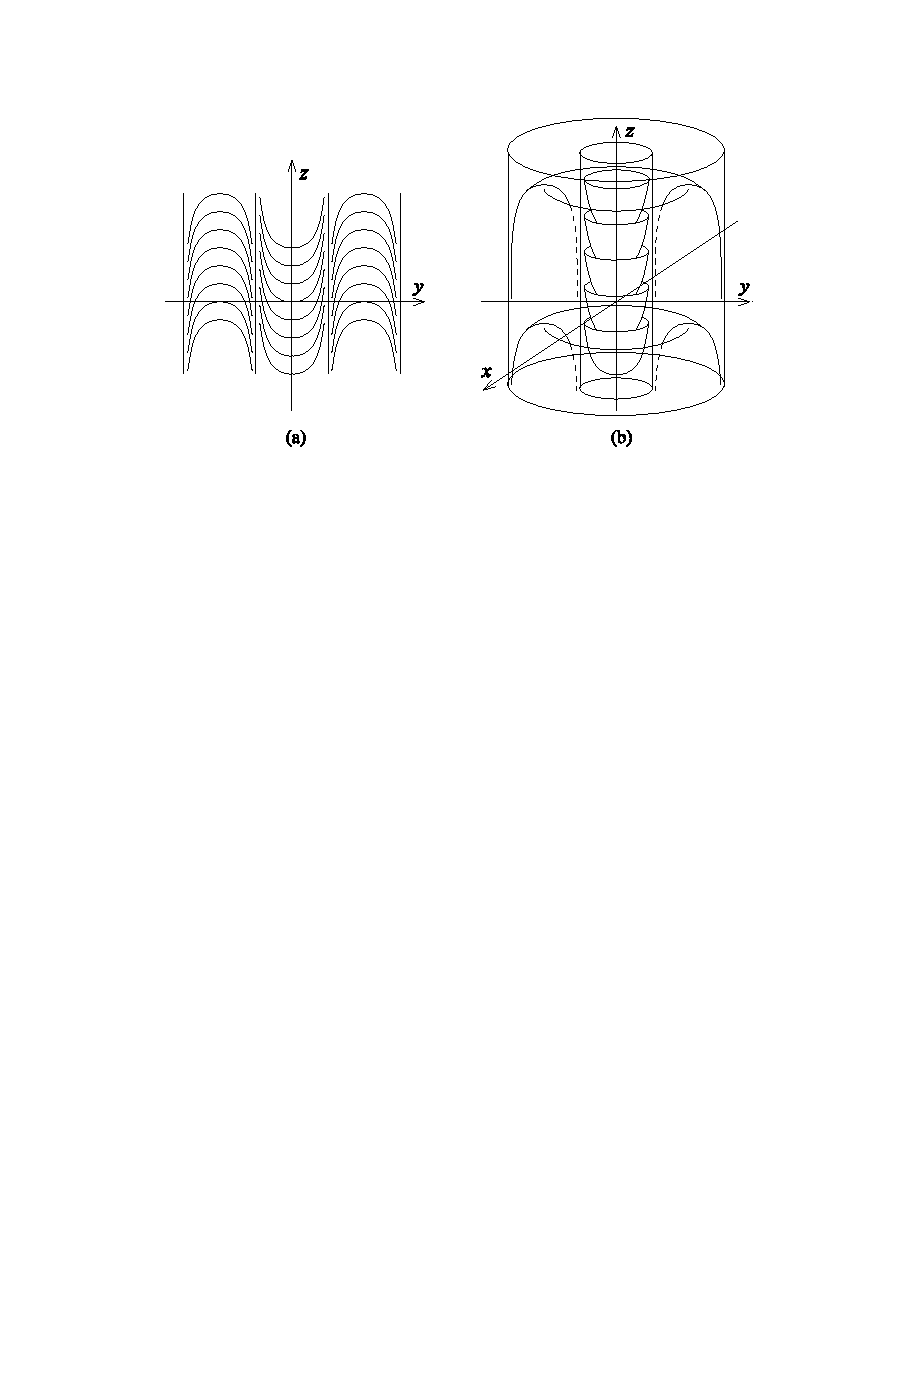
\includegraphics{pictures/foliation}
\caption{Foliations of $\R^2$ and $\R^3$.}
\end{figure}
The main fact about foliations is that they are in one-to-one correspondence with
involutive distributions. One direction, expressed in the next proposition, is an easy consequence of the definition.
\begin{proposition}
Let $\mathcal{F}$ be a foliation on a smooth manifold $M$. The collection of tangent spaces to the leaves of $\mathcal{F}$ forms an involutive distribution on $M$.
\end{proposition}
The Frobenius theorem allows us to conclude the following converse, which is much more profound. By the way, it is worth noting that this result is one of the two primary reasons why the notion of immersed submanifold has been defined.
\begin{theorem}[\textbf{Global Frobenius Theorem}]
Let $D$ be an involutive distribution on a smooth manifold $M$. The collection of all maximal connected integral manifolds of $D$ forms a foliation of $M$.
\end{theorem}
The theorem will be an easy consequence of the following lemma.
\begin{lemma}
Suppose $D\sub TM$ is an involutive distribution, and let $\{N_\alpha\}_{\alpha\in A}$ be any collection of connected integral manifolds of $D$ with a point in common. Then $N=\bigcup_{\alpha\in A}N_\alpha$ has a unique smooth manifold structure making it into a connected integral manifold of $D$.
\end{lemma}
\begin{proof}
If we can construct a topology and smooth manifold structure making $N$ into an integral manifold of $D$, then Theorem~\ref{unique smooth weak embedd} shows that the topology and smooth structure are uniquely determined, because integral manifolds are weakly embedded.\par
To construct the topology, first we need to show that $N_\alpha\cap N_\beta$ is open in $N_\alpha$ and in $N_\beta$ for each $\alpha,\beta\in A$. Let $q\in N_\alpha\cap N_\beta$ be arbitrary, and choose a flat chart for $D$ on a neighborhood $W$ of $q$. Let $V_\alpha,V_\beta$ denote the components of $N_\alpha\cap W$ and $N_\beta\cap W$, respectively, containing $q$. By Proposition~\ref{integral mani local struct}, $V_\alpha$ and $V_\beta$ are open subsets of single slices with the subspace topology, and since both contain $q$, they both must lie in the same slice $S$. Thus $V_\alpha\cap V_\beta$ is open in $S$ and also in both $N_\alpha$ and $N_\beta$, so $q$ has a neighborhood in $N_\alpha$ and a neighborhood in $N_\beta$ contained in $N_\alpha\cap N_\beta$.
\begin{figure}[htbp]
\centering
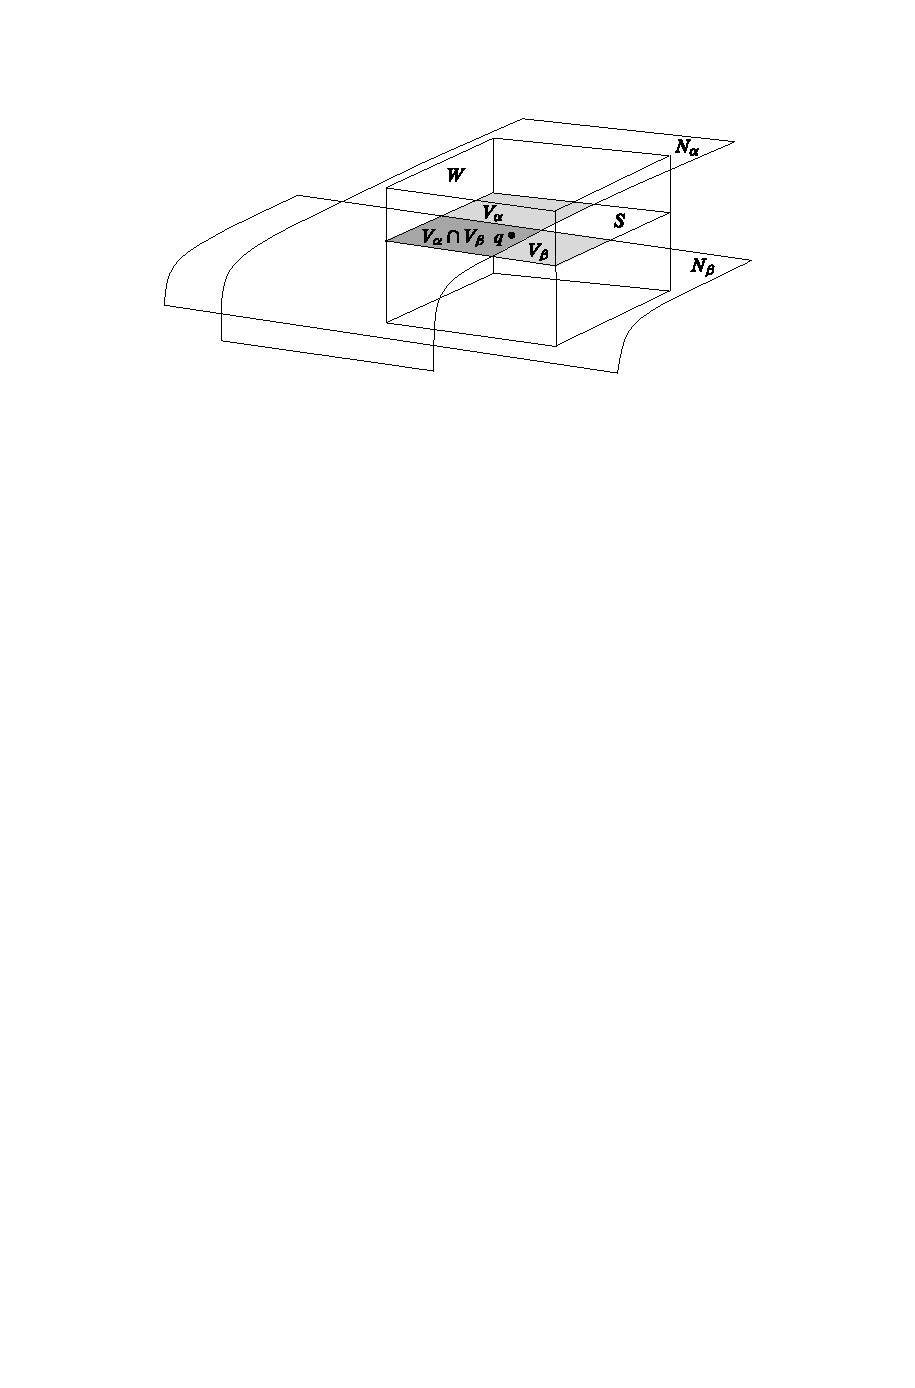
\includegraphics{pictures/union-integral-submani}
\caption{A union of integral manifolds.}
\end{figure}

Define a topology on $N$ by declaring a subset $U\sub N$ to be open if and only if $U\cap N_\alpha$ is open in $N_\alpha$ for each $N_\alpha$. Using the result of the previous paragraph, it is easy to check that this is a topology and that each $N_\alpha$ is an open subspace of $N$. With this topology, $N$ is locally Euclidean of dimension $k$, because each $q\in N$ has a coordinate neighborhood $V$ in some $N_\alpha$, and $V$ is an open subset of $N$ because $N_\alpha$ is open in $N$. Moreover, the inclusion map $N\hookrightarrow M$ is continuous: for any open subset $U\sub M$, $U\cap N$ is open in $N$ because $U\cap N_\alpha$ is open in $N_\alpha$ for each $\alpha$.\par
To see that $N$ is Hausdorff, let $q_1,q_2$ be distinct points of $N$. There are disjoint open subsets $U_1,U_2\sub M$ containing $q_1$ and $q_2$, respectively, and because inclusion $N\hookrightarrow M$ is continuous, $N\cap U_1$ and $N\cap U_2$ are disjoint open subsets of $N$ containing $q_1$ and $q_2$.\par
Next we show that $N$ is second-countable. We can cover $M$ with countably many flat charts for $D$, say $\{W_i\}$. It suffices to show that $N\cap W_i$ is contained in a countable union of slices for each $i$, because any open subset of a single slice is second countable, and thus $N$ can be expressed as a union of countably many subsets, each of which is second-countable and open in $N$.\par
Let $p_0$ be a point contained in $N_\alpha$ for every $\alpha$. Let us say that a slice $S$ of some $W_k$ is \textbf{accessible from $\bm{p_0}$} if there is a finite sequence of indices $i_1,\dots,i_m$ and for each $i_j$ a slice $S_{i_j}\sub W_{i_j}$ with the properties that $p\in S_{i_1}$, $S_{i_m}=S$, and $S_{i_j}\cap S_{i_j+1}\neq\emp$ for each $j=1,\dots,m-1$.
\begin{figure}[htbp]
\centering
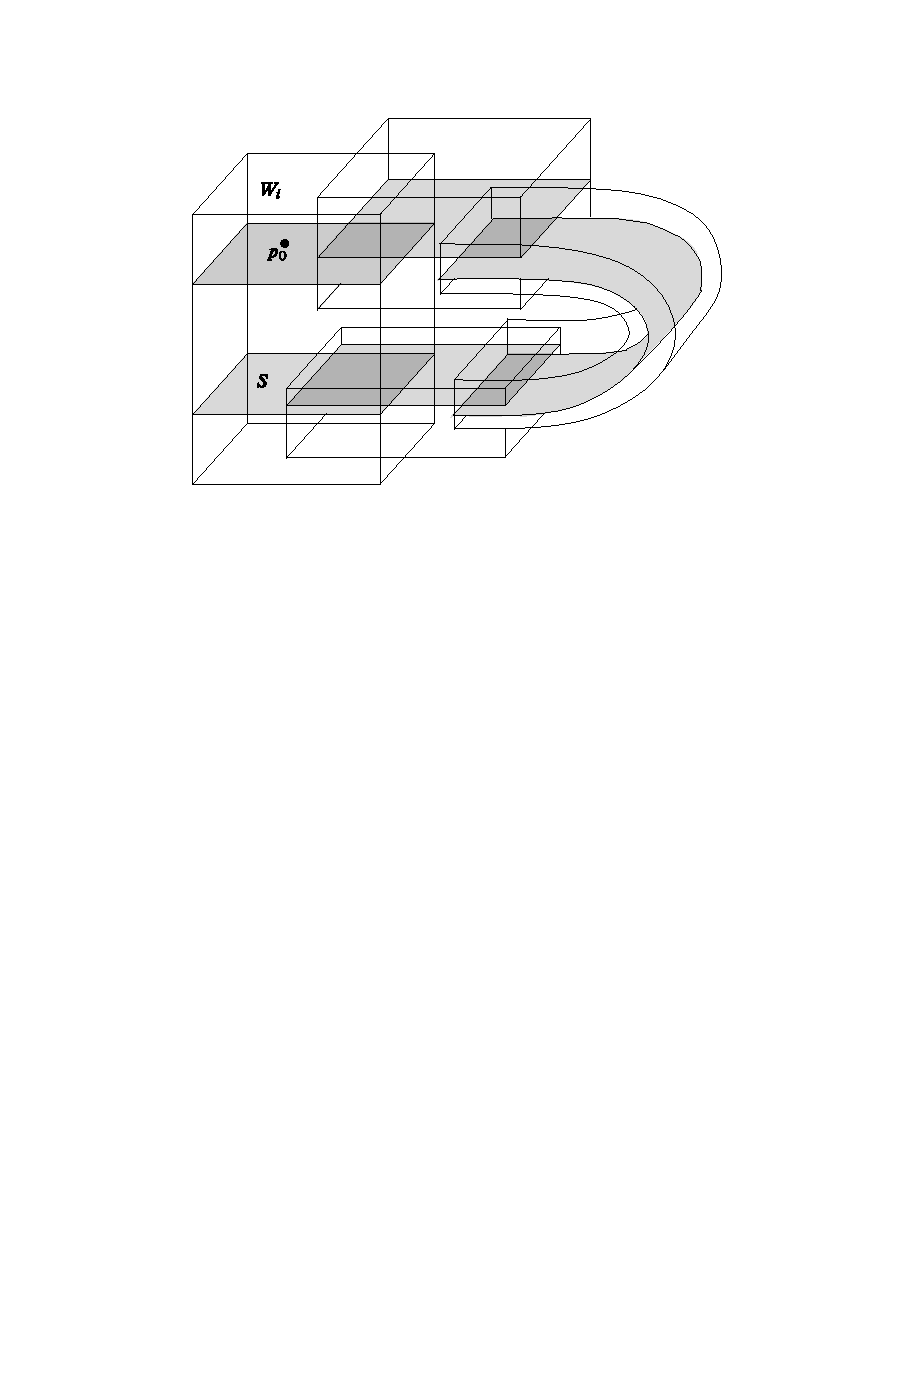
\includegraphics{pictures/slice-accessible}
\caption{A slice $S$ accessible from $p_0$}
\end{figure}

Let $W_k$ be one of our countable collection of flat charts, and suppose $S\sub W_k$ is a slice that contains a point $q\in N$. Then $q$ is contained in one of the integral manifolds $N_\alpha$. Because $p_0$ is also in $N_\alpha$, there is a continuous path $\gamma:[0,1]\to N_\alpha$ connecting $p_0$ and $q$. Since $\gamma([0,1])$ is compact, there exist finitely many numbers $0=t_0<t_1<\cdots<t_m=1$ such that for each $j=1,\dots,m$, the set $\gamma([t_{j-1},t_j])$ is contained in one of the flat charts $W_{i_j}$. Since $\gamma([t_{j-1},t_j])$ is connected, it is contained in a single component of $W_{i_j}\cap N_\alpha$ and therefore in a single slice $S_{i_j}\sub W_{i_j}$. For each $j=1,\dots,m-1$, the slices $S_{i_j}$ and $S_{i_{j+1}}$ have the point $\gamma(t_j)$ in common, so it follows that the slice $S$ is accessible from $p_0$.\par
This shows that every slice of some $W_k$ containing a point of $N$ is accessible from $p_0$, and therefore every slice intersecting $N$ must be accessible from $p_0$. To complete the proof of second-countability, we just note that each $S_{i_j}$ is itself an integral manifold, and therefore it meets at most countably many slices of $W_{i_{j+1}}$ by Proposition~\ref{integral mani local struct}; thus, there are only countably many slices accessible from $p_0$. Therefore, $N$ is a topological manifold of dimension $k$. It is connected because it is a union of connected subspaces with a point in common.\par
To construct a smooth structure on $N$, we define an atlas consisting of all charts of the form $(S\cap N,\psi)$, where $S$ is a single slice of some flat chart, and $\psi:S\to\R^k$ is the map whose coordinate representation in the flat chart is projection onto the first $k$ coordinates: $(x^1,\dots,x^k,x^{k+1},\dots,x^n)\mapsto(x^1,\dots,x^k)$. Because any slice is an embedded submanifold, its smooth structure is uniquely determined, and thus whenever two such slices $S_1$ and $S_2$ overlap the transition map $\psi_2\circ\psi_1^{-1}$ is smooth. With respect to this smooth structure, the inclusion map $N\hookrightarrow M$ is a smooth immersion (because it is a smooth embedding on each slice), and the tangent space to $N$ at each point $q\in N$ is equal to $D_q$ (because this is true for slices).
\end{proof}
\begin{proof}[Proof of the global Frobenius theorem]
For each $p\in M$, let $L_p$ be the union of all connected integral manifolds of $D$ containing $p$. By the preceding lemma, $L_p$ is a connected integral manifold of $D$ containing $p$, and it is clearly maximal. If any two such maximal integral manifolds $L_p$ and $L_{p'}$ intersect, their union $L_p\cup L_{p'}$ is an integral manifold containing both $p$ and $p'$, so by maximality $L_p=L_{p'}$. Thus, the various maximal connected integral manifolds are either disjoint or identical.\par
If $(U,\varphi)$ is any flat chart for $D$, then $L_p\cap U$ is a countable union of open subsets of slices by Proposition~\ref{integral mani local struct}. For any such slice $S$, if $L_p\cap S$ is neither empty nor all of $S$, then $L_p\cup S$ is a connected integral manifold properly containing $L_p$, which contradicts the maximality of $L_p$. Therefore, $L_p\cap U$ is precisely a countable union of slices, so the collection $\{L_p:p\in M\}$ is the desired foliation.
\end{proof}
Suppose $M$ is a smooth manifold and $\varPhi:M\to M$ is a diffeomorphism. A distribution 
$D$ on $M$ is said to be \textbf{$\varPhi$-invariant} if $d\varPhi(D)=D$ or more precisely if for 
each $x\in M$, $d\varPhi_x(D_x)=D_{\varPhi(x)}$. Similarly, a foliation $\mathcal{F}$ on 
$M$ is said to be \textbf{$\varPhi$-invariant} if for each leaf $L$ of $\mathcal{F}$, the 
submanifold $\varPhi(L)$ is also a leaf of $\mathcal{F}$.
\begin{proposition}\label{distribution invariant}
Let $M$ be a smooth manifold and $\varPhi:M\to M$ be a diffeomorphism. Suppose $D$ is an 
involutive distribution on $M$ and $\mathcal{F}$ is the foliation it determines. Then $D$ 
is $\varPhi$-invariant if and only if $\mathcal{F}$ is $\varPhi$-invariant.
\end{proposition}
\begin{proof}
Since the tangent space of a point on the leaf of the foliation is the fiber of the distribution, if 
$\mathcal{F}$ is $\varPhi$-invariant, then $D$ is also $\varPhi$-invariant. Conversely, if 
$D$ is $\varPhi$-invariant, then for any point $p\in M$, we have $d\varPhi_p(D)=D_{\varPhi(p)}$. Let $L$ be a leaf of $\mathcal{F}$, then $\varPhi(L)$ is also an integral manifold. By definition, this implies $\mathcal{F}$ is $\varPhi$-invariant.
\end{proof}
\subsection{Overdetermined systems of partial differential equations}
The partial differential equations we considered in Section~\ref{flow section} were all single equations for one unknown function. In some applications, it is necessary to consider systems of PDEs that are \textbf{overdetermined}, which means that there are more equations than unknown functions. In general, overdetermined systems have solutions only if they satisfy certain compatibility conditions. For some first-order systems, the compatibility condition can be interpreted as a statement about involutivity of a distribution, and the Frobenius theorem can be used to prove local existence and uniqueness of solutions.\par
First, we consider certain linear systems. Suppose $W$ is an open subset of $\R^n$ and $m$ is a positive integer less than or equal to $n$. Consider the following system of
\begin{equation}\label{overdetermined linear PDE}
\left\{\begin{aligned}
a^1_1(x)\frac{\partial u}{\partial x^1}(x)+\cdots+a_1^n(x)\frac{\partial u}{\partial x^n}(x)&=f_1(x),\\
&\ \ \vdots\\
a^1_m(x)\frac{\partial u}{\partial x^1}(x)+\cdots+a_m^n(x)\frac{\partial u}{\partial x^n}(x)&=f_m(x)
\end{aligned}\right. 
\end{equation}
where $(a_i^j(x))$ is an $n\times m$ matrix of smooth real-valued functions and $f_1,\dots,f_m$ are smooth real-valued functions on $W$. The case $m=1$ is covered by Theorem~\ref{linear PDE solution}, so this discussion is useful primarily when $m>1$.\par
If we let $A_i$ denote the vector field $a^j_i\partial/\partial x^j$, the system $(\ref{overdetermined linear PDE})$ can be written more succinctly as $A_iu=f_i$, $i=1,\dots,m$. To avoid redundant or degenerate systems of equations, we assume that the matrix $(a_{i}^j(x))$ has rank $m$ at each point of $W$, or equivalently that the vector fields $A_1,\dots,A_m$ are linearly independent. The following theorem is an analogue of Theorem~\ref{linear PDE solution} for the overdetermined case.
\begin{theorem}\label{overdetermined linear PDE solution}
Let $W\sub\R^n$ be an open subset and let m be an integer such that $1\leq m\leq n$. Suppose we are given an embedded codimension-$m$ submanifold $S\sub W$, a linearly independent $m$-tuple of smooth vector fields $(A_1,\dots,A_m)$ on $W$ whose span is complementary to $T_pS$ at each $p\in S$, and functions $f_1,\dots,f_m\in C^\infty(W)$. Suppose also that there are smooth functions $c_{ij}^k\in C^\infty(W)$ for $i,j,k=1,\dots,m$ such that the following compatibility conditions are satisfied:
\begin{align}
[A_i,A_j]&=c_{ij}^kA_k,\label{overdetermined linear PDE compatibility-1}\\
A_if_j-A_jf_i&=c_{ij}^kf_k.\label{overdetermined linear PDE compatibility-2}
\end{align}
Then for each $p\in S$, there is a neighborhood $U$ of $p$ such that for every $\varphi\in C^\infty(S\cap U)$, there exists a unique solution $u\in C^\infty(U)$ to the following overdetermined Cauchy problem:
\begin{align}
A_iu&=f_i\quad\text{\textit{for} }i=1,\dots,m\label{overdetermined linear PDE equation-1}\\
u|_{S\cap U}&=\varphi\label{overdetermined linear PDE equation-2}.
\end{align}
\end{theorem}
\begin{proof}
Let $D$ be the distribution on $W$ spanned by $A_1,\dots,A_m$, and let $p\in S$ be arbitrary. It follows from $(\ref{overdetermined linear PDE compatibility-1})$ that $D$ is involutive, so by Corollary~\ref{distribution complementary submani is slice}, on some
neighborhood $U$ of $p$ there is a flat chart for $D$ centered at $p$ that is also a slice chart for $S$. Label the coordinates in this chart as $(v,w)=(v^1,\dots,v^m,w^1,\dots,w^{n-m})$ so that $S\cap U$ is the slice where $v^1=\cdots=v^m=0$, and each $w=$ constant slice is an integral manifold of $D$ in $U$, which we denote by $H_w$. Because $(\ref{overdetermined linear PDE equation-1})$ is a coordinate-independent statement, we can replace $A_i$ and $f_i$ by their coordinate representations in $U$, solve the equation there, and then use the inverse coordinate transformation to convert the solution back to the original coordinates.\par
By the definition of a flat chart, the vectors $\partial/\partial v^1|_q,\dots,\partial/\partial v^m|_q$ span $D_q$ for each $q\in U$. Therefore the $n$-tuple $(A_1,\dots,A_m,\partial/\partial w^1,\dots,\partial/\partial w^{n-m})$ is a smooth local frame for $U$. Let $(\alpha^1,\dots,\alpha^m,\beta^1,\dots,\beta^{n-m})$ denote the dual coframe, and define a smooth $1$-form $\omega\in\Omega^1(U)$ by $\omega=f_k\alpha^k$ (with the implied summation from $1$ to $m$). The system of equations $A_iu=f_i$ is satisfied if and only if $du(A_i)=\omega(A_i)$ for $i=1,\dots,m$, which is equivalent to saying that the pullback of $du-\omega$ to each $H_w$ is equal to zero.\par
Using formula $(\ref{ext der 1 form})$ for the exterior derivative together with $(\ref{overdetermined linear PDE compatibility-1})$, we obtain
\begin{align*}
d\alpha^k(A_i,A_j)=A_i(\alpha^k(A_j))-A_j(\alpha^k(A_i))-\alpha^k([A_i,A_j])=-c_{ij}^k
\end{align*}
for each $i,j,k=1,\dots,m$. It then follows from $(\ref{overdetermined linear PDE compatibility-2})$ that
\begin{align*}
d\omega(A_i,A_j)&=(df_k\wedge\alpha^k+f_k\alpha^k)(A_i,A_j)=df^k(A_i)\alpha^k(A_j)-df_k(A_j)\alpha^k(A_j)-f_kc_{ij}^k\\
&=(A_if_k)\delta^k_j-(A_jf_k)\delta^k_i-f_kc_{ij}^k=A_if_j-A_jf_i-f_kc_{ij}^k=0.
\end{align*}
Since $(A_1,\dots,A_m)$ restricts to a frame on each integral manifold $H_w$, this shows that the pullback of $\omega$ to each $H_w$ is closed.\par
Given $\varphi\in S\cap U$, let $u=u_0+u_1$, where $u_0,u_1\in C^\infty(U)$ are defined by
\[u_0(v,w)=\varphi(0,w),\quad u_1(v,w)=\int_{0}^{1}\omega_k(tv,w)v^kdt\]
and $\omega=\omega_k\,dv^k$ is the coordinate expression for $\omega$.\par
Recall that a flat chart is cubical by definition, and thus star-shaped, so the integral is well defined for all $(v,w)\in U$, and differentiation under the integral sign shows that $u_1$ is a smooth function of $(v,w)$. Because $u_0|_{S\cap U}=\varphi$ and $u_1|_{S\cap U}=0$, it follows that $u$ satisfies the initial condition $(\ref{overdetermined linear PDE equation-2})$.\par
The function $u_0$ satisfies $A_1u_0=\cdots=A_mu_0=0$ because it is independent of the $v$-coordinates. On the other hand, for each fixed $w$, $u_1$ is the potential function on $H_w$ for $\iota^*\omega$ given by formula $(\ref{Poincare lemma construction})$, where $\iota:H_w\to U$ is the inclusion. The proof of Theorem~\ref{Poincare lemma} shows that $\iota^*du=\iota^*\omega$ for each $w$. It follows that $A_ku=A_k(u_1)=f_k$ for each $k=1,\dots,m$, so $u$ is a solution to $(\ref{overdetermined linear PDE equation-1})$ as well.\par
To prove uniqueness, suppose $\widetilde{u}$ is any other solution to $(\ref{overdetermined linear PDE equation-1})$--$(\ref{overdetermined linear PDE equation-2})$ on $U$, and let $\psi=u-\widetilde{u}$. Then $A_k\psi=0$ for each $k$, so is independent of $v$. It follows that $\psi(v,w)=\psi(0,w)$, which is zero because $u$ and $\widetilde{u}$ satisfy $(\ref{overdetermined linear PDE equation-2})$.
\end{proof}
Next we apply the Frobenius theorem to a class of nonlinear overdetermined linear PDEs. These are equations for a vector-valued function $u=(u^1,\dots,u^m)$ that express all first partial derivatives of $u$ in terms of the independent variables and the values of $u$. We explain it first in the case of a single real-valued function $u$ of two independent variables $(x,y)$, in which case the notation is considerably simpler.\par
Suppose we seek a solution $u$ to the system
\begin{equation}\label{overdetermined nonlinear PDE two dim}
\left\{
\begin{aligned}
\frac{\partial u}{\partial x}(x,y)=\alpha(x,y,u(x,y)),\\[4pt]
\frac{\partial u}{\partial y}(x,y)=\beta(x,y,u(x,y)).
\end{aligned}
\right. 
\end{equation}
where $\alpha$ and $\beta$ are smooth real-valued functions defined on some open subset $W\sub\R^3$. This is an overdetermined system of (possibly nonlinear) first-order PDEs.
To determine the compatibility conditions that $\alpha$ and $\beta$ must satisfy for solvability of $(\ref{overdetermined nonlinear PDE two dim})$, assume $u$ is a smooth solution on some open subset of $\R^2$. Because $\partial^2u/\partial x\partial y=\partial^2u/\partial y\partial x$, $(\ref{overdetermined nonlinear PDE two dim})$ implies
\[\frac{\partial}{\partial y}(\alpha(x,y,u(x,y)))=\frac{\partial}{\partial x}(\beta(x,y,u(x,y))).\]
and therefore by the chain rule
\begin{align}\label{overdetermined nonlinear PDE two dim compatibility}
\frac{\partial\alpha}{\partial y}+\beta\frac{\partial\alpha}{\partial x}=\frac{\partial\beta}{\partial x}+\alpha\frac{\partial\beta}{\partial z}.
\end{align}
This is true at a point $(x,y,z)\in W$ provided there is a smooth solution $u$ with $u(x,y)=z$. In particular, $(\ref{overdetermined nonlinear PDE two dim compatibility})$ is a necessary condition for $(\ref{overdetermined nonlinear PDE two dim})$ to have a solution in a neighborhood of each point $(x_0,y_0)$ with freely specified initial value $u(x_0,y_0)=z_0$. Using the Frobenius theorem, we can show that this condition is sufficient.
\begin{proposition}\label{overdetermined nonlinear PDE two dim solution}
Suppose $\alpha$ and $\beta$ are smooth real-valued functions defined on some open subset $W\sub\R^3$ and satisfying $(\ref{overdetermined nonlinear PDE two dim compatibility})$ there. For each $(x_0,y_0,z_0)\in W$, there exist a neighborhood $U$ of $(x_0,y_0)$ in $\R^2$ and a unique smooth function $u:U\to\R$ satisfying $(\ref{overdetermined nonlinear PDE two dim})$ and $u(x_0,y_0)=z_0$.
\end{proposition}
\begin{proof}
The idea of the proof is that the system $(\ref{overdetermined nonlinear PDE two dim})$ determines the partial derivatives of $u$ in terms of its values, and therefore determines the tangent plane to the graph of $u$ at each point in terms of the coordinates of the point on the graph. This collection of tangent planes defines a smooth rank-$2$ distribution on $W$, and $(\ref{overdetermined nonlinear PDE two dim compatibility})$ is equivalent to the involutivity condition for this distribution.
\begin{figure}[htbp]
\centering
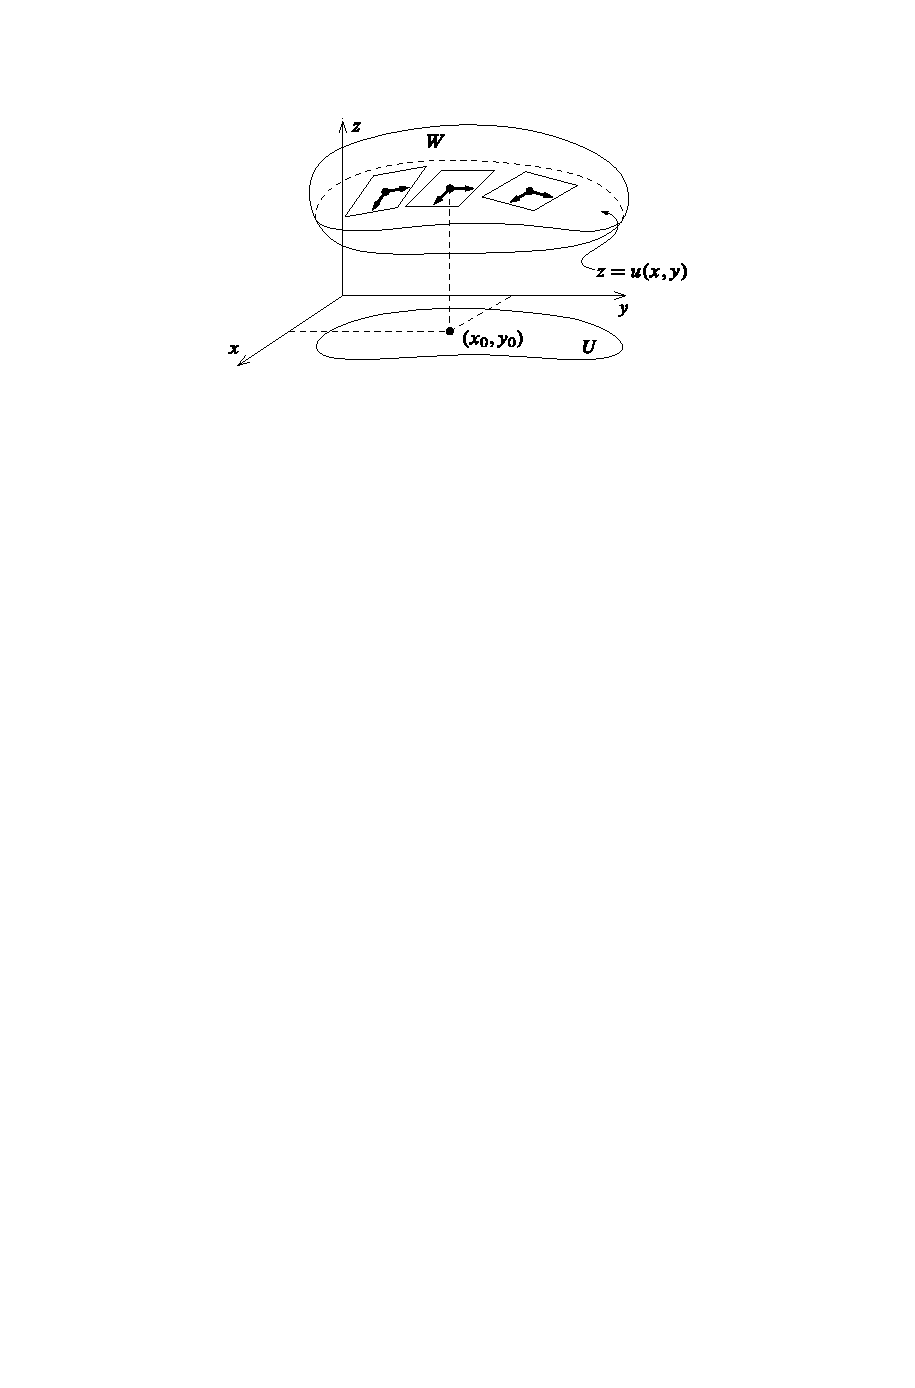
\includegraphics{pictures/overdetermined-PDE}
\caption{Solving for $u$ by finding its graph.}
\end{figure}

If there is a solution $u$ on an open subset $U\sub\R^2$, the map $F:U\to W$ given by
\[F(x,y)=(x,y,u(x,y))\]
is a smooth global parametrization of the graph $\Gamma(u)\sub U\times\R$. At any point $p=F(x,y)$, the tangent space $T_p\Gamma(u)$ is spanned by the vectors
\begin{align*}
dF\Big(\frac{\partial}{\partial x}\Big|_{(x,y)}\Big)=\frac{\partial}{\partial x}+\frac{\partial u}{\partial x}(x,y)\frac{\partial}{\partial z}\Big|_p,\\
dF\Big(\frac{\partial}{\partial y}\Big|_{(x,y)}\Big)=\frac{\partial}{\partial x}+\frac{\partial u}{\partial y}(x,y)\frac{\partial}{\partial z}\Big|_p.
\end{align*}
The system $(\ref{overdetermined nonlinear PDE two dim})$ is satisfied if and only if
\begin{equation}
\begin{aligned}\label{overdetermined nonlinear PDE two dim solution-1}
dF\Big(\frac{\partial}{\partial x}\Big|_{(x,y)}\Big)=\frac{\partial}{\partial x}+\alpha(x,y,u(x,y))\frac{\partial}{\partial z}\Big|_p,\\
dF\Big(\frac{\partial}{\partial y}\Big|_{(x,y)}\Big)=\frac{\partial}{\partial x}+\beta(x,y,u(x,y))\frac{\partial}{\partial z}\Big|_p.
\end{aligned}
\end{equation}
Let $X$ and $Y$ be the vector fields
\begin{equation}
\begin{aligned}\label{overdetermined nonlinear PDE two dim solution-2}
X=\frac{\partial}{\partial x}+\alpha(x,y,z)\frac{\partial}{\partial z},\\
Y=\frac{\partial}{\partial y}+\beta(x,y,z)\frac{\partial}{\partial z}.
\end{aligned}
\end{equation}

on $W$, and let $D$ be the distribution on $W$ spanned by $X$ and $Y$. Because $(\ref{overdetermined nonlinear PDE two dim solution-1})$ says that $T_p\Gamma(u)$ is spanned by $X_p$ and $Y_p$, a necessary condition for the system $(\ref{overdetermined nonlinear PDE two dim})$ to be satisfied is that $\Gamma(u)$ be an integral manifold of $D$. On the other hand, this condition is also sufficient: if $\Gamma(u)$ is an integral manifold, then $dF(\partial/\partial x)$ and $dF(\partial/\partial y)$ must both be linear combinations of $X$ and $Y$, and comparing $\partial/\partial x$ and $\partial/\partial y$ components shows that this can happen only if $(\ref{overdetermined nonlinear PDE two dim solution-1})$ holds.\par
A straightforward computation using $(\ref{overdetermined nonlinear PDE two dim compatibility})$ shows that $[X,Y]\equiv 0$, so given any point $p=(x_0,y_0,z_0)\in W$, there is an integral manifold $N$ of $D$ containing $p$. Let $\varPhi:V\to\R$ be a defining function for $N$ on some neighborhood $V$ of $p$; for example, we could take $\varPhi$ to be the third coordinate function in a flat chart. The tangent space to $N$ at each point $p\in N$ (namely $D_p$) is equal to the kernel of $d\varPhi_p$. Since $\partial/\partial z|_p\notin D_p$ at any point $p$, this implies that $\partial\varPhi/\partial z\neq 0$ at $p$, so by the implicit function theorem $N$ is the graph of a smooth function $z=u(x,y)$ in some neighborhood of $p$. It is easily verified that $u$ is a solution to the problem. Uniqueness follows immediately from Proposition~\ref{integral mani local struct}.
\end{proof}
There is a straightforward generalization of this result to higher dimensions. The general statement of the theorem is a bit complicated, but verifying the necessary conditions in specific examples usually just amounts to computing mixed partial derivatives and applying the chain rule.
\begin{proposition}
Suppose $W$ is an open subset of $\R^n\times\R^m$, and $\alpha=(\alpha^i_j):W\to\mathcal{M}_{m\times n}(\R)$ is a smooth matrix-valued function satisfying
\begin{align*}
\frac{\partial\alpha^i_j}{\partial x^k}+\alpha^l_k\frac{\partial\alpha^i_j}{\partial z^l}=\frac{\partial\alpha^i_k}{\partial x^j}+\alpha^l_j\frac{\partial\alpha^i_k}{\partial z^l}\quad\text{\textit{for all} }i,j,k,
\end{align*}
where we denote a point in $\R^n\times\R^m$ by $(x,z)=(x^1,\dots,x^n,z^1,\dots,z^m)$. For any $(x_0,z_0)\in W$, there is a neighborhood $U$ of $x_0$ in $\R^n$ and a unique smooth function $u:U\to\R^m$ such that $u(x_0)=z_0$ and the Jacobian of $u$ satisfies
\[\frac{\partial u^i}{\partial x^j}(x^1,\dots,x^n)=\alpha^i_j(x^1,\dots,x^n,u^1(x),\dots,u^m(x)).\]
\end{proposition}
